\part{Machine learning based detection of exoplanets using high contrast image spectra}
\chapter*{abstract}
Extracted spectra are an increasing part of exoplanet science, particularly with the advent of the James Webb Space telescope. 
The scientific goals of such spectra range from molecular characterization, molecular species detection to constraining abundances in exoplanet data.
In direct imaging the availability of spectra in high contrast images has allowed astronomers to detect exoplanets and characterize them.
With increasing data sizes and the availability of high resolution direct imaging spectra from high resolution spectrographs, there are both computational and accuracy limitations brought by the traditional techniques used to analyze these spectra.
The advent of advanced data science algorithms particularly machine learning algorithms have been suggested as an alternative to traditional spectral processing.
This part is dedicated to studying the effect of ML algorithms when used directly on spectra extracted from direct imaging data.
To that end we have two introductory chapters;
in the first one  we will first introduce data processing methods for direct imaging spectra and in the second we will then introduce ML algorithms and specifically the classes of algorithms used in this chapter.
This is followed by the data chapter in which we will define the science objectives and the data that is used to meet these science objectives.
This is followed by two methods chapters; 
the first of which describes the cross correlation based algorithm and the results it produces on the benchmarking scale and its scientific impact,
The second methods chapter describes the ML algorithms and their results
The final chapter in this part will discuss the results and derive a conclusion from both the experiments and finally define what next step this piece of research has motivated us to do.

\vfill
\startcontents[chapters]
\printmyminitoc{}
\chapter{Introduction to spectral data processing}\label{chap: III.1}
Spectral data was used in the previous Part by extracting the spectra from SADI data cubes.
We used the pixels as samples of spectra that are then cross-correlated with template spectra.
In order to make detections we had to define a SNR value by using the cross correlations values generated by cross correlating spectra extracted from different pixels.
In the previous part we explored spectra as extractions from individual pixels.
We cross correlated these spectra with template spectra and then reconstructed the maps with these replaced spectra.
We explored different spatial methods to make these spectra noise free and amenable to data processing.
The goal of the previous part was to understand whether spectral processing of spaxels can produce similar or different effects when taking into account the spectral features.

In this part, we will explore the detectability and characterization of exoplanets through spectra alone without considering the image dimension. 
The goal of this part is to study the detection and characterization of exoplanets whose spectra have been extracted from the spaxels.
In the absence of a spatial dimension, we lack the ability to produce SNR maps as in the previous part, we also miss the distinctive 2D Gaussian shape that indicates the PSF of the telescope on the exoplanet.
Therefore, the broad scientific goal of this part is to understand how much is detectability and characterization of exoplanets is affected by the absence of these key features.
This part will explore the efficacy of ML algorithms of detecting exoplanets and whether they can prove a viable alternative to cross correlation based detection techniques, and whether they can continue to leverage the simultaneous detection and characterization advantage that spectra lend to.

We will describe in this chapter the scientific contributions that spectra alone have produced to the field of exoplanet science, we will then describe briefly the different types of algorithms that have used spectra to make this science possible. 
We will then situate the importance of our research in this context of algorithms by describing the limitations of already present algorithms. 
We will then describe the various ML algorithms that are currently in use in Astronomy related to spectra.
We will then describe why we are motivated to use ML algorithms and which ones seem to be best suited for this job of identifying spectral features in the data.
\section{Exoplanetary spectral data from direct imaging data sets}
As described in the previous part, spectral data are produced using IFS enabled imaging instruments such as \citep[SINFONI, ][]{2004SINFONI} and \citep[GPI, ][]{2014MacintoshGPI}.
The disadvantage of having images with spectra is that it leads to a large number of spectra with just noise and just few spaxels with the exoplanet.
This sometimes leads to false positive detections in discovery campaigns.
In addition, exoplanets are very faint to be easily visible in images, particularly when the image is noisy.
However, it is also possible to not have an explicit spatial dimension, but still have extracted spectra through an IFS enabled instrument.
This allows us to have fewer but more targeted spectra with just one robust noise spectrum, the standard deviation of which can be used to estimate the noise in the observations.
For the purposes of this introductary chapter, we will  refer to such spectra as high contrast diffusion spectra (HDC).

Examples of such instruments include \citep[KPIC, ][]{2019KPIC} and \citep[HARMONI, ]{2022Jocou}.
KPIC is attached to the Keck telescope and is designed to have $\approx 50\%$ starlight suppression and is designed to detect faint exoplanets which are not visible in the image.
Typically, the best way to reduce stellar contamination is to image in wavelength where the stellar flux is low as compared to planetary emissions, the choice of wavelength thus falls typically in the near IR (between $1.4$ $\mu$m  and $1.9$ $\mu$m that corresponds to the H-band and between $2.0$ to $2.4$ $\mu$ m that corresponds to the K- band.
Therefore, these instruments operate in H and/or the K bands.
Typically, KPIC as an example, operates in a domain called high dipsersion coronagraphy which combines high contrast imaging and the medium to high resolution spectroscopy.
The high contrast portion imaging is achieved by feeding the light from the CCD in the telescope through single mode fibers placed at the exact pixel where the planet is present.
The light is then dispersed through medium to high resolution spectrographs with a fixed resolution ($R$) between $10,000-100,000$.
Typically, the $R$ is defined for the lowest wavelength $\lambda_{\rm{min}}$ as,
\begin{equation}
    R =\dfrac{\lambda_{\rm{min}}}{\Delta \lambda}
\end{equation}
where $\Delta \lambda=\lambda_2-\lambda_1$ for consecutive wavelength values $\lambda_2$ and $\lambda_1$.
Laboratory studies have shown, for \citep[e.g][]{2021Calvin}, that coupling the single mode fiber to the CCD pixel appropriately produces the best signal to noise ($\rm{SNR}$).
This $\rm{SNR}$, given the context of using just the spectra defines the `quality' of the spectrum that can be used for scientific processing.

Thus, we have direct imaging that observe a star system where a potential exoplanet is present, the light is gathered on a CCD chip which is then coupled with a single mode fiber to achieve a desired $\rm{SNR}$ and then dispersed through a spectrograph with a fixed $R$ to produce spectra of potential exoplanets.
This spectrum will then be processed similar to what we did in the previous part.
However, unlike in the previous part where we use real data, in this part we will simulate this behaviour without any biases on the efficiency of coupling or the fixed $R$.
In order to achieve this we will use synthetic data that is described in \Cref{chap:III.3}.




\section{Exoplanetary science from HDS}
Spectra from direct imaging instruments have been useful in different ways in the field of exoplanet science. 
Spectra from direct imaging are obtained, usually, through the means integral field spectrographs (IFS) and are typically mounted on larger telescopes that gather photons from the target e.g \citep[e.g][]{2004SINFONI,2019SPHERE} or single mode fiber based instruments such as \citep[e.g][]{2019KPIC}.
This results in gathering of photons in specific wavelength bands that are reflected off the surface of the exoplanet and therefore has the ability to probe interesting surface physics such as temperature, cloud profile etc, when they are appropriately retrieved \citep[e.g][]{2019PICASO}.

There are broadly two ways that these spectra can be used for a) detecting exoplanets based on specific molecules present in the spectrum or b) characterizing exoplanets by identifying the concentration of molecules present in the spectrum.
While detection is a fairly well defined term, meaning to be able to sensitively assert that an exoplanet is present based on spectral features alone, whereas characterization is a broader term that covers a broad swathe of definitions.
The simplest form of characterizing the exoplanet is to constrain the $\rm{T_{eff}}$ and $\log(g)$ of the exoplanet.
In this case the parameters are constrained with a clearly defined error bar for both.
This is usually the first step that follows any detection and spectra are the only data dimension that we have to perform this step.
Usually, we don't need even the spectral absorption lines to estimate $\rm{T_{eff}}$ and $\log(g)$ as shown by \citep[e.g][]{2023Cugno} for PDS70b, they are estimated using continuum modelling or using SED estimation as in the case the first time it was discovered by \cite{2019MesaPDS70}.
Typically, this is the go-to approach when constraining $\rm{T_{eff}}$ and $\log(g)$ is to use the continuum of the exoplanet and derive these with SED, but this only works for exoplanets that are far out from the stellar glare that will be easily characterized.
On the other hand for close in companions such as \citep[HD142527b, ][]{2018A&ChristiaensHD142527}, the continuum is fully dominated by the stellar glow and therefore the molecules present in the atmosphere alone are the indications to the $\rm{T_{eff}}$ and $\log(g)$.

Characterization can also be done in terms of molecular abundances \cite{2023Wangabund} on the surface of the planets, constraining metallicity and surface gravity of the exoplanets \cite{2023AlemanMetall}.
These type of characterizations are particularly interesting because they give us the following scientific details,
\begin{itemize}
    \item \textbf{Constraining the ages of exoplanet systems:} Molecular abundance ratios are crucial in determining how old an exoplanet and thereby its system is which allows us to lay constraints on its theory formation. The \textsc{C/O} ratio is one of the most common ratios that are inferred and \cite{2021Vandermarel} shows that this ratio can be used to constrain the transport rates of icy pebbles within the protoplanetary disks,
    \item \textbf{Constraining the composition of an exoplanet:} the composition of an exoplanet is one of the key attributes that makes exoplanetology truly alluring, according to \cite{2019Madhsudhan} this sort of characterization has resulted in the necessity for new instruments which has in turn lead to a state of `competitive exoplanetology'. Nevertheless, the abundance ratios, the depth at which these ratios are recovered are the only means that we know currently to infer the composition of an exoplanet. 
    \item \textbf{Constraining dynamic processes that define exoplanetary evolution:} molecular species opacities allow astronomers to lay constraints on the dynamic processes within the planetary atmosphere for \citep[e.g Brown dwarfs]{2020Phillips}
    \end{itemize}
In general,characterization using molecular abundances allow us to constrain both the age and rule out potential kinds of exoplanets \citep[e.g][]{2021Christiaens}.

For these kind of studies in addition to observed spectra from planetary systems, we require accurate theoretical models of what planetary spectra look like at different resolutions.
It is prudent to model these spectra in the infra red starting for $0.9$ $\mu$m up to $7$ $\mu$m where the ratio of planetary flux to stellar flux is higher. 
A number of detailed spectral models exist starting with high resolution molecular models produced in lab settings such as ExoMol \cite{2012Tennyson}, detailed atmospheric models that are amenable to spectral retrieval such as PetitRadTrans \cite{2022Molliere}, specialized cloud and atmosphere models that are suited to studying exoplanetary atmospheres such as PICASO3 \cite{2023Mukherjee} and generalized absorption spectra that are more suited to constraining specific properties of the exoplanet such as $\rm{T_{eff}}$ and $\log(\rm{g})$, which is what we use in this project named BT-SETTL \cite{1997Allard}.

While retrieval is notoriously difficult in practice, it is possible to use theoretical spectra and model specific molecules on the surface of the potential exoplanet and thereby characterize them based on mass and temperature.
In order to narrow the scientific scope and to limit the complication of scientific inferences, this thesis will primarily limit itself to characterizing the $\rm{T_{eff}}$ and $\log(g)$.
This also allows this thesis, to explore the effectiveness of the characterization of exoplanets by using the accuracy of characterization of $\rm{T_{eff}}$ and $\log(g)$ as it uses the same features.
These features are also the same molecular absorption lines that will allow us for instance to constrain specific molecular abundances.
Hence, we use these two parameters as proxies to define the ability of an algorithm to characterize exoplanets.
%Such algorithms rely on the accurate modelling of the exoplanet spectra provided by accurate and detailed modelling of the physics necessary to 
%Spectra thus obtained comprise of photons emitted by the star but also the photons reflected off the exoplanet.
\section{Algorithms that detect and/or characterize exoplanets using high contrast diffusion spectra }
%Spectra are particularly useful tools in the infrared where most of the planets are bright as compared to their host stars.
This thesis will constantly refer to algorithms in two broad categories based on how they produce results from the spectra.
These algorithms all either use non-ML based techniques such as cross correlations, forward modelling etc or they use ML based techniques that infer results using ML algorithms that have either been trained with such data or are somehow very specific to using spectra.

Algorithms that use spectra typically work on specific characterizations of a detected exoplanet. 
Atmospheric characterizations are performed by either retrieval algorithms \citep[e.g][]{2017Lavie} or by forward modelling \citep[e.g][]{2023PalmaBifani} the extracted spectra to derive specific atmospheric properties such as carbon to oxygen $\rm{C}$/$\rm{O}$ ratios in the atmosphere of the exoplanet.
Broader characterizations of the exoplanet could be limited to constraining the $\rm{T_{eff}}$ and $\rm{\log(g)}$ with errorbars using log-likelihood ratios obtained through forward modelling \citep[e.g][]{ruffio2019radial} particularly in cases where spectral lines themselves are not well resolved.
In this section, we will discuss algorithms that have one processing criteria in common, they take as input raw spectra from instruments such as KPIC and produce scientifically interpretable and publishable results.
In their turn, these algorithms have been benchmarked for their performance.
In this section we will present a brief summary of the type of algorithms and their science results.

\subsection{Non-ML based spectral inference algorithms }
Post processing for detection and/or characterization of high contrast spectra is different from other spectral post-processing (for example other data acquisition methods such as transit photometry) because of the pecularities unique to high contrast imaging.
The first step, though this thesis does not focus on this step, would be to calibrate the extracted spectra from an instrument.
This calibration step usually involves solving for the wavelength solution so that the resulting vector from the instrument is mapped to its equivalent wavelength values such that each photon value in the vector corresponds to a wavelength vector.
Once this is done, a major problem is the continuous presence of stellar contamination in terms of the stellar continuum in most spectra, particularly those spectra of exoplanets that are at smaller separations from the host star.
Thus, processing of spectra requires the equivalent of the PSF subtraction performed for ADI images.
This has to be followed, by some way of comparing known exoplanet models to the spectrum of the candidate exoplanet in such a way that any residual stellar contamination does not significantly impact this comparison.
Finally, the results of this comparison have to be interpreted so that it has scientific relevance.

\paragraph{Stellar contamination subtraction methods:\\}
The most used stellar contamination subtraction methods is spectral differential imaging \citep[SDI, ][]{2002SparksSDI} which accurately measures the stellar spectrum and subtracts from the data leading to relatively stellar contamination free spectra.
SDI creates several high frequency artefacts which are somewhat resolve with the use of high resolution spectral differential imaging \citep[HRSDI, ][]{2019Haffert} and modified HRSDI \citep[mHRSDI, ][]{2020Xie}.
For spectra in HDS domain, we have continued the same sort reference spectra creation and the adoption of removal of low frequency artifacts.
Usually, this leaves behind mis-subtracted residuals, these are known as speckles in the spatial domain, but there is known equivalent or study in the spectral domain. 
In the spatial domain the speckles are typically tackled using \citep[PCA based algorithms, ][]{2020Xie,2018Hunziker} where after performing procedures such as SDI, further principal components are computed from the image dimension and then subtracted to remove the unsubtracted residuals. 
There has also been a few attempts to combine the advantages of having both image and spectral data by combining angular differential imaging (ADI) and spectral differential imaging techniques in an optimal manner \cite{2021Kiefer}.
This is akin to the analysis we have performed in Part II.
Principal component analysis, typically applied to the image domain \cite{2012Amara}, have been adapted a combination of both spatial and spectral PCA.
%Even then, other than molecular maps, the algorithms do not leverage the information inherently available in spectra to detect exoplanets.
Thus, while we are able to perform basic subtractions there is no comprehensive subtraction of stellar contamination.


\paragraph{modelling the residual spectral features:\\}
Once the stellar contamination subtraction step is completed, algorithms typically now transform the data making it amenable to interpretation and statistical analysis.
There are two broad ways that spectra are processed to characterize them, one would be the so called forward modelling where an analytic function is fit to the data along with a model of noise and the best fit is chosen as the exoplanet model.
An example of such modelling is \citep[BREADS, ][]{2023Agrawal} which uses the standard forward modelling principles set out in \cite{ruffio2019radial} which has been since then in the detection of water and carbon monoxide in HR8799 \citep[][]{2021Ruffio}.
Detailed modeling of the spectral shapes has allowed us to identify orbital parameters as well \cite{2022BWang} where accurate retrieval techniques can be used to constrain the carbon to oxygen ratios as well.
In the realm of medium resolution spectroscopy, it is still possible to limit the science question to if specific molecules such as $\rm{H_2O}$ and $\rm{CO}$ are still detectable and this is performed with radial velocity searches through template cross-correlations \citep[e.g][]{2021Ruffio}.

The other type of processing is using cross correlations of templates and the spectra itself as we did in Part I. 
This type of processing has been particularly popular when detecting specific molecules using \citep[for e.g Molecule maps][]{2018AHoeijmakersMM}. 
Cross correlations have an advantage because of their simplicity and ease of interpretations. 
On the other hand the cross correlation coefficients themselves are noisy and the most consistent interpretations need several noise realizations.
These do not easily lend to HDS data, in this thesis we use the formalism established by \cite{ruffio2019radial} to define cross correlation noise.

\paragraph{interpreting the results:\\}
Both forward modelling and cross correlations result in produces either mock spectral models or cross correlation coefficients that are subject to interpretation.
This interpretation is typically made in the context of statistical $\rm{SNR}$ which is computed as a ratio of the signal cross correlation coefficients and standard deviation of the noise correlations. 
For the forward models the model spectrum is cross correlated with model spectrum produced by the forward model whereas it is also possible for instance to directly cross correlate the spectrum with a template directly.

The $\rm{SNR}$ is then computed for several molecules and thus it is possible to predict if a particular molecule is present if the signal is $5\sigma$ over the noise i.e $\rm{SNR}\ge5$.
Once the presence of an exoplanet molecules are detected, characterization consists of a few more steps in order to derive properties such as abundance ratios, orbital parameters etc.
Typically calculating abundance ratios involves `retrieving' the spectra from a set of atmospheric models as in \citep[for e.g deriving the C/H ratios][]{2022Xuan}.



%It is also possible to turn this question of whether certain molecules exist in the spectra to \textit{where} these molecules exist relative to the host, particularly with direct imaging.
%This kind of analysis is provided by molecular mapping techniques \cite{2018AHoeijmakersMM} where a spatial map is constructed from the cross-correlations of template spectra for each spaxel.
%This has proven particularly useful when trying to detect exoplanets where the planet preferentially radiates in specific wavelengths and is dim in the rest \citep[e.g][]{2019MesaPDS70,2019Haffert}.
%This is usually dependent on the SNR of the extracted spectra themselves.
%Techniques such as molecule mapping \cite{2018AHoeijmakersMM} have been particularly useful to detect exoplanets in specific bands.
%In addition to providing us with such molecule detection maps, spectra also allow us to characterize exoplanetary systems \cite{2018A&ChristiaensHD142527,2019MesaPDS70,2019Haffert} with their constituent molecular species. 
%This is also useful to make a precise atmospheric characterization of exoplanets already detected through other methods \cite{2022Ruffio}.
\subsection{Use of machine learning (ML) algorithms in analyzing astrophysical data and spectra}
Machine learning in the current age of big data has produced algorithms that are capable of analyzing large amounts of data with remarkably small processing times.
They have also proven to be particularly using unsupervised clustering and data mining \citep[e.g][]{2019Baron,2010IBall,2014IVESCI}.
They application of ML algorithms have been particularly of note in classifying stellar spectra \citep[e.g][]{2018Miettinen,2018Naul}.
The analysis of stellar spectra using AstroNN has shown promise even for high resolution spectra \cite{2019Leung}.
Application of artificial neural networks and particularly deep neural networks to exoplanet detection is now regarded as an established method in astrophysics \cite{2020Fluke}.
The exoplanet community has benefited from the use of deep neural networks for Kepler light curves \cite{2018Pearson}, for direct imaging detection \cite{2018Gomez} and to model the PSF model of an instrument \cite{2022Gebhard}.
ML algorithms such as PCA have shown that they can be quite well trusted to model the noise in data \cite{2016A&AGomez} and to model the PSF of the instrument which results in high fidelity subtraction of the stellar components \cite{2014Meshkat}.
In addition, deep learning algorithms such as SODINN \cite{2018Gomez} have demonstrated the ability to detect high contrast companions with fewer false positives.
This has motivated their use in new missions and surveys such as the Large interferometer for exoplanets (LIFE) \cite{2021LIFE}.
In this context, ML algorithms were considered to be of value to the research question that this chapter addresses.
The ML algorithms attempted in direct imaging addresss either the question of PSF subtraction \citep[e.g][]{2022Gebhard} or try to use the spatial noise variance to discriminate between pixels that contain noise and those that contain the exoplanet \citep[e.g]{2018Gomez}.
These methods do not take into account the spectral absorption lines that uniquely identify exoplanetary absorption, which in turn can be considered exoplanetary signatures. 
Some attempts with using spectral features were not particularly successful \citep[e.g][]{2020Fisher} at learning these spectral features unlike \cite{2017RAALi} does for stellar spectra.
However, at this point there still remains the question of why it is necessary to explore the use of ML with spectral data.

\section{Limitations of current methods}
Molecule maps \citep{2018AHoeijmakersMM} are considered suitable for detecting species of molecules of warm Jupiters or cool M-dwarfs \cite{2023Malin} and has been used to further characterize the existence of certain molecules in well known companions \citep[e.g][]{2018Petit}.
One of the greatest limitations with applying techniques such as molecule maps is that they are applied when the existence of an exoplanet is well known and though they lend to astrometric characterization of molecules, it does not allow a truly `blind' search to commence.
In other words, while molecule maps detect the presence of molecules they do not detect the companions themselves, or at any rate they are not designed for a blind search for companions.
In the previous part we redetected HD142527b and produced SNR maps by taking into account all the molecules present in the spectrum.
In the previous part we also demonstrated that it is possible to produce SNR maps of such extracted spaxels and thereby detect a companion and that such a detected companion can also be characterized through the means of characterization matrix that we demonstrated for HD142527b.
Molecule maps and the cross-correlation maps constructed in the previous chapter, rely on some knowledge of spatial noise diversity and the spectral resolution of the spectra play a limited role in detection of the exoplanets.
High resolution spectra can be quite advantageous particularly with forward modeling the spectra \citep[e.g]{2021Ruffio,2021Wang} where spatial data is not available.
However, forward modelling is still a method to \textit{choose} a template that would be cross correlated with the sample exoplanet spectrum.
This brings into focus the importance of the cross correlation as the main engine of comparing spectra and identifying when a template matches the target spectrum.
While there are several algorithms that perform cross correlations and template matching, a unified framework that allows an astronomer to detect and characterize the exoplanet based on the spectrum is still missing.
Existing algorithms are also fine tuned to work with non-ML inference algorithms but a comprehensive study into how amenable these processing steps are with ML algorithms is missing.

Data sizes and the number of spectra available are also on the increase with the advent of James Webb, therefore there needs to be a scalable, accurate and somewhat model independent way to use these high resolution spectra to detect exoplanets in direct imaging.
Computational speeds also are problematic when a large number of forward models need to be run to rule out various hypotheses.
Therefore, the need of the hour is to be able to design an algorithm, which learns specific features which discriminate correctly between the spectra of an exoplanet and those of a star and those of noise.
We also need an algorithm that will be perform similarly for both high and low contrast exoplanets and whose computational complexity does not scale out of bounds for higher resolution spectra.
In this context, ML algorithms are appropriate to be tested with the current suite of inference algorithms already present in the literature.
The question however still remains in terms of why we expect ML algorithms to be effective for this problem.
%We can, therefore, now use spectra with versatility in order to detect and characterize a companion. 
%We also see that ML algorithms are able to detect the presnece of a companion with some degree of astrometric precision.
\section{Motivation to use ML algorithms for identifying spectral features of exoplanets}
%In the previous chapter we have seen that we can use cross-correlation to produce correlation maps which can then be used to produce detection maps.
In the previous part we discovered that detection of exoplanets using spectral data can be done through cross correlation primarily because of the presence of absorption lines in H and K bands.
This was particularly visible when we cross correlated with parts of the spectrum and saw the differential $\rm{SNR}$.
This clearly indicates that data features are not uniform, but are present in different wavelength ranges in the spectrum, this is also the feature set which is utilized for \citep[for e.g ][]{2019Leung} to classify stellar spectra.

However, how effective is an ML algorithm when compared to a standardized cross-correlation algorithm that is described in the previous chapte?
However, is there any relative benefit of using ML algorithms in place of a standard cross correlation and SNR map based detection regime?
Consequently, does this have characterization benefits that is naturally produced by the cross correlations?
What are the ML algorithms that are best suited to this form of analysis and would these `best in class' algorithms provide any advantage to exoplanet detection?
The motivation of this experiment is thus two fold, to begin with we need to define the variables about which we will quantify the effectiveness of an ML algorithm.
The second objective is to verify whether the performance of a well trained ML algorithm offers an advantage to cross-correlation for the same data.

Thus we have organized this part to describe the data that is used to make the comparison, the algorithms used and then finally our conclusion.
This chapter will describe the methods we use to produce data that can be used to test these questions.
We will then describe the control of thse data with the use of parameter `knobs' that allow us to calibrate the effectiveness of the algorithms that we are comparing against.
We will then describe the algorithms that were used during these experiments to compare against the cross correlation of template spectra. 
We will then describe the metrics used to compute the `effectiveness' of an algorithm.
This will the be followed up with describing the results produced by cross correlation and producing thereby the benchmark that is set for the ML algorithms to achieve in order to be called at least `as effective' as ML algorithms.
We will describe these benchmarks for both detection and characterization.
We will then describe results obtained by  cross correlation when the `knobs' are at different levels, for both detection and characterization.
We will then describe the preliminary results for the ML algorithms that will inform us why ML:algorithms cannot be compared with cross correlations.
We will then discuss the reasons for why ML algorithms are not suitable to replace cross correlations in this fashion.
Finally, we will conclude this chapter with a discussion on how we could potentially leverage the power of ML algorithms to improve detectability limits, and leverage what we have learnt from this chapter.

\chapter{Introduction to machine learning algorithms}
\label{chap:III.2}
Machine learning (ML) algorithms are considered a class of algorithms that learn intrinsic relationships in the data in order to predict specified outputs that depend on these intrinsic relationships in the data.
These relationships between specified outputs and the data can be learned in one of three well known ways,
\begin{enumerate}
    \item \textbf{Unsupervised learning:} where the ML algorithm exploits the intrinsic relationships within data to learn features and use such features to derive the desired output without any external interventions.
    Algorithms in this class are typically used with data where intrinsic relationships in the data are not well established a priory.
    %might be very useful to derive the desired output.
    For example, unsupervised K nearest neighbors algorithms are frequently used to identify clusters within the data that might indicate data grouping which is not easily understood such as looking for data that could be analyzed for transients \citep[e.g][]{2022AleoTransients}, or finding cluster groups in open cluster data \citep[e.g][]{2022cluster}.
    Within Astronomy principal component analysis is a very well known unsupervised ML algorithm typically used in identifying structures in the data that can be discarded.
    Unsupervised ML algorithms are particularly useful for instance in anomaly detection \cite{2023EJASPanomaly}.
    Selecting parameters in the data which will enable other ML algorithms to perform better on the data can also be achieved through unsupervised methods \cite{2023PatRe.14209676H}.
    Principal component analysis is particularly useful in detecting such useful parameters in the data and has been proposed for instance to detect oceans in exoplanet data \citep[e.g][]{2022RyanOCeans}.
    Within the field of high contrast imaging unsupervised ML algorithms have been used in the package \citep[PACO,][]{2023Chomez} and \citep[VIP, ][]{2023Christiaens} also provides this capability. 
    \item \textbf{Supervised learning:} where the algorithm is shown multiple combinations of relationships between desired outputs for a set of inputs over multiple times and thus `trained' to learn the relationship between the input and the output.
    Algorithms in this class are typically used when there is a large amount of labelled data and typically when the relationship between the desired output and input is well known.
    This class of algorithms are also very effective when the desired output represents a non-linear combination of inputs for instance inferring for instance that a picture contains a cat from the presence of whiskers, eyes, nose etc in the picture.
    A famous example of such supervised learning was the handwritten digit recognition where a ML algorithm is trained to recognize handwritten digits in the US postal system and has now been improved on with the latest advances in supervised learning \cite{kussul2004improved}.
    This class comprises of a large set of algorithms spanning from \citep[neural networks,][]{gurney1997introduction} to \citep[random forests,][]{breiman2001random} to modern day \citep[transformers,][]{vaswani2017attention}.
    The advantage of supervised algorithms is that they are able to learn many complex relationships in the data. 
    However, the intrinsic problems of this class is that it requires a large amount of data, where this is relationship is well known.
    Supervised learning schemes suffer from the significant problem of learning the unintended relationships in the data when it is not trained appropriately or it is tested with wrong data.
    In the same example as before, if the algorithm is trained to recognize only cats and we present a dog, it will indeed mis-identify a dog as a cat because of the similarity of the features.
    It is also possible that while learning the possible relationships between the images and the presence of a cat, the algorithm learns that the any indoor setting is a picture of a cat because of our data contained only indoor cats.
    \end{enumerate}
In this thesis, we focused only on supervised learning for the following reasons,
\begin{itemize}
    \item the goal of the my thesis is to derive the presence of an exoplanet given certain discriminatory conditions in my input such as the spectral features corresponding to the planet.
    Such `conditions' are typically called features in ML algorithm training.
    \item a good prior knowledge of such a relationship exists (and is proven using non-ML algorithms such as cross correlation) and a large number of similar datasets exist for me to train a supervised algorithm,
    \item and finally, supervised algorithms allow us to specify the kind of output we need in astrophysics rather than relying on pre-existing relationships within data.
\end{itemize}
The act of producing data pairs of input and desired output is known as `labelling' and is typically carried out before training or testing any algorithms.
The desired outputs which are the result of a specific input combination are respectively called the `label' and the `data'. 
The data, thus, consists of multiple intrinsic parameters which as stated before are called features and the ML algorithm will typically learn which of these features are important for the desired output.
In our case the desired output is whether an extracted spectrum is that of a planet and the features that we use to arrive at this result is the spectral absorption bands.

\section{Types of supervised algorithms}
\label{sec:classifcation and regression}
Supervised learning can be further categorized based on the type of desired output as a regression and classification problems.

\textbf{Regression:} 
When the output of the supervised learning algorithm is a floating point number such as the distance or the intensity then such problems are called regression problems. 
Regression problems are usually adopted when the ML algorithm is meant to produce an unbounded output (except by the intrinsic rules set by the case itself for instance distance cannot be negative). 
This is also useful when we don't know precisely what the expected output is for a specific input, for instance distance between two points in an image can have a infinite values and this changes from each input to another.
Within regression problems, we also have types of regression based on the bounds of the output parameter.
For instance if the bounds are between $0$ and $1$, such regression is known as logistic regression.
The fundamental limitation of the regression problem is that there is an intrinsic uncertainty in the result. 
If sufficient information is presented then this uncertainty can be constrained to be within a few percent.
However, in some cases the output itself is constrained to be within a few finite values. 
Such class of problems are called classification problems.
Astronomy has many regression problems where for example galaxy photometric parameters have been estimated using machine learning algorithms \cite{2022YinAEparameter}.
Time series forecasting in astronomy has also been framed as regression problem \cite{2018Modred}.

\textbf{Classification:}
Classification problems are where the output classes are already well known, for example when the input is a set of words the machine learning algorithms classifies these words in to the emotions they are associated with such as happiness, anger etc. 
Classifiers have been also used to predict for instance liver lesions \cite{2023Nanda} in medical imaging. 
In astronomy classifiers have been used to differentiate between stars, blazars and quasars \cite{2023Zhao} in WISE data.
They have also been famously used to morphologically classify galaxies in the SDSS DR17 \cite{2019MNRASFischer}.
Classifiers in exoplanet direct imaging have been used by \citep[SODINN, ][]{2018Gomez} and \citep[NA-SODINN][]{2023Carlito}.
While classification has the adavantage of knowing the precise set of values that needs to be predicted, it also has the problem of the classes themselves being categorical.
For instance, \citep[SODINN, ][]{2018Gomez} wants the class of $C^{+}$, which is not a numerical value.
Typical classifiers work with either neural networks or ensemble classifiers such as \citep[Random Forests, ][]{breiman2001random} that produce floating point outputs.
In order to convert these numerical values we do the following two step process,
\begin{enumerate}
    \item For an $n$ class classification We first create an $n-1$ sized array.
    Therefore, a $10$ class classifier will output an $9$ element array, 
    \item we then encode the classes using routines such as \citep[One hot encoding][]{harris2010digital} that allows to convert a categorical class into a encoded value, where each position in the array is encoded as a $1$ for its corresponding class.
    The case where all array elements are $0$ also corresponds to a class, thereby covering all classes
\end{enumerate}
This encoded data is now considered as the value that the ML algorithm needs to predict.
Thus the ML algorithm will predict a value for each position in this array, typically values will range between $0$ and $1$ for each position following the sigmoid function.
Each value is thus a probability of the class and thus the class that the algorithm predicts would be the position with the highest probability.
We also at time provide a threshold above which the highest probability is accepted and this becomes the decision boundary of the classifier.

While classifiers are some of the most widely used type of supervised algorithms, they also suffer from the issue where some classes are better represented than the others. 
They also require large number of labelled examples.
These examples have to provide adequate representation of each of the classes, the noise distribution of the noise in each of these class samples should also mimic realistic noise in the data and finally, the samples themselves have to be representative of the data that the algorithm is expected to realistically classify.
In order to meet these requirements, we adopt training methodologies to adequately `train' an algorithm and then adopt specific testing methodologies to realistically estimate the performance of such algorithms. 
These are common for all supervised algorithms, sometimes the testing methodology can still be adopted for unsupervised algorithms as well.
In this thesis when we say ML algorithms it is taken to mean supervised ML algorithms.
\section{Training and testing supervised algorithms}
When generating labels for supervised data there is an intrinsic relationship between the data and its corresponding label.
This relationship could be either linear or non-linear and can thus be mapped to generate the output $y$ from input data $x$ as,
\begin{equation}
    y = f(x)
    \label{eq:y=fx}
\end{equation}
where $f(x)$ represents a function mapping $x$ to $y$
A special case of this linear relationship would be a straight line where $y$ and $x$ are related by its slope $m$ and interecept $c$,
\begin{equation}
    y =  m x + c
    \label{eq:line}
\end{equation}
ML algorithms have been trained in various contexts to derive such relationships between $x$ and $y$ based on large amount of data.
Such a process by which the ML algorithm is tuned to mimic $f(.)$ is called `training'.

Training requires sufficient number of data points that correspond to the expected output $y$. 
The function $f(.)$ is represented by the parameters of the ML algorithm which allow it to produce $y$  given $x$. 
These parameters differ based on the ML algorithm in question, their tuning will be explained in detail in the section corresponding to those class of algorithms.
In order to train an algorithms, we must first prepare the data so that this training is adequate, but not so targeted that the trained `model' can no longer generalize to new data.
The data usually has two characteristic elements, the data or $x$ which consists of images or spectra and the desired result or target output $y$ which is in our case whether the input corresponds to that of a warm Jupiter or not.
In this case it is important that ML algorithm learns the generalized features in the data corresponding to the presence of a warm Jupiter but avoids learning noise structures present only along with the warm Jupiter which would be a systematic of data acquisition.
Typically, this is solved with acquiring data with enough different types of systematics which would convince our model to learn only the common features, since this is not possible to achieve in practise we try to generate large amounts of data and try to evaluate how generalized the model is.
In order to ensure this we first split the data into three parts
\begin{enumerate}
    \item \textbf{Training part}: Usually this comprises of $80\%$ of the data present and is the main engine to train the ML algorithms.
    The training is usually carried out by passing the $x$ through the ML algorithm and `comparing' the output of the algorithm to the true label.
    Usually this comparison is carried out using loss functions such as \citep[cross entropy loss, ][]{1990ZhangCNN}.
    This loss is then minimized over multiple examples by tuning the algorithm until the same error on a part of the dataset not used for training reaches a low minimum value
    \item \textbf{Validation part}: This is the part of the dataset where the loss is tracked until it reaches a low minimum value to signify the end of training. 
    This comprises of $\approx 10\%$ of the total data and is removed from the data before commencing training. 
    The difference between the output produced by passing the validation data through the algorithm and the true labels is not used to tune the ML algorithms but rather serves to mark the state of the algorithm.
    When this difference reaches a minimum low value the training is stopped and the generalization of the algorithm is tested.
    \item \textbf{Testing part:} This part corresponds to $\approx 10\%$ of the total data.
    This part of the data is never passed through the ML algorithm until the error for the validation dataset reaches a low minumum value.
    The test data is treated as the final test data which can be used to benchmark how much the model has generalized. 
    This is also serves to inform if the model has not learnt the features and has just learnt specific noise structures present only in the training data but not present in the test data.
    Note that this does not rule out systematic noise that is present in the entire dataset, and in fact unless the dataset is a very good representation of real variance in data, the results on the test set is usually a clue to the performance of the training.
\end{enumerate}
Thus, the training, validation and test parts make up $100\%$ of the data. 
Typically, when data sizes are small the validation and test are reduced to $5\%$ each.
Once the test part of the data has been passed through the algorithm, the `model' is now deemed as `trained'. 
The quality of the training reflects in the test scores. 
When the test scores are low but the same scores when computed for the training are high, it indicates that the model has not generalized very well.
This is also known as `overfitting'. 
This term refers to the idea that model not only trains on the data features but also on the random noise in the data.
Such a model has to be retrained once again with appropriate mitigation strategies such as regularization in order to avoid such overfitting.
\textbf{Regularization:} is defined as small penalty applied to the error so that the error does not easily minimize for small changes in the data, presumably produced when the model fits the noise.
The converse issue is also possible where the testing error and the training error both are similar but high. 
This is a case of `underfitting' where the data characteristics or features are not sufficiently high to produce a well trained model that generalizes.
In such cases, we have numerous strategies to increase the exposure during training of the algorithm to data features.
\begin{itemize}
    \item \textbf{Feature engineering:} is the strategy where we identify aspects of the data which lead to better validation accuracy and lower training error. 
    We then train the ML algorithm with more of those data samples where such features are present or alternatively train the algorithms with only those features present where we have low validation error.
    \item \textbf{hyperparameter tuning:} in this strategy we change the parameters of the ML algorithm so that it produces lower training error and higher validation accuracy.
    The hyperparameters are subject to which ML algorithm we are training, sometimes tuning such hyperparameters can be difficult to achieve by hand and therefore we undertake a hyperparameter search where we systematically vary the values of the hyperparameters until we achieve the desired accuracy and error combination.
    \item \textbf{data augmentation:} is a method by which we apply specific transforms to the data that systematically provide increased diversity in the features and provide additional noise so that the intrinsic noise is not memorized.
    Thus it also acts as a regularizer.
\end{itemize}

In the subsequent subsection we describe the two broad types of algorithms used in this chapter namely ensemble algorithms of which we will explain the random forests and multi layer perceptrons of which we will describe deep neural networks (DNNs) and autoencoders (AE).
\section{Random forests} 
%Basic idea of ensemble classifiers
Ensemble methods rely on the fundamental idea that an ensemble of methods when polled together produce a reliable and predictive result.
These type of learning methods known as ensemble methods or algorithms was initially proposed with the use of \citep[decision trees, ][]{breiman1998arcing}.
This bit of research was followed by the seminal work where it was shown that \citep[Random forests, ][]{breiman2001random}, which are a collection of decision trees indeed produce smaller test errors than the original decision trees algorithm.
Since then Random forests have been the most sought after algorithm to perform machine learning tasks.
In the field of exoplanets we have instances of the successful use of random forests with \citep[SOFIRF, ][]{2018Gomez} and with \citep[RF, ][]{2020Fisher}.

In this thesis we use the random forest algorithm developed with \citep[scikit-learn, ][]{2011JRFsklearn}.
The basic unit of a random forest is a decision tree.
As the name suggests a decision tree is step by step evaluation of many decisions, which are made based on the data.
Decision trees are frequently used even outside of the ML algorithms to evalaute everyday chocies such as where to eat etc.
A decision tree consists of the following parts:
\begin{itemize}
    \item \textbf{root:} which is the start of the decision tree and is typically the first decision that needs to be made for instance, "Do we want to eat out today?"
    \item\textbf{nodes/leaves:} which is typically a new decision that needs to be made but is only influenced by the previous decision step i.e a node is created when we decide that we do want to eat, however a new decision has to be made about "what food do we want to eat"
    \item \textbf{termination leaf/node:} which is the final decision that is reached and is typically the end of the tree.
\end{itemize}
Depending on how many questions need to be asked and what is the kind of decision that is needed, these trees can be very deep and have many leaves.
A sample tree is show in Fig~\ref{fig:dt}.
This is a typical tree used to evaluate the species of an Iris flower.
This decision tree was expressly chosen indeed for its explanatory value where different characteristics of the Iris flower are used to make choice which finally determine the class such as petal length and width.
\begin{figure}
    \centering
    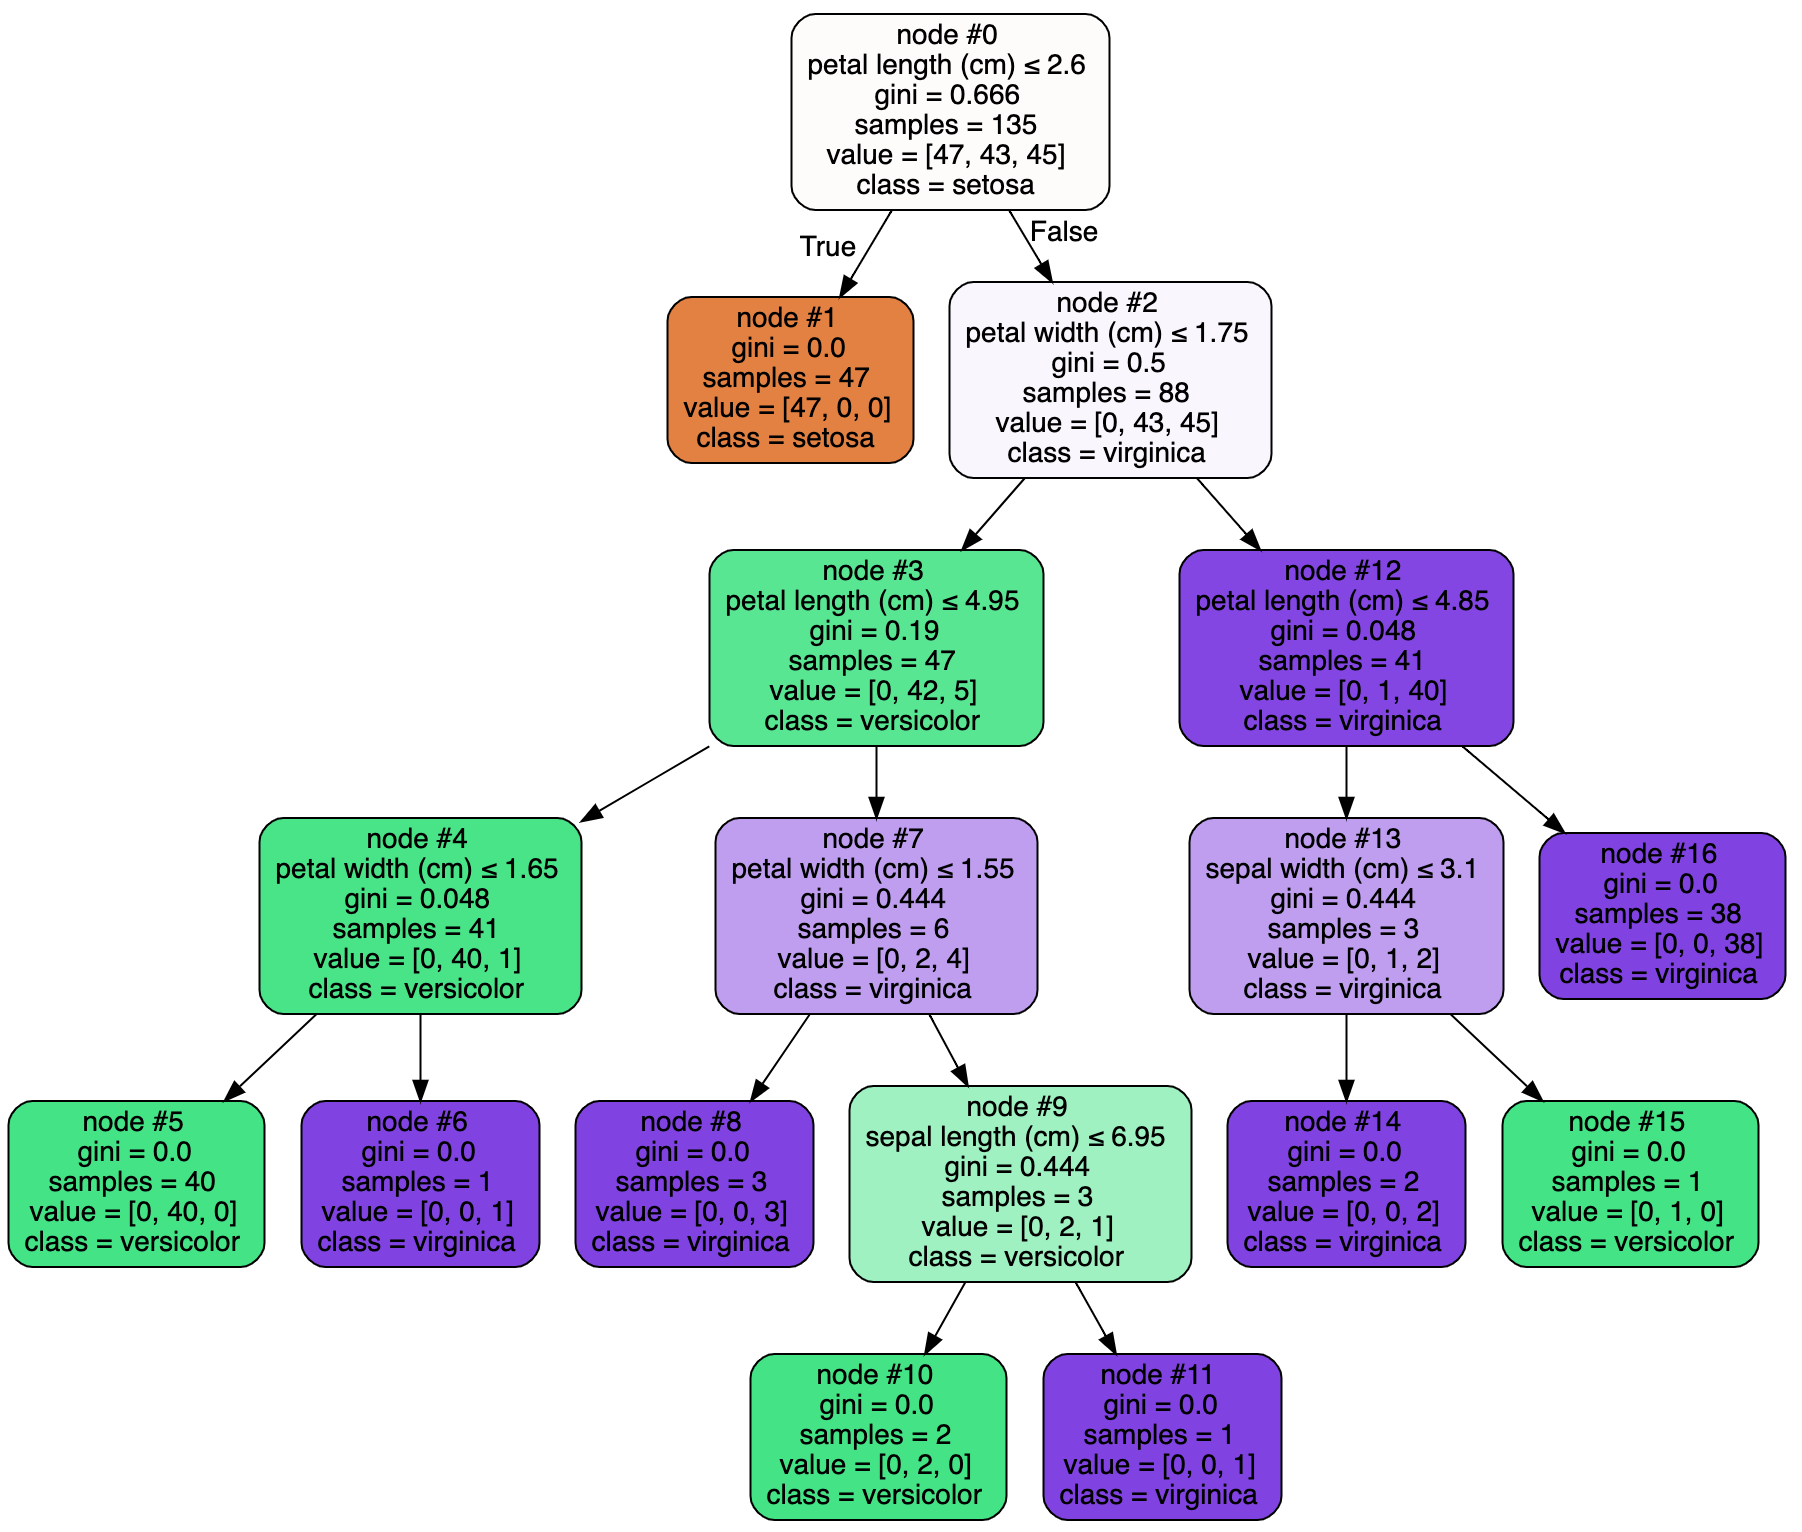
\includegraphics[scale =0.5]{images/Chapter3/decision_tree_model-2609977862.png}
    \caption{A sample decision tree}
    \label{fig:dt}
\end{figure}
An ensemble of many such decision trees result in a `forest' of decision trees which are collectively a `random' forest.

Random forests typically have a number of useful tunable parameters, these parameters are used to both regularize overfitting and improve underfitting.
The most common hyper-parameters that are tuned for random forests are the \texttt{n\_estimators} which are the total number of decision trees in the forest.
A key feature of the random forest is its feature explanability, typically the use of its feature importances, which explain the importance of the different data features in predicting the output of the random forest.
In the example of the Iris species classification, Fig~\ref{fig:RF sample FI} shows the feature importances in predicting the same species as in Fig±\ref{fig:dt}.
The feature importances are relative measures such that the sum of the feature importances is always $1$.
As with the decision tree, the random forest uses multiple features to regress/classify the data and arrive at the desired output.
As it does this process it uses different features, for example in the case of the Iris flower species classification, it uses the petal width as the most important parameter to make this prediction.
This is quite insightful in two ways,
\begin{enumerate}
    \item it is possible to intuit some understanding on the working of the random forest itself by knowing that some features are more relevant to make the desired predictions.
    This is usually the case when we know that the output depends on a few parameters but we are not sure which parameters act as features for the random forest.
    \item it is possible that we have several parameters (as will be the case in my thesis) that could be used to produce the desired output however, we are not sure if this is necessarily true. 
    For example, we have several spectral bins where the absorption lines corresponding to these of an exoplanet are present but we don't know which of these absorption lines allow us to detect and characterize an exoplanet.
\end{enumerate}

Thus, feature importances form the basis to evaluate the features of the data that were learned by the random forest.
This becomes relevant in multiple scenarios, 
\begin{itemize}
    \item when the trained model is overfitting and we can identify and remove those features which produce this overfitting 
    \item when the model is underfitting, the feature importance will allow us to still identify the data features which have a higher relative importance. 
    This can also be problematic because the relative importances can all have very similar values, this is the case when the random forest is not able to fit a generalised model and is the right case for dimensionality reduction
    \item and finally when the model is fitting well and the test and validation accuracies are similar the feature importances are used to study the the features in the data that allow the model to make accurate predictions.
\end{itemize}
\begin{figure}
    \centering
    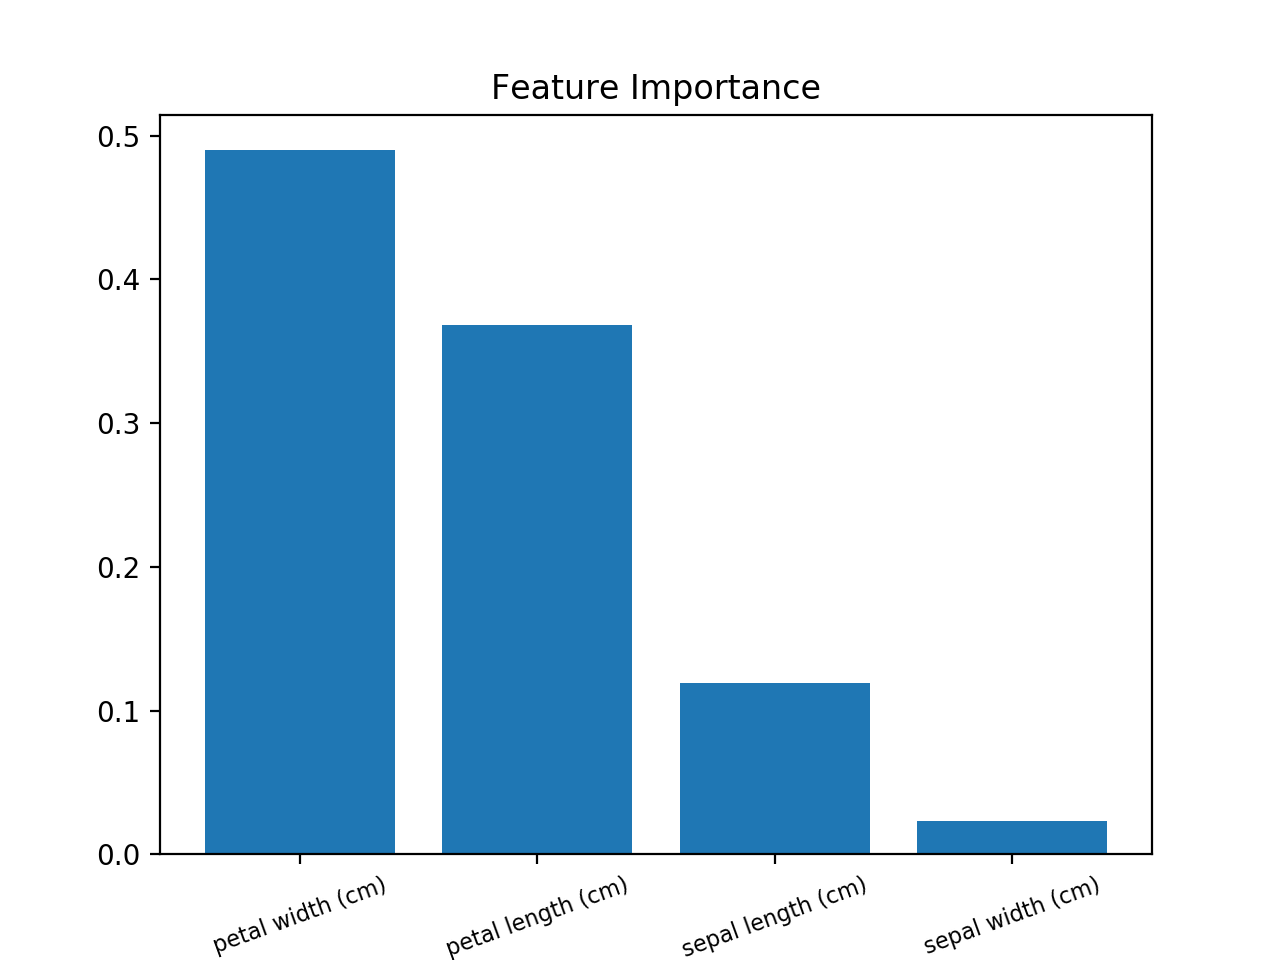
\includegraphics{images/Chapter3/feature_importances_Randomforest.png}
    \caption{RF importances of features used to predict the species of the Iris flower. The y-axis is the relative importance; so a relative importance of $1$ implies the most important and $0$ is the least important feature to predict the species.}
    \label{fig:RF sample FI}
\end{figure}

Random forests are very easily implemented with a two step process with the library \texttt{sklearn} \citep[][]{2011JRFsklearn}.
\section{Multi-layer Perceptrons}
A well known term even amomg non-experts are the words `neural network'.
As the name suggests neural networks are inspired by the network of neurons that make up the mammalian brain.
The basic unit of neural network is a neuron.
A neuron consists of an input, output and an activation function that acts on the input similar to $f(.)$ in Eq~\ref{eq:y=fx}.
This activation function is a mathematical functiom which operates on the input.
Such a unit is called a perceptron and a sample perceptron is depicted in Fig~\ref{fig:perceptron}.
The inputs are combined to form an activation $a_{j}$ via $j$ weights for each input vector value $x_{i}$ making the weight matrix ($w_{ij}$.
The output is defined as ,
\begin{equation}
    y_j = f(\sum_{i=1}^{n} w_{ji}x_i)
    \label{eq: perceptron}
\end{equation}
Many such perceptrons together, producing an output vector $y_{jk}$ for $k$ perceptrons.
This is known as neural network. 
The weights are the neural network parameters whose values can be altered during training.
Activation functions $f(.)$ are typically fixed for the duration of training and varied if the validation results have not reached desirable values.
This is known as a hyper parameter.
The number of neurons in a neural network, the number of weights are also other hyper parameters that can be varied based on the validation results.
The output of a neuron can be treated as an input to another set of perceptrons, and they can be in turn connected to another set of neurons and so on.
Such a network feeds forward the inputs one layer to the next and such networks are called deep neural networks or multi-layer perceptrons.

Based on the kind of combination of $w_{ji}$ and $X_{i}$ perceptron networks can be further sub classified as convolutional neural networks \citep[][]{1990ZhangCNN}, recurrent neural networks and so on.
Neural networks can also work on multi dimensional input as well long vectors.
Configurations of neural networks also vary, for example  other deep neural networks we can also have 

\begin{figure}
    \centering
    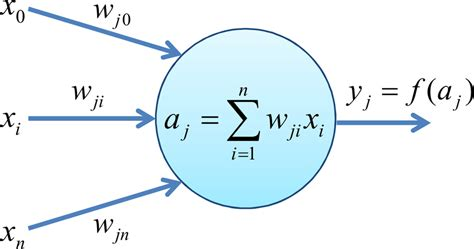
\includegraphics[scale=0.5]{images/Chapter3/perceptron.jpg}
    \caption{A sample percepton consisting of an input vector $X_{i}$ and an output $y$ is depicted here.}
    \label{fig:perceptron}
\end{figure}

\section{Autoencoders}
Autoencoders are special cases of multilayer perceptrons where the input and the output remain fixed but the intermediate layers form a mirrored encoder-decoder structure.
This was first envisioned to denoise data and thus the \citep[denoising autoencoder, ][]{vincent2011connection} was invented.
Typically, the autoencoder has the following main parts,
\begin{itemize}
    \item \textbf{input:} is the input layer which is typically the same shape as the input vector and thus contains as many neurons as the input vector
    \item\textbf{encoder:} the encoder is a set of fully connected neurons which have as input the output of the input layer. 
    These neurons typically are constructed with several layers with the number of neurons in each layer typically reducing in a pyramidal fashion.
    The last layer is the smallest layer and thus the output of this layer is a sparse representation of the input.
    \item\textbf{decoder: } the decoder is a mirror of the encoder both in the layer construction, the number of layers and the neurons used in each layer. 
    It typically terminates in the same number of neurons as the input of the encoder and this layer connects to the output.
    The decoder layer typically reconstructs the input from the sparse representation, thereby recovering a noise free version (note this was the original motivation of the autoencoder).
    \item \textbf{output:} as with the input the output is also a vector equal to the size expected for the output.
\end{itemize}

To wrap this introduction up, we want to make a few points about the limitations of ML algorithms,
\begin{itemize}
    \item \textbf{black box like behavior:} ML algorithms are very useful but also don't particularly lend to great deal of manual fine tuning. 
    Which means that the features that the algorithms learn or not completely controlled and hence to offset this we provide the algorithms with large amount of data.
    \item{\textbf{fine tuning training parameters is challenging:} while there are some thumb rules to follow when training to ensure good training, however there is no way to know if the hyperparameters of the neural network are optimal. 
    Standard techniques such as a parameter space search etc are available but are used when the search itself is not very broad and the parameters have well defined limits}
\end{itemize}

\chapter{Data generation based on a scientific hypothesis}
\label{chap:III.3}
Spectra have a wide range of properties, such as $\rm{SNR}$, line width etc. and we need to choose properties that are in line with science goals of detection and characterization.
The goal of this chapter is to define,
\begin{itemize}
    \item the scientific objective of using spectra with ML algorithms, 
    \item the data that we will use to achieve these objectives and
    \item the metric that will be used to state whether this chosen objective was met or not.
The metric will be common for ML and non-ML algorithms and in principle will be algorithm independent.
\end{itemize}
In that quest we structure this chapter to start with introducing a science goal by defining the detection and characterization hypothesis.
This will then be followed by describing the parameters chosen for data generation followed by a description of the data generation itself.
This will be followed by describing the benchmark metric formulation.
This chapter aims to set up the basic framework that will be used in the two methods chapters in this part.

\section{Scientific goals of using spectral data with ML algorithms}
Using spectra directly with ML algorithms has not been particularly successful for a specific set of characterization problems \citep[e.g,][]{2020Fisher}.
In order to not repeat previous studies and to redefine the goals of spectral data processing with ML algorithms we separate our goals as detection and characterization goals.
Detection goals pertain to identifying that a spectrum indeed contains spectral features that pertain to an exoplanet.
The characterization goals pertain to using the spectral absorption features to derive constraints on the $\rm{T_{eff}}$ and $\log(\rm{g})$ of the exoplanet in the spectrum.
\subsection{Detection hypothesis}
The detection hypothesis is expressed as the ability to identify an exoplanet spectrum when it is extracted from a pixel of a high contrast image based on the features of the extracted spectrum alone.
In the context of high contrast imaging this means that no matter, the contrast of the exoplanet or the resolution of the spectrograph it is possible to make this fundamental distinction based on the spectral absorption features in the spectrum.

This would prove particularly useful when trying to discriminate between speckles and exoplanets in an residual cube.
A well designed algorithm should be able to test and validate this hypothesis.
In this part we will develop a ML and a non-ML based algorithm to test this hypothesis.
We will use the non-ML algorithm to develop the benchmark values that the ML algorithms need to achieve to validate the detection hypothesis.

\subsection{Characterization hypothesis}
The characterization hypothesis is expressed as the ability to constrain physical exoplanetary parameters with a well defined and repeatable error bar when exoplanet spectral features are present in the spectrum.
The exoplanetary parameters that we will consider in my thesis are the $\rm{T_{eff}}$ and $\log(g)$.
In the context of direct imaging data it means that no matter the spectral resolution of the instrument, if exoplanetary spectral features are present in the spectrum then the hypothesis states that we are able to constrain the $\rm{T_{eff}}$ and $\log(\rm{g})$ within the stated error bars. 

This hypothesis is motivated by the idea that it is possible that detection algorithms produce false positives due to their systematic biases. 
However, characterization constraints could allow to rule out such false positives when the detection is marginal.

These two hypotheses form the basis of our data generation, algorithm development and interpretation of those results. 
The detection hypothesis is disproven if we are not able to find (with either the ML or non ML algorithms) the point at which we are not able to make perfect detections no matter the resolution and contrast of the exoplanet present in the spectrum.
The characterization hypothesis is also disproven if we are not able to define the minimum errorbar with which we constrain the $\rm{T_{eff}}$ and $\rm{\log(g)}$.

\section{Data generation to test our hypotheses}
Testing our detection and characterization hypotheses requires us to have data with sufficient variance in data parameters and with sufficient astrophysical variance.
\subsection{ Choice of parameters for data generation}
We confine ourselves to a smaller set of parameters to study we choose three parameters, one of which is entirely intrinsic to the exoplanet we are studying and two of them are intrinsic to the the imaging strategy and the choice of spectrograph.
The parameters we use in this part of the thesis to test our hypotheses are,
 \begin{enumerate}
     \item \textbf{Contrast $\mathbf{C}$:}
     The contrast of an exoplanet is defined as the flux ratio of the mean flux emitted by the exoplanet to mean stellar flux. 
     This is as such regarded as the crucial marker that will allow us detect faint exoplanets. 
     In principle, the brightness of the exoplanet is a free parameter that can vary depending on the temperature, composition, atmosphere physics (such as presence of clouds) and environment of the exoplanet. 
     The brightness of the star is mostly driven by its spectral type and surface gravity.
     Therefore, when the brightness of the star is fixed (by knowning accurately its spectral type and surface gravity), the contrast is only influenced by the brightess of the exoplanet in question.
     \item \textbf{Signal to noise ratio of measured spectrum $\rm{\mathbf{SNR}}$:} number of photons received from the exoplanet vs the instrinsic random noise that is naturally present in the data due to the act of observing an exoplanet.
     This noise is also called photon noise and is usually random in nature.
     This also relates to the quality of the spectrum in that when we have higher number of photons as compared to the number of intrinsic observational noise present in the data.
     The $\rm{SNR}$ is typically a function of integration time of the observations, such that longer observing times lead to higher $\rm{SNR}$.
     \item \textbf{Resolution of the spectrograph $\mathbf{R}$:}
     The spectral resolution is the ratio of fixed wavelength to the difference between wavelengths of two consequent wavelength bins.
     $R$ is typically dependent on the instrument and actually changes with the wavelength in consideration and is typically higher for higher wavelengths.
     To keep the intepretation simple we consider the $R$ as computed for the smallest wavelength in our data.
 \end{enumerate}
These parameters present with a limited exploratory ability, but the choice of the parameters are driven by the detection and characterization seen in the literature.
The $C$ for instance is the single parameter that defines the sensitivity in the data when computing contrast curves. 
The $\rm{SNR}$ is the parameter that is expected to be the limiting factor when developing a new instrument.
The $R$ has long been considered the key factor in using spectra in direct exoplanet detection and \citep[KPIC, ][]{2016Mawet} has prided itself on provide high $\rm{SNR}$ and high $R$ spectra.
\subsection{Synthetic spectra library}
To test our hypotheses, we have chosen parameters that are both related to exoplanet science and instrument engineering.
Ideally, these parameters have to be sampled over a large sample space to ensure that we are able to rigourously test our hypotheses.
Additionally, instrument parameters will require us to have access to instruments with different resolutions but we will need to the exoplanets imaged with these instruments at different $\rm{SNR}$ and $C$.
This also implies that we cannot control the types of noise that are present in instruments and we cannot limit our study to just the observation noise.
Using data from different instruments and different observations will also bring into play,
For example instrument systematics such as the different Strehl ratios produces different amounts of stellar leakages produing variable data.
If we choose just one type of instrument choose to drop $R$ we still risk observation systematics such as different seeing on different nights. 
In addition to other well known effects such as wind halo, these make for a poorly conditioned dataset. 
While in the previous part we sought to verify that our algorithms work with both real and synthetic data, in this part we seek to verify that with working algorithms are our hypotheses valid.

In order to achieve the desired range in the data without taking into account inter-isntrument and site variations, we resort to using synthetic data from the well known templated library, \citep[\textsc{BT-SETTL},][]{1997Allard,2011Allard}.
\textsc{BT-SETTL} conveniently also presents us with a simulation tool \citep[\textsc{PHOENIX},][]{2011Allard} that allows us generate accurate atmospheric spectra by specifying the exoplanet properties.
These models sample the $\rm{T_{eff}}$ range from $1200$K corresponding to warm Jupiter type of exoplanets to $7000$K corresponding to the B supergiant spectral type.
The wavelength range varies from $0.1$ $\mu$m up to $16$ $\mu$m i.e from the infra red to the near visible spectrum. 
This allows to simulate the stellar spectrum and the exoplanet spectrum from the same library.
Using BT-SETTL, we choose a basic grid of models and we generate synthetic from this grid depending on the requirement.
The grid is defined by the following parameters,
\begin{itemize}
    \item[] $\rm{\mathbf{T_{eff}}}$: The exoplanet atmosphere is chosen to be between $1200\le \rm{T_{eff}}\le 1900$ K with a grid sampled every $100$K. 
    This range corresponds to that of warm Jupiters. 
    These temperatures do not lend to very pronounced $\rm{CO}$ emissions, which are quite prominent at higher temperatures which make those templates somewhat easier to detect for cross correlations. 
    The star is chosen to have a $5000\le \rm{T_{eff}}\le 7000$ K surface temperature, the choice of temperature is not so relevant for this problem because beyon a temperature of $4000$ K all of the molecules are fully ionized and the $\rm{T_{eff}}$ only impacts the continuum. 
    In our processing we remove the continuum and hence it does not play a part in the analysis.
    \item []$\rm{\mathbf{log(g)}}$: We choose values for the exoplanet within the existing BT-SETTL model to provide enough range to make an error bar estimate. 
    We choose $2.5\le \rm{\log(g)} \le 5.5$ for the exoplnaet with a grid sampling rate of $0.5$ dex. 
    These $\rm{\log(g)}$s are comnsiderably higher than what we would see for a planet of this type.
    The stellar $\rm{\log(g)} = 2.5$ which is the solar $\rm{\log(g)}$.
    \item []\textbf{Wavelength $\rm{\mathbf{\lambda}}$:} We choose wavelength ranges that allow us to probe the full near infra-red region, $1 \mu\rm{m} \le \lambda \le 3 \mu \rm{m}$.
    This also includes the Telluric absorption lines between $1.78$ and $2.1$ $\mu$m.
    The default spectral resolution of the data $R>300,000$ and the linewidth is in $\AA$. 
    We resample the $R$ as needed but we broaden the line width to match an instrumental profile so that the absorption line widths are realistic.
    We choose this width to be the same as the SINFONI instrumental line width.
\end{itemize}

 \section{Generating synthetic spectra}
We use the \textsc{BT-SETTL} templates to generate synthetic spectra that can be used to test our hypotheses.
Our hypotheses will be tested with both ML algorithms and a cross correlation based non-ML algorithm.
The goal of such testing is to ascertain if a) Which type of algorithm is able to satisfy either or both hypotheses b) what are the constraints we can draw on the algorithms themselves when they are tested.
Consequently, the goals of generating synthetic spectra are also two fold, 
\begin{enumerate}
    \item to be able to explore a parameter space which is relevant from both the astronomical as well as signal processing point of view.
    This will allow us to the test the hypotheses, which are purely based on astronomy, but it will also allow us to understand the interplay between the parameters.
    This is relevant to the community to understand if, of the three parameters we have chosen, are there any which play an important role in validating these hypotheses.
    \item To generate a large number of samples that can be used to train, validate and test the machine learning algorithms that are developed to test our hypotheses.
    In addition to ML algorithms needing a large number of samples to train and generalize well, we also need this parameter space well sampled in order to derive insights into the performance of the ML algorithms on this data.
    As in the case of a cross correlation based algorithm, the community will benefit if we are able to derive the limits at which these hypotheses were satisfied by ML algorithms.
\end{enumerate}
Thus to generate spectra that are astronomically relevant, having realistic observation noise and finally lend to re derivation of the parameters (i.e now they can be viewed as parameters that can be re-estimated by an observer, we generate the same in three steps.
We split the description of this into three subsections, first we create noise-less spectrum from a combination of stellar and exoplanetary spectrum.
We then follow this with explaining the noise injection process and finally we describe the re-derivation of the $\rm{SNR}$ from this noisy spectrum.
\subsection{Creating astronomically accurate synthetic spectrum}
The \textsc{BT-SETTL} template library allows us to choose both the stellar and planetary spectra.
The stellar spectrum is chosen from a grid of $5000\le \rm{T_{eff}} \le 7000$ K with a fixed $\log\rm{(g)} = 2.5$. 
The star in question is randomly chosen as one star in this grid and the flux is measured for every length for this star as $F_{\rm{\lambda,star}}$.
For the exoplanetary spectrum, the exoplanetary template spectrum is randomly chosen with a $1200 \le \rm{T_{eff}} \le 1900$ K and  $2.5 \le \rm{\log(g)}\le  5.5$. 
This random choice thus can have $8$ $\rm{T_{eff}}$ and $5$ $\rm{\log(g)}$ and therefore $40$ combinations.
In practice, to validate our hypotheses, we start with choosing a single template to be our planet.
In the same manner as the stellar spectrum, the exoplanetary planet flux is also measured for every wavelength spectrum as $F_{\rm{\lambda,planet}}$.
Note that both the spectra are chosen from the same library and hence they are both at the same resolution as that of the library. 
They are both first re-sampled to a desired $R$ such that $10^3<R<10^5$.
Re-sampling is a two step process,
\begin{enumerate}
    \item a wavelength vector is first generated with the desired wavelength range where we want to test our hypotheses. 
    In this case we choose $1\le \lambda\le 3$ $\mu$m.
    The $R$ of this wavelength is set to the value we choose to generate our synthetic spectra.
    \item We then interpolate a new synthetic spectrum for the specified wavelength bins based on the flux present in the template library.
\end{enumerate}
This is performed so that both stellar and exoplanetary spectrum are both resampled to the same $R$.
The flux in each wavelength is now based on the initial guess of the physical processes producing the absorption/emission features.
We want to now make sure that every bin has exactly the same relative number of photons so that the sum of all the photons in each of the bins is the same for every spectrum.
Once again to achieve this we have a two step process.
The first of which is normalization.
\paragraph{Normalization:}
Normalization of the flux per wavelength bin ($F_\lambda$) is performed so that the average flux in the spectrum is $1$.
This is expressed as,
\begin{equation}
    F_\lambda = \dfrac{F_\lambda}{\sum\limits_{\lambda} F_{\lambda}}
\end{equation}
Thus, when we do this for the star and its companion we have,
\begin{equation}
    \sum\limits_{\lambda} F_{\rm{planet,\lambda}} = \sum\limits_{\lambda} F_{\rm{star},\lambda} = 1
\end{equation}
Thus both the star and planet are at the same flux. 
The choice of the number of total photons in the spectrum is related to the flux that we are expected to receive at the telescope when observing the spectra.
Therefore, we rescale all the spectra to a specific flux level that is proportional to the $\rm{SNR}$ expected to be recovered.
\paragraph{Scaling the spectra:}
We rescale both the $F_{\rm{\lambda,star}}$ and the $F_{\rm{\lambda,planet}}$ with appropriate flux values.
Starting with the star, we scale the stellar flux as
\begin{equation}
    F_{\rm{star,\lambda,new}} = F_{\rm{star,\lambda,old}}\times\rm{SNR}^2
    \label{eq:scaling of F}
\end{equation}
The exoplanet usually has a total flux that is proportionally scaled to the stellar flux.
Note that while the exoplanet has a blackbody temperature, we concern ourselves only with the reflected stellar flux from the exoplanet.
The absoprtion lines in the exoplanet spectrum are solely due to the presence of specific atmospheric molecules which absorb this reflected light.
The flux from the exoplanet is just a fraction of the stellar flux.
This flux ratio of the exoplanet to the star is $C$.
Thus rescaling the planetary spectra is stated as,
\begin{equation}
    F_{\rm{planet},\lambda,new} = C\times F_{\rm{planet},\lambda,old}\times \rm{SNR}^2
    \label{eq:exoplanet flux}
\end{equation}
where $C\ll1$.
Note that when we compute the rescaled new fluxes of the exoplanet to the star we have,
\begin{equation}
    \dfrac{F_{\rm{planet,\lambda,new}}}{F_{\rm{star,\lambda,new}}} = C
    \label{eq: defn of contrast}
\end{equation}
Thus, the flux of planet to the star defines our contrast as per the definition.
Once the two fluxes have been computed, they have now to be combined and `observed' by a `telescope'.
This act of observation will result in noise, this now the second step to generating synthetic spectra.
\subsection{Noisy spectra generation}
We now have two spectra that have scaled flux values. 
We have yet to combine them to form a single spectrum as in an astronomical observation.
In order to simulate an observation where we extract a spectrum from an observed pixel, we combine both these spectra linearly as,
 \begin{equation}
     F_{\rm{total},\lambda}=(1-C)F_{\rm{star},\lambda,new} + F_{\rm{planet},\lambda,new}
     \label{eq:insertion}
 \end{equation}
Thus, $F_{\rm{otal,\lambda}}$ represents the flux measured at every wavelength bin.
Every wavelength bin now contains stellar and planetary spectral features. 
In terms of the fraction of photons that are present in each bin it is mostly stellar photons as $C<<1$.
Thus now the sum of the total flux in the spectrum can be expressed as,
\begin{equation}
F_{\rm{total}}=\sum\limits_{\lambda}F_{\rm{total,\lambda}}=\rm{SNR}^2 
\label{eq: true signal}
\end{equation}
 This spectrum still does not contain noise, and so the next step is to introduce realistic noise in each wavelength bin. 
 
The act of observing photons arriving at the instrument is equivalent to counting photons.
This results in an intrinsic counting which has a Poisson distribution.
In order to now make this spectrum we replace the photon count in each wavelength bin has a value that is chosen from a Poisson distribution with a Poisson parameter $k$ given by,
 \begin{equation}
     k_\lambda = F_{\rm{total},\lambda}
     \label{eq:noise}
 \end{equation}
This means that the flux distribution for each bin is given by,
 \begin{equation}
    \textrm{PMF}(k_\lambda) = \mu^{k_\lambda}\dfrac{\exp(-\mu)}{k_\lambda!} 
    \label{eq: poisson}
 \end{equation}
A random value is chosen from this PMF, this random value will now represent the signal such that,
 \begin{equation}
     F_{\rm{noisy,\lambda}} = \textrm{random}\left(\textrm{PMF}(F_{\rm{total,\lambda}})\right)
 \end{equation}
In practice both of these equations are easily replicated with the \textsc{numpy.random} function of \textsc{poisson}.
Note that this function has to be applied repeatedly over every wavelength bin.
This is now, one realization of a noisy spectrum.
When this repeated many times with many number of spectra we will have spectra each having its own noise realization. 
This is the final step in generating the synthetic spectrum.

The spectra that we have calculated now are generated using a specific $R$ where the exoplanet spectrum is computed with a mean contrast $C$. 
We have produced these exoplanets with a known flux such that the final $\rm{SNR}$ is fixed for these spectra.
These three parameters will be uniquely populated for each spectrum that we produce using this method.
In the next subsection we will examine how the $\rm{SNR}$ is based on the initial flux we inserted.
\subsection{Computing the $\rm{SNR}$ from the noisy spectrum.}
In order to compute the $\rm{SNR}$ of the spectrum we  first need to reliably measure noise. 
An advantage of using purely synthetic data is that we are able to precisely quantify the noise, which can then be used to compute the signal to noise of the cross correlation and the spectra.
In the following section we will discuss how we use the noise computed in the spectra to compute the signal to noise of the cross correlation as well.
To start with we compute the amount of noise that is inserted in each wavelength bin.
The precise expression of noise in any wavelength bin is 
\begin{equation}
    N_\lambda = F_{\rm{noisy,\lambda}}- F_{\rm{total,\lambda}}
\end{equation}
The per bin noise is the one that follows Poisson statistics and therefore, it is the standard deviation of this noise that allows us to estimate the true noise in the spectrum.
The standard deviation of the noise for $N$ wavelengths in the spectrum is expressed thus,
\begin{equation}
    \sigma = \sqrt{\dfrac{1}{\rm{N}}\sum\limits_{\lambda}\left(N_\lambda-
    \dfrac{1}{N}\sum\limits_{\lambda} N_{\lambda}\right)^2}
    \label{eq:std of noise}
\end{equation}
$\sigma$ is now a generalized measure of the noise that is inserted in the spectrum.
The signal inserted in the spectrum is given by Eq~(\ref{eq: true signal}).
Thus we have a true generalize measure of the noise in Eq(\ref{eq:std of noise} and the signal.
This can then be turned into a $\rm{SNR}$.
This $\rm{SNR}$ now will refer to the signal to noise ratio of the spectrum. 
The noise that we produced is a bin-to-bin noise and therefore over a large number of bins the mean of the noise will reduce to $0$ and so Eq~(\ref{eq:std of noise}) can now be rewritten as,
\begin{equation}
    \sigma = \sqrt{\dfrac{1}{N}\sum\limits_\lambda N^2_\lambda}
\end{equation}
and because of the properties of a Poisson distribution, we can simplify the standard deviation of the noise in the spectrum as,
\begin{eqnarray}
    \sqrt{\dfrac{1}{N}\sum\limits_\lambda N^2_\lambda}&= \rm{SNR}\\
    \therefore \sigma &= \rm{SNR}
\end{eqnarray}
Consequently, we can now express the signal to noise of the spectrum as,
\begin{equation}
   \dfrac{\sum\limits_{\lambda}F_{\rm{total,\lambda}}}{\sigma}=\rm{\dfrac{SNR^2}{SNR}= SNR }
\end{equation}
In other words, starting from the initial flux that we set in the spectrum we can derive the final signal and noise with just two equations,
\begin{eqnarray}
    \rm{signal} &= \sum\limits_{\lambda}F_{\rm{total}}\\
    \rm{noise} &= \sqrt{\sum\limits_{\lambda}F_{\rm{total}}}\\
\end{eqnarray}
Thus, we have a simulation method that starts from a synthetic spectra library and produces exoplanet spectra that can be used to test our hypotheses.
These spectra can in principle be sampled over an infinite range of parameter space other than computational limitations placed on $R$ because of the size of the vectors.
This also allows us to explore the extent of detection and characterization that will form a complete test of our hypotheses.
As a next step, we will need to define a benchmark on which we can test our hypotheses.

%This spectrum is subject to some basic pre-processing in line with \cite{haffert2019} to remove stellar features and then fed into the CCF pipeline.
%explain this in the methods chapter.

\section{Developing a common benchmark for ML algorithms and non-ML algorithms}
A common benchmark is particularly challenging define for this part of my thesis because there are three cornerstones that need to be satisfied.
The three cornerstones would be performance of the algorithm independent of the science goals, benchmark for the detection hypothesis and benchmark of the characterization hypothesis.
All of the algorithms developed in this part of the thesis have to be tested through each of these benchmarks. 
To begin with each algorithm is evaluated for its performance through evaluation benchmark, when this benchmark is reached for the algorithm then it will be used to test the detection and characterization hypotheses.
The goal of this exercise is to understand two things,
\begin{enumerate}
    \item An algorithm could be well defined and developed (in the case of ML algorithms well trained) but does it pass the basic benchmark to be used in scientific data processing
    \item what are the limits that the algorithm places on the scientific hypotheses given that that the algorithms passes the basic performance measures.
\end{enumerate}
Finally, the end goal of this benchmarking procedure is to understand the strengths and limitations of the algorithms developed for this part
\subsection{ Evaluation of the algorithms through confusion matrices}
As defined, in our synthetic data we are able to full range of parameters. 
Once we have developed our algorithm, we will evaluate this algorithm on a specific range of parameters.
We will define th $\rm{min}$ and $\rm{max}$ of these parameters when evaluating the  algorithm.
The basic test of this algorithm development is to be able to use the absorption features unique to the exoplanet spectrum, distinct from the steallar emissions and other noisy variations in the spectrum.
The fundamental test is therefore, to define limits of the output of the algorithm such that we can be convinced that this algoritm does not get confused between spectra that contain no such exoplanetary features and those that contain them.
While, we evaluate the algorithms independently, we impose constraints that will allow us to evaluate the limits of scientific data processing fairly.
One of the constraints is the false positive rate of a detection and/or characterization algorithm cannot be higher than $10^{-4}$.
Since we define characterization as the $\rm{T_{efF}}$ and $\rm{\log(g)}$ of the exoplanet inferred from its absorption lines, a false positive would be a mis-recognition of the presence of such absoption lines and indeed inferring an non-existent value for these parameters.

This benchmark has to also be shared by both ML and non ML algorithms. 
The benchmark also has to allow us to evaluate the false positives produced by algorithms while also changing the threshold. 
Therefore, a well designed benchmark that is consistently used is confusion matrix.
The confusion matrix allows the evaluation of false positives and true positives in the data for a specific output from the algorithm.
In this part we will define a true a positive as when a synthetic spectrum contains the spectral features of an exoplanet and the algorithm has correctly identified this spectrum as such.
A false positive is defined as when a spectrum does not contain an exoplanetary spectrum i.e when $C=0$ in Eq~\ref{eq:insertion} but the algorithm indentifies this as a spectrum that contains exoplanetery features.
A sample confusion matrix is given in Tab~\ref{tab:sample_cm}. 
The confusion matrix rows are two different conditions which will be applied to Eq~\ref{eq:insertion}.
The condition where $C=0$ is the case where pure stellar spectra are evaluated by the algorithm and the number of such spectra which are correctly inferred as no exoplanet being present are counted.
Note that the algorithms are subject to thresholds which will allow us to count the spectra which produce above or below a fixed threhold so that this matrix can be computed.
\begin{table}[ht!]
    \centering
    \begin{tabular}{|c|c|c|}
    \hline
    Condition&  \multicolumn{2}{|c|}{ Predictions}\\
    \hline
        $C>0$ &\cellcolor{green!50}  True positives& \cellcolor{red!50}False negatives\\
        \hline
        $C=0$ &  \cellcolor{red!50}False positives& \cellcolor{green!50}True negatives\\
        \hline
    \end{tabular}
    \caption{A sample confusion matrix that is the benchmark that is used to evalute the algorithm in consideration. 
    The cells in green are values that the algorithm needs to correctly predict and those in red are those parameters that the algorithm makes mistakes on.
    The False positives have to be limited to $10^{-4}\le$ whereas we don't put any constraint on the False negatives.}
    \label{tab:sample_cm}
\end{table}
The goal of this confusion matrix is to evaluate the performance of the algorihm purely as a signal processing tool with some constraints defined by the final scientific goals. 
Since cross correlation based algorithms are fairly well tested, it is somewhat moot to test them with this method however, this is very important to understand if the performance of the ML algorithms compares to the cross correlation algorithm as a signal processing tool.
The confusion matrices will have to be evaluated for different ranges of the parameters and a good algorithm will perform similarly for different ranges or have very well quantifiable limits for the value of $C$.
\subsection{Quantifying the algorithm as a detection tool}
Once an algorithm passes the test of individual confusion matrices, it is important to test what are the limits of our detection hypothesis. 
The detection hypothesis can be fully or partially satisfied where the detection is possible given some constraints on the data.
This needs to be clearly quantified as we vary the parameter space and it also needs to be quantified as a function of different parameters.
In order to fully realize the detection limits of the algorithm, we propose a detection matrix in this thesis that evaluates the detectability of a warm Jupiter across different $R$ and $\rm{SNR}$.
Such a detection matrix using the data defined in this section is useful for the following reasons,
\begin{enumerate}
    \item Define the intrinsic detectability of warm Jupiters as a function of instrument resolution and observation signal to noise
    \item define the minimum contrast at which a fixed instrument resolution allows us to detect a warm Jupiter. 
    \item Given a contrast of a candidate exoplanet, the detection matrix should serve to define the minimum $\rm{SNR}$ of an observation.
\end{enumerate}
The advantage of having such a detection matrix in addition to quantifying intrinsic detectability of an exoplanet is to be able to compare different algorithms that operate on spectra.
While this matrix is meant to offer insight into the type of observation and instrument to be used to detect an exoplanet type, it can also be used to quantify the best algorithm to be used for this combination as well.

The detection matrix comprises of three components, the rows the columns and the values inside the cells.
From the bottom to the top the rows represent increasing $\rm{SNR}$ with the maximum $\rm{SNR}$ forming the last row.
The columns represent increasing spectral resolution with the highest resolution as the last column.
Thus, each cell is indexed by an observing and instrument parameter.
Both there parameters define the spectral properties unique to that observation carried out with the instrument and will therefore, using our algorithm, set a detection limit to the exoplanet.
We will define this detection limit as the maximum contrast that the exoplanet is detectable at. 
A sample of such a matrix is shown in Tab~\ref{tab:sample_detmat}.
\begin{table}[!ht]
    \centering
    \begin{tabular}{||c|c|c|c|c||}
    \hline
    \hline
         {$\rm{SNR}$ of the observation}& \multicolumn{4}{c}{Resolution of the instrument}\\
         \hline
                  &  $R_1$              &$R_2$        &..&$R_n$\\
         \hline
         $\rm{SNR_1}$&$C_{R_1,\rm{SNR_1}}$&$C_{R_2,\rm{SNR_1}}$&..&$C_{R_n,\rm{SNR}_1}$\\
         \hline
         $\rm{SNR_{2}}$&$C_{R_1,\rm{SNR_2}}$&$C_{R_2,\rm{SNR_2}}$&$..$& $C_{R_n,\rm{SNR_2}}$\\
         
                ..  & .. &.. &  .. &..    \\ 
                ..    & ..  &.. &  .. &..    \\ 
                ..    & .. &.. &  .. &..    \\ 
                    \hline
        $\rm{SNR}_n$&$C_{R_1,\rm{SNR}_n}$&$C_{R_2,\rm{SNR}_n}$&..&$C_{R_n,\rm{SNR}_n}$\\
         \hline
         \hline
    \end{tabular}
    \caption{Sample detection matrix where the rows represent a different $\rm{SNR}$ numbered from $1$ to $n$ where $\rm{SNR_1}$ represents the spectrum with the highest $\rm{SNR}$.
    Columns are indexed by the wavelength resolution of the spectra that are processed by the algorithm.
    Each entry correesponds to the contrast at which the algorithm is able to detect the exoplanet observed with its correspoding $\rm{SNR}$ amd $R$.
    Thus a contrast $C_{R_1,\rm{SNR}_1}$ corresponds to the contrast at which the exoplanet can be detected when observed with a $\rm{SNR_1}$ and a resolution $R_1$ and so on.}
    \label{tab:sample_detmat}
\end{table}
The detection matrix depicted above has rows indexed by the $\rm{SNR_1}$ to $\rm{SNR}_n$ which represents signal to noise values that differense spectra are generated with. 
In this example the maximum $\rm{SNR}=\rm{SNR}_1$ and the minimum would be $\rm{SNR}_n$. 
Similarly, the columns are indexed by the spectral resolutions ranging from $R_1$ to $R_n$ where $R_1$ is the smallest resolution and $R_n$ would be the spectra with the highest resolution.
Each entry of the detection matrix is indexed with a $C_{R,\rm{SNR}}$ which is the contrast at which the exoplanet is detected when synthesized with a $\rm{SNR}$ and $R$.
There is no preferential ordering to the contrast, however, the detection matrix allows us to get an intuition of how deep a contrast is detectable with increasing $\rm{SNR}$ as we traverse from the bottom most row to the topmost with the same $R$.
Similarly we can infer the detectable contrast evolution with changing $R$ from left to right along the columns.
\subsection{Quantifying the characterization hypothesis using the characterization matrix}
As described earlier, spectral features such as molecular absorption lines are impacted by the $\rm{T_{eff}}$ and the surface gravity ($\rm{\log(g)}$) of the exoplanet.
Therefore, a benefit of having algorithms that process spectra to detect exoplanets also allows us to draw inferences about these parameters that produce these spectra.
The characterization hypothesis states that it is possible to characterize an exoplanet \textit{provided} that exoplanetary features are indeed present in the spectra.
As stated earlier, the goal of the characterization using the $\rm{T_{eff}}$ and $\rm{\log(g)}$ was to also rule out false positives where a detection could be claimed but we could infer this as a false positive based on the characterization of the spectrum.
This is where the characterization matrix comes into play.
The characterization matrix needs to perform the following actions,
\begin{enumerate}
    \item quantify the relative strengths of the presence of absorption features for different templates using both ML and non-ML algorithms.
    \item Using this quantification, the characterization matrix should be used to derive the error-bars on both $\rm{T_{eff}}$ and $\rm{\log(g)}$ and
    \item finally visually the characterization matrix should provide clear evidence that there is preferred combination of $\rm{T_{eff}}$ and $\rm{\log(g)}$.
\end{enumerate}
The last point is fairly important when comparing a large number of spectra and its matrices, where unlike the detection matrix, the characterization matrix has to lend to quick perusal and acceptance.

This matrix will take a similar shape to the matrix in \textcolor{blue}{[Refer to Part II Methods chapter]}. 
We used multiple templates there to justify the best template to be used in the case of HD142527b \textcolor{blue}{[Refer to Part II Results HD142527b]} and conversely showed that the template does not make any impact on PDS70 \textcolor{blue}{[Refer to Part II Results, PDS70]}.
In that case we used the matrix purely as a visual and qualitative justification for the use of the templates to produce maps of the detected companion.
In order to fulfil the quantitative criteria we will go on to use the change of the output of the algorithm for different templates.
The dispersion of the changw will allow us to quantify the error in $\rm{T_{eFF}}$ and $\rm{\log(g)}$.
There are two basic reasons to use the dispersion of the detection parameter across different templates,
\begin{enumerate}
    \item this dispersion of the detection parameter allows to constrain the sensitivity of the algorithm to supplying the closest template to the exoplanet present in the spectrum.
    \item constrain the sensitivity of both $\rm{T_{efF}}$ and $\rm{\log(g)}$ to varying templates.
\end{enumerate}
Note that it is possible to produce this characterization matrix when there is sufficient evidence that the algorithm is indeed sensitive to changing templates.
It is outside the scope of the thesis to define another metric for this 'sensitivity' but tests with different templates in one of the metrics defined here have to give us the confidence that the algorithm is indeed sensitive to changing templates.
In the subsequent sections we will discuss the application of this benchmark to both ML and non-ML algorithms and the results produced therein.


\chapter{Performance of cross correlation based algorithm on the benchmarking metric}
\label{chap:III.4}
In this part we have developed two classes of algorithms, non-ML based algorithms and the ML based algorithms.
This chapter deals with the non-ML algorithms that were developed to use spectra to test our hypotheses.
Primarily, we use cross correlations to perform the bulk of our processing in the non-ML algorithm.
The algorithm consists of the following broad steps, each of which will be described in the methods,
\begin{enumerate}
    \item Subtraction of the stellar template from the spectrum produced in Eq~\ref{eq:insertion} and initial pre-processing similar to \textcolor{blue}{[Refer to Part II Methods, pre-processing]}
    \item Computation of the cross correlation using the basic equation Eq~\textcolor{blue}{[Refer to Part II Methods,cross correlation]}, but with a different velocity dispersion,
    \item computation of the detection and characterization parameters as is appropriate and 
    \item finally, produce the detection and characterization matrices from these parameters.
\end{enumerate}
We will then present the results of this algorithm with different inputs and explore the parameter space in the results section.
We will end this chapter with the criteria that ML algorithms will need to satisfy in order to be considered one of the following,
\begin{itemize}
    \item better than the ML algorithms and therefore would have validated both hypotheses,
    \item as good as the ML algorithms but need not have validated both hypotheses but at least one of them,
    \item worse than the ML algorithms and therefore not considered appropriate to proceed to validating the hypotheses.
\end{itemize}
The goal of this chapter is thus to summarize the functioning of a basic algorithm that uses cross correlations, but also is able to produce scientifically relevant results.
This also serves as the basis on which to evaluate the ML algorithms.

\section{Methods}
The cross correlation based non ML algorithm takes as input the spectrum resulting from Eq~\ref{eq:insertion}.
The output is available at different steps in the algorithm and can be used for diverse purposes at each step,
\begin{enumerate}
    \item at the end of the pre-processing step we will have spectra which are deconvolved from stellar features and are continuum subtracted. Normally, this is the spectrum that has to be cross correlated with the template, but this can also be used for other characterization purposes where the contiuum does not form the basis for characterization,
    \item at the end of the cross correlation, we get the cross correlation coefficients at different velocity dispersions between the template and the input spectrum. 
    This non-normalized but can used to get an idea of what similarity between spectra are.
    \item Finally, the detection and characterization parameters are the cross correlation signal to noise and the log-likelihood of the templates which can also be used to produce log-likelihood based characterizations.
\end{enumerate}
\subsection{Pre-processing and cross correlation}
The pre-processing of the spectra is in line pre-processing that was described in \textcolor{blue}{[Refer to Part II, Methods, pre-processing]}.
In the case where we have image data we have the advantage of knowing the pixels where the star is present, therefore we measure the exact stellar spectrum.
This also has the effect of measuring noisy stellar spectrum and therefore when subtracting the stellar spectrum could mis-subtract the noise.
There has been some evidence where stellar spectra from templates are used \textcolor{green}{[Include this citation]} to model the stellar spectrum to deconvolve it from the measured spectrum.

In this case, since our data is purely synthetic, we use the known stellar spectrum to divide out stellar features.
In order to do this we undertake the following steps,
\begin{enumerate}
    \item We compute the sum of the stellar spectrum in Eq~\ref{eq:scaling of F}. This would be the total flux that the spectrum has been normalized to and then divide the final spectrum generated in Eq~\ref{eq:insertion} by this value.
    \item This is followed by computing computing the reference spectrum from the scaled stellar spectrum by applying a Savitzky-Golay filter of order $1$ and window size $101$ on the normalized stellar spectrum.
    This is the reference spectrum.
    \item Finally, the reference stellar spectrum is divided out of every synthetic spectrum.
\end{enumerate}
This leaves a continuum free spectrum, as in \textcolor{blue}{[Cite Part II, Methods, pre-processing]}.
But the noise in the spectrum and the exoplanet spectrum and its contrast remain unaltered.

The next step is cross correlate this spectrum with a template spectrum and produce a cross correlation vector for different velocity dispersions.
As with \textcolor{blue}{[Refer to Part II Methods, cross correlation]} we use Eq~\textcolor{blue}{[Refer to Part II methods, cross correlation equation]} to cross correlate a chosen template spectrum with the target spectrum.
In \textcolor{blue}{Part II cross correlation} we used a large velocity dispersion of $-2000$ to $2000$ km/s between the spectra and use the larger velocity dispersions as the noise computation baseline.
We saw that this large range of dispersions are computationally expensive but provide signal to noise values for each pixel.
The reason of doing so in the previous part was the lack of a standardized technique to measure noise in the data.
In this Part the data we use is purely synthetic and hence the noise is well measured.
We also don't introduce a relative velocity shift between the template and the target spectrum.
Thus, if there is a match between the template and the target then it will be present at $v=0$ km/s.
But in order to be still considered a cross correlation we still provide a small velocity dispersion to work with.
Consequently, the velocity dispersion we choose is between $-50$ to $50$ km/s.
The velocity resolution of this cross correlation is related to spectral resolution as,
\begin{equation}
    \delta v = \dfrac{V_{1}}{R}
\end{equation}
where $\delta v$ is the velocity resolution and $V_1$ is the velocity at $1$ km/s.
Finally, we will recompose the cross correlation vector to now be used to produce both the detection and the characterization parameters.
\subsection{Development of the detection parameters and its application}
Claiming a detection in the field of exoplanet detection is probably one of the most contentious issues in the field.
As we have seen in \textcolor{blue}{[Refer Part II methods, SNR]} it is possible to use signal to noise from the cross correlation to define a detection threshold.
However, computing this signal to noise ratio is computationally intensive and does not take into account the auto-correlation. 
In this part we will re-compute the signal to noise of the cross correlation by taking into account the auto correlation and taking the noisiness of the spectrum into account.

To begin with we define the `signal' of the signal to noise which is defined as,
\begin{equation}
    S(0) = CC(0)
    \label{eq:numerator-snr}
\end{equation}
where $CC(0)$ is the cross correlation value at $v=0$ and therefore this is the signal at $v=0$. 
This follows from the cross correlation value defined in \textcolor{blue}{[Refer Part II cross correlation]}
It is possible to generalize this for different velocities but this generalization is out of the scope pf this thesis.
The `noise'  comprises of two quantities, the noise measured of the spectrum $\sigma$ and the auto-correlation value.
The auto-correlation value is defined as in the cross correlation function as follows,
\begin{equation}
    \textrm{AC}(v) = \sum\limits_{\lambda}M_{\rm{\lambda}}\times (M_{v,\lambda}-M_{\textrm{SG},v,\lambda})  
    \label{eq: AC equation}
\end{equation}
where $\textrm{AC}(v)$ is the auto correlation value at $v$, as before $M_{\lambda}$ is the model flux in wavelength bin $\lambda$ and when the $v$ suffix is added it is the wavelength shifted version by a velocity dispersion $v$.
The $M_{\textrm{SG},v,\lambda}$ is the Savitzky-Golay filtered version of the template.
Note that this also acts as mean subtraction for the second term while the first term is used as is.\textcolor{red}{[The goal is to keep the first term pristine and untouched whereas the second term is the "template". Not sure if I need to state that here.]}
Thus now we have the noise terms namely the noise ($\sigma$) and the auto-correlation $\textrm{AC}(v)$.
We use these three terms to compute a signal to noise value for each cross correlation.
We define the cross correlation $\rm{SNR}$ only for $v=0$ and is denoted as $\rm{SNR_{ccf}}$ .
We then compose the noise portion of this signal to noise thus,
\begin{equation}
    N(0) = \sigma \sqrt{\textrm{AC}(0)}
\end{equation}
A key point to be noted is that the effect of the auto-correlation as a noise term is considered only a square root, while the full value of $\sigma$ is considered.
Therefore, when the auto-correlation increases its effect is not increased in an unbound manner, which if allowed could have allowed this effect to overwhelm the effect of the noise.
As with the signal we compute the noise at $v=0$.
The next step is to use both these parts to compose the signal to noise metric.

Claiming a detection is fraught with difficulties particularly when doing so with $\rm{SNR_{ccf}}$.
While other $\rm{SNR}$ techniques such as \cite{2014MawetSNR} has been well whetted and their limitations are well understood \citep[e.g STIM][]{2019Pairet}, there is very little literature on the robustness of calculating $\rm{SNR_{ccf}}$.
Therefore, when thresholding such measures, there is very little understanding of what the false positive rate is at different thresholds.
But a threshold we must set and a threshold we will have.
A contribution of this study is to also estimate the false positive rate at a threshold of $\rm{SNR_{ccf}}\ge 6$.
Note that this signal to noise ratio is still just a metric of the similarity between the target spectrum and its template and not a significance of the detection.
%The CCF algorithm performs the cross correlations and returns a $\rm{SNR_{ccf}}$ using the formula from \cite{ruffio2019radial},
Finally, we use the expression in \cite{ruffio2019radial} to compute the cross correlation signal to noise as follows,
\begin{equation}
    \rm{SNR_{ccf}}=\frac{CC(0)}{\sigma \sqrt{\textrm{AC}(0)}}
    \label{eq:ccf-snr}
\end{equation}
In order to make this a detection parameter we take the following steps,
\begin{enumerate}
    \item we generate several synthetic spectra with a fixed $R$ and $\rm{SNR}$,
    \item then we cross correlate these spectra with a template of choice. In order to not be very optimistic in estimating the sensitivity of this technique we choose a spectrum that is a $1$ grid point both in $\rm{T_{eff}}$ and $\rm{\log(g)}$ away from the synthetic spectrum exoplanetary template to act as the template.
    \item Finally we compute the $\rm{SNR_{ccf}}$ for each spectrum. We then choose as the limiting contrast the contrast at which $\rm{SNR_{ccf}}-6$ is the lowest positive value.
    We repeat this experiment $100$ times and compute the mean contrast with $100$ repetitions to avoid any random effects.
    \item We fill the value of contrast in the detection matrix to form the detection parameter for the $R,\rm{SNR}$ combination.
\end{enumerate}

\subsection{Development of the characterization parameter and its application}
The cross correlation coefficient is a measure of similarity between a template spectrum and the target spectrum.
The extent of this similarity is quantified by $\rm{SNR_{ccf}}$.
However, while this is a measure of the similarity, there is not much evidence to show that it is a good measure of the \textit{difference} between spectra.
The characterization parameter needs to encapsulate the following pieces of information,
\begin{enumerate}
    \item the extent of similarity of one template (within the characterization parameter space as discussed in the previous chapter) with the target spectrum,
    \item the relative non-similarity of other templates with the target spectrum and this will allow us to quantify the difference between individual templates and identify the spectrum that best fits with the exoplanetary template in the synthetic spectrum.
\end{enumerate}
Thus, characterization is an exercise in optimizing the parameter space such that the optimal value of the characterization parameter can be defined.
We use log-likelihood of the cross correlation to evaluate the optimal combination of $\rm{T_{eff}}$ and $\rm{\log(g)}$ and measure the uncertainty in estimating this value.
In this subsection we describe our derivation and use of the characterization parameter by answering three fundamental questions, a) What is the advantage of log-likelihood b) how do we define the relationship between cross correlation and log-likelihood and finally c) how do we use the properties of this log-likelihood to derive the error bars of the characterization of an exoplanet.

\paragraph{Why do we need a log-likelihood at all?\\}
The idea of using log-likelihood as a method to estimate parameters inferred from cross correlations was first introduced by \cite{2003Zucker} who derived one of the earliest cross correlation to log-likelihood expressed as,
\begin{equation}
    LL \propto \log(1-\rm{CC}^2)
    \label{eq:LL-cc eqn}
\end{equation}
The goal of such an log-likelihood was to have a $\chi^2$ like behaviour, the standard deviation of which can be used to compute the uncertainty.
As justified in \cite{2019Brogi}, the use of the negative sign and the dependence on the square of the cross correlation allows for two crucial factors to be considered,
\begin{enumerate}
\item using the square of $\rm{CC}$ will allow us to make a deep likelihood trough only for truly high cross correlation values and any small variations will get ruled out.
This will allow us to fit an inverted Gaussian and derive the uncertainty.
\item The negative sign enables to only have true cross correlations of absorption features to absorption features to produce a strong $LL$,
This in turn will let us ensure that the best matching template is the one that truly matches the features of the template to its noisy equivalent.
    \end{enumerate}
Hence, the use of $LL$ and cross correlations was deemed appropriate.

\paragraph{How do we adapt this concept to our specific case?\\}

Eq~\ref{eq:LL-cc eqn} conceptually defines the relationship between the cross correlation and the log likelihood. 
However, we still need to take two aspects into consideration when it comes to synthetic data as discussed in \cite{2019Brogi},
\begin{enumerate}
    \item the nature of the noise. In this case the noise distribution is random with no intrinsic structure to the noise in each bin. Therefore, we can consider $\sigma$ to be the noise used for $LL$ as well.
    \item The effect of the stellar continuum, which has been removed by mean subtraction.
\end{enumerate}
Therefore, we can go about using the derivation of the log-likelihood as described in \cite{ruffio2019radial},
\begin{equation}
LL \propto -\dfrac{\dfrac{CC^2}{\sigma^4}}{\dfrac{AC}{\sigma^2}}
\end{equation}
This equation can now be simplified and the proportionality turned into an equality by using a scaling constant $a$, as
 While the SNR is derived from Eq(\ref{eq:snr}), the LL is computed based on \cite{ruffio2019radial} as,
 \begin{equation}
     \rm{LL}=-a\rm{\frac{CC^2}{\sigma^{2}AC}}
\end{equation}
This constant of proportionality is related to the mean continuum energy present in the spectrum and \cite{2003Zucker} shows that this constant can be set $a=1$ for the two conditions of continuum and mean subtraction.
Thus, we have the final $LL$ computation is giveny by,
 \begin{equation}
     \rm{LL}=-\rm{\frac{CC^2}{\sigma^{2}AC}}
     %-\frac{(\frac{CCF}{\sigma^{2}})^{2}}{\frac{ACF}{\sigma^{2}}}
     \label{eq:LL}
 \end{equation}

\paragraph{How do we use this log-likelihood to compute the uncertainties?\\}

As stated earlier this log-likelihood function takes on a $\chi^2$ shape around the template library parameter space which can be used to infer the uncertainties. 
The characterization matrix consists of rows of $T_{\rm{eff}}$ and columns of $\rm{\log(g)}$ and we fill each cell with the $LL$ computed using the spectrum with the corresponding combination of rows and columns.
This results in 2D matrix, however the error bars have to be computed separately in $\rm{T_{eff}}$ and $\rm{\log(g)}$.
In order to now compute the error bars separately, we first find the cell with the lowest value of $LL$.
This is the initial guess of the parameters that we supply to the inverse Gaussian fit.
Then we fit an inverse Gaussian as defined by,
\begin{equation}
    LL_{g} = \dfrac{A}{\sigma_{x}\sqrt{2\pi}}\exp{\left(-\dfrac{(x-\mu_x)^2}{2\sigma_{x}^2}\right)}
    \label{eq: gaussian fit LL}
\end{equation}
where $LL_g$ is the inverse Gaussian we fit to the $LL$, $x$ is the parameter we are guessing i.e either $\rm{T_{eff}}$ or $\rm{\log(g)}$,
$\mu_x$ and $\sigma_x$ are the mean and standard deviation of the Gaussian fit.
These represent the estimated value of the parameter and our desired error bar.
As guesses we have to specify th starting value of the parameter, we first start with a guess value of $T_{eff}$ or $\rm{\log(g)}$ at the lowest value cell and for the $\sigma_x$ we choose the desired error bar.

\section{Results}
This results section will discuss the results of the cross correlation based algorithm from a scientific point of view.
It has been stated that for both the ML and non-ML algorithms, the confusion matrices for each algorithm will be computed for specified parameter space. 
While this is useful to evaluate the algorithm, it does not make statement about the detection and characterization of exoplanets.
Therefore, the description of the confusion matrix of the cross correlation algorithms will be discussed in \S\ref{chap:II.5}.
In this section we will discuss the following aspects,
\begin{enumerate}
    \item the parameter space that was used to generate these experiments and how the cross correlation fares in this parameter space. We will describe the scientific motivation of this parameter space, 
    \item this is followed by the description of the detection matrix and a brief discussion of what the discussion matrix means for scientific data processing and
    \item finally, we will describe the error bars which we were able to compute using the characterization matrix.
\end{enumerate}
We will wrap this section with implications that these results mean for the scientific community in general.
\subsection{The parameter space that we use to generate data}
As a reminder, the parameter space here is the range of values we supply for the contrast ($C$), the instrument resolution $R$ and the spectral signal to noise ratio ($\rm{SNR}$).
Each of these parameters have different consequences for the science, the instrument selection and finally observation baseline duration.
It is not possible to practically cover every scenario but a good choice of the parameter space selection would be to cover as wide a net as possible for the parameters in question.
Alternatively, we could choose to define limits to the parameters which will have scientific relevance.
Before we describe the choice of parameters we must first define what is the "sampling" criteria for these parameters.
Due to the advantage of using synthetic data, we can freely define our sampling criterion and thereby have as fine a mesh as needed.
The sampling criteria has both storage and computation time consequence particularly if we vary these parameters simultaneously.
The parameters $C$ and $\rm{SNR}$ do not have any additional computational requirements when they are changed, however, $R$ has increasing computational constraints.
$R$ is directly proportional to the total number of wavelength bins in the data, 
\begin{equation}
    \rm{N}\approx 2R
\end{equation}
where $N$ is the total number of wavelength bins in the data. 
While this relationship changes slightly and the constant of proportionality ($2$) rises with increasing $R$ it will still remain between $2$ and $2.5$.
Therefore, when we generate the parameter space the computational costs of computing cross correlations are significantly higher at higher resolutions.
This will become pertinent when using ML algorithms, but for the purposes of this chapter the only limit on the value of $R$ is the resolution limit of the template library.

\paragraph{Parameter ranges of $C$:\\}
Contrast is defined in the Eq~\ref{eq: defn of contrast}.
This contrast varies over each wavelength bin such that different wavelength bins have varying contrasts.
However, when referring to contrasts, we will always refer to the mean contrast of the spectrum.
The contrasts we choose lie on a logarithmic scale between $C_{\{rm{min}}$ and $C_{\rm{max}}$.
We choose the $C_{\rm{min}}=10^{-2}$ based on the contrasts of HD142527b which has been detected well by the cross correlation algorithm \textcolor{blue}{[Refer to Part II Results, HD142527]}.
The choice of $C_{\rm{max}}$ based on the detection limits set the warm Jupiter \citep[\textsc{1000246b}][]{2015Quanz,2023Cugno} with a contrast of between $10^{-5}$ and $10^{-6}$.
Thus with the $C_{min}$ and $C_{max}$ set for the parameter space, we can produce spectra with varying contrasts.
We choose a logarithmic sampling rate of $1.2\times10^{-3}$ for each step of contrasts between $C_{min}$ and $C_{max}$.

\paragraph{Parameter ranges of $\rm{SNR}:\\$}
The ranges of $\rm{SNR}$ were chosen based on the mean $\rm{SNR}$ per wavelength bin.
The signal to noise ratio for each wavelength bin is a statistical average that is expressed as 
\begin{equation}
    \mathrm{SNR_{\lambda}} = \dfrac{\sum\limits_{\lambda} F_{\rm{noisy,\lambda}}}{\rm{N}}
    \end{equation}
where $\rm{N}$ is the total number of wavelength bins in the spectrum.
We set the value of $\rm{SNR_{\lambda}}$ to a certain fixed value so that each of the wavelength bins has a fixed average $\rm{SNR}$.
This ensures that individual variations in flux level does not bias the study which could lead to the downweighting of random wavelength bins.
Note that when $R$ is fixed the relationship between $\rm{SNR}$ and $\rm{SNR_\lambda}$ is fixed
\begin{equation}
    \rm{SNR_{\lambda}} \propto \rm{SNR}
\end{equation}
and thus we will always express our results in terms of $\rm{SNR}$.
We explore the full range of $\rm{SNR_{\lambda}}$ between $0.01$ to $10^{5}$ for the lowest $R$ and between $10^{-3}$ to $10^{3}$ for the highest $R$.
In terms of $\rm{SNR}$ this range is between $100$ to $10^{8}$.

For a fixed $R$ we now can generate a large number of spectra with varying $\rm{SNR}$ with exoplanets templates simulated at different values of $C$.
An example of such an interaction is Fig~\ref{fig:parspace-1}. 
\begin{figure}[!ht]
    \centering
    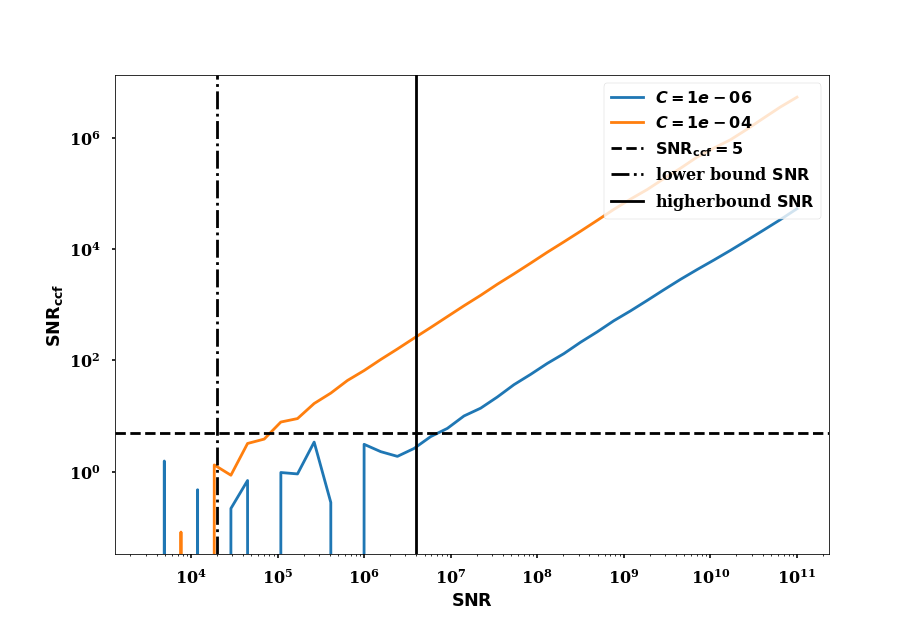
\includegraphics[scale =0.5]{images/Chapter3/parspace_new.png}
    \caption{Caption}
    \label{fig:parspace-1}
\end{figure}
On the x-axis is $\rm{SNR}$ and on the y-axis is the $\rm{SNR_{ccf}}$. 
The horizontal dashed line represents the cut off of $\rm{SNR_{ccf}}>6$ which is our cut off.
The orange and blue lines represent those spectra with exoplanets at a contrasts of $10^{-4}$ and $10^{-6}$.
The two vertical lines consist of the upper and lower bound of the $\rm{SNR}$. 
The window between the two vertical lines consists now of spectra where very few exoplanets with a contrast of $10^{-6}$.
An interesting observation is that beyond an $\rm{SNR}>5$ the relationship between $\rm{SNR_{ccf}}$ and $\rm{SNR}$ becomes linear and thus it validates our cut off criterion.

\paragraph{Parameter space selection of $R$:\\}
The parameter space of $R$ is limited by the resolution of the \textsc{BT-SETTL} library itself and hence we limit ourselves to a $R<300,000$. 
We choose a sampling rate of $50$ between $10^{2}$ and $10^{5}$ so that we have a total of $20$ different resolutions for each spectrum.

\subsection{The detection matrix }
The goal of defining the parameter space and designing the algorithm was to populate the detection and characterization matrices.
Given the context here, the detection matrix itself is not very difficult to explain and is indeed somewhat self explanatory. 
However, it is important to still define what each row and column means in the detection matrix for warm Jupiters in Fig~\ref{fig:detmat}
\begin{figure}[!ht]
    \centering
    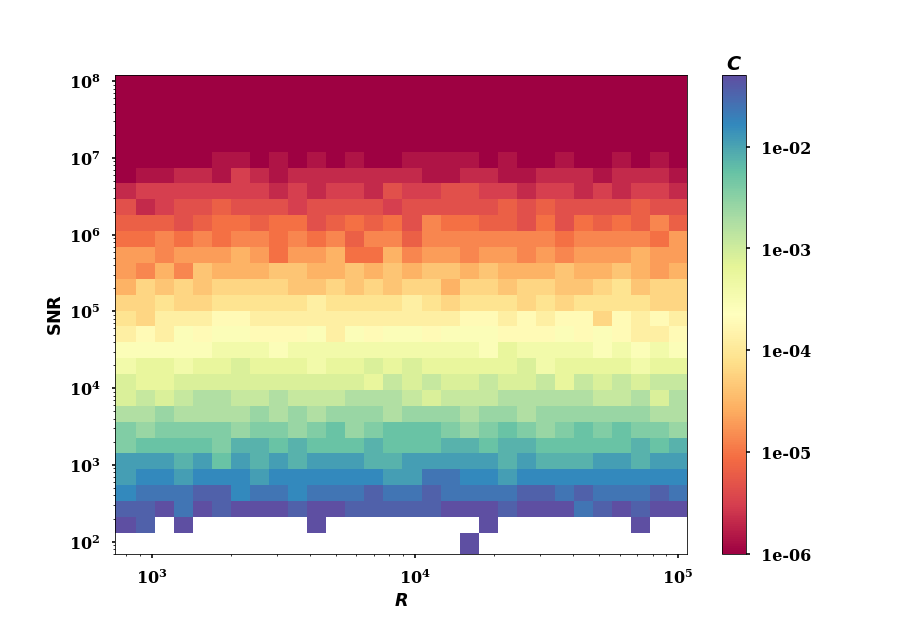
\includegraphics[scale=0.5]{images/Chapter3/detmat.png}
    \caption{Caption}
    \label{fig:detmat}
\end{figure}
This detection is produced as described in the methods chapter.
Each cell in the matrix represents a contrast between $10^{-1}$ and $10^{-6}$.
From the bottom to the top the rows represent $\rm{SNR}$ values from the lowest to the highest.
The bottom two rows i.e $\rm{SNR}<300$ contain a lot of white cells, these are cells where even for the unphysically low contrasts of $0.1$ the exoplanets were not detected. 
These $\rm{SNR}$ represent cases where no matter what the $R$ and $C$ are the exoplanet is completely undetectable.
There are many interesting points to note from this detection matrix.
As with Fig~\ref{fig:parspace-1} we saw that a linear relationship exists between the $\rm{SNR_{ccf}}$ and $\rm{SNR}$ which implied that the $\rm{SNR}$ seems to directly influence the cross correlation strength.
The detection matrix seems to reinforce this idea when detecting faint exoplanets.
As the $\rm{SNR}$ increases the matrix gets redder indicating the detectability of fainter companions. 
The top $3$ rows are at a detection limit of $10^{-6}$, this means that the faintest companion is completely detectable for the highest signal to noise of the spectrum.

Another interesting point to be noted in this matrix is when the $\rm{SNR}$ is fixed for higher $R$ there is no measurable improvement in sensitivity of detection of faint exoplanets.
There are a some slight improvements in detection sensitvity at higher $\rm{SNR}$ particularly at $\rm{SNR}\approx 10^{5}$ and $R\approx 5\times10^4$ where we are able to detect a slightly higher contrast exoplanet.
But once we increase the $\rm{SNR}$ we wash out any differences there may be at higher resolution.
Note that for a constant $\rm{SNR}$ as $R$ increases $\rm{SNR_{\lambda}}$ reduces, therefore the advantage of having several wavelength bands is outweighed by lower $\rm{SNR_{\lambda}}$.
Using this detection matrix, it is clear that for warm Jupiters, this trade-off indeed means that increase of $R$ no discernable advantage for detection.
\subsection{Characterization error bars }
\label{sec:char error bars}
The characterization of an exoplanet consists of two subsequent steps,
\begin{enumerate}
    \item produce the characterization matrix with either the $\rm{SNR_{ccf}}$ or $LL$ where both the matrices have to be mirror images of each other and
    \item fit the inverse Gaussian to $LL$ characterization matrix.
\end{enumerate}
For the first part, it is important to first look at a sample plots of the characterization matrices at specific values from the parameter space.
We choose a spectrum with a $T_{\rm{eff}}= 1500$ and a $\rm{\log(g)} = 4.5$.
We start with a lower $\rm{SNR}$ where the exoplanet is not detectable in Fig~\ref{fig:nondet_char}.
\begin{figure}[!h]
    \centering
    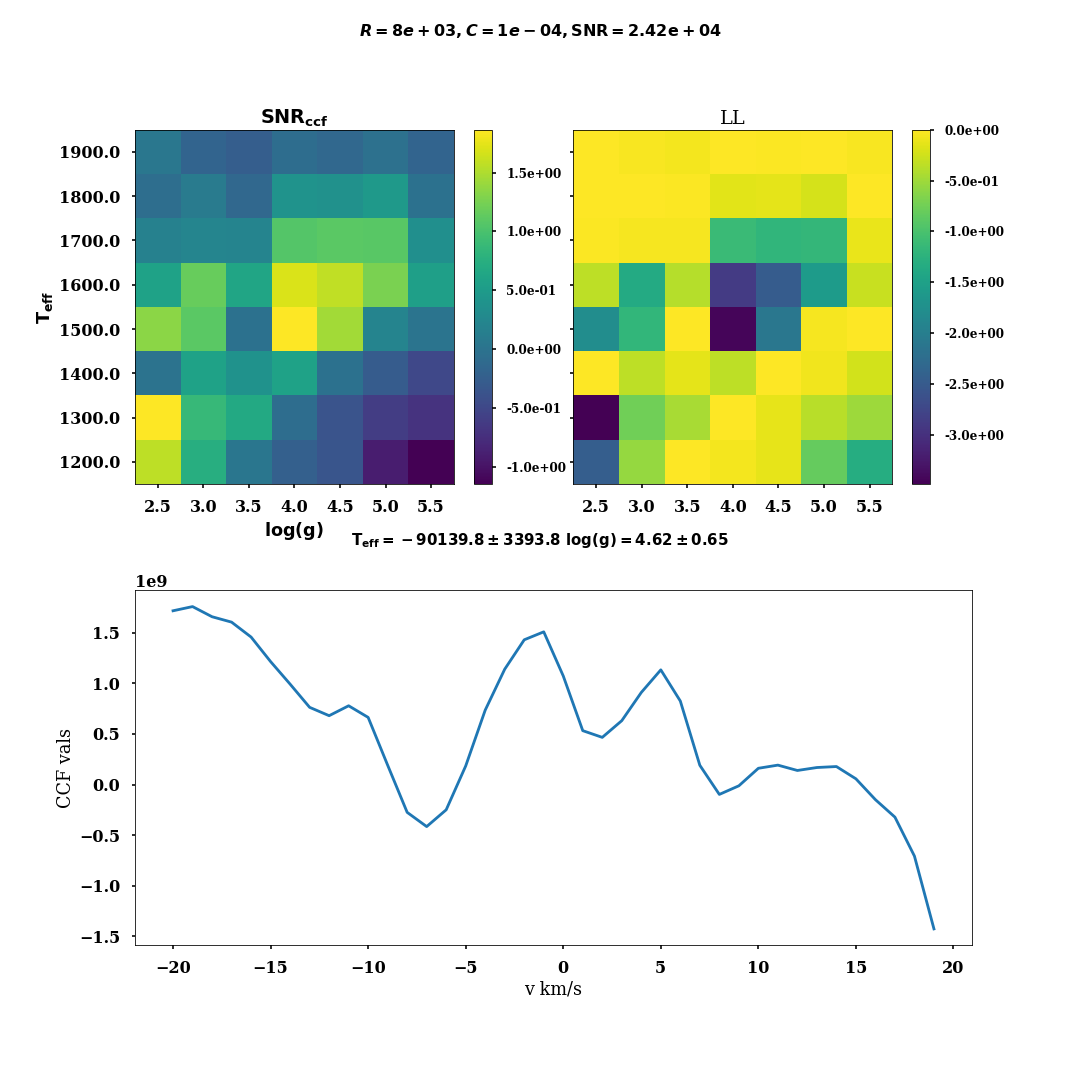
\includegraphics[scale=0.4]{images/Chapter3/char_plots_8e+03_1e-04_2.42e+04.png}
    \caption{Caption}
    \label{fig:nondet_char}
\end{figure}
The top left is the characterization matrix with $\rm{SNR_{ccf}}$ as the parameter within the matrix and $LL$ as the parameter on the top right.
The bottom of the plot is the shape of the cross correlation function with respect to the velocity.
Note that for the contrast involved this exoplanet is not detectable and appropriately it is not possible to quantify the error bar in the effective temperature.
This also reinforces the idea of having a characterization hypothesis where the exoplanet is characterizable only if an exoplanet is definitely detectable.
Based on Fig~\ref{fig:detmat} as we increase the $\rm{SNR}$ we will be able to detect the exoplanet. 
At $\rm{SNR_{ccf}}<5$ the relationship is still not linear and therefore, it is possible that we don't have enough photons in enough wavelength bins to have a detection and characterization. 
Therefore, we depict a case where $\rm{SNR_{ccf}}>5$ inf Fig~\ref{fig:charmap-det}
\begin{figure}[!h]
    \centering
    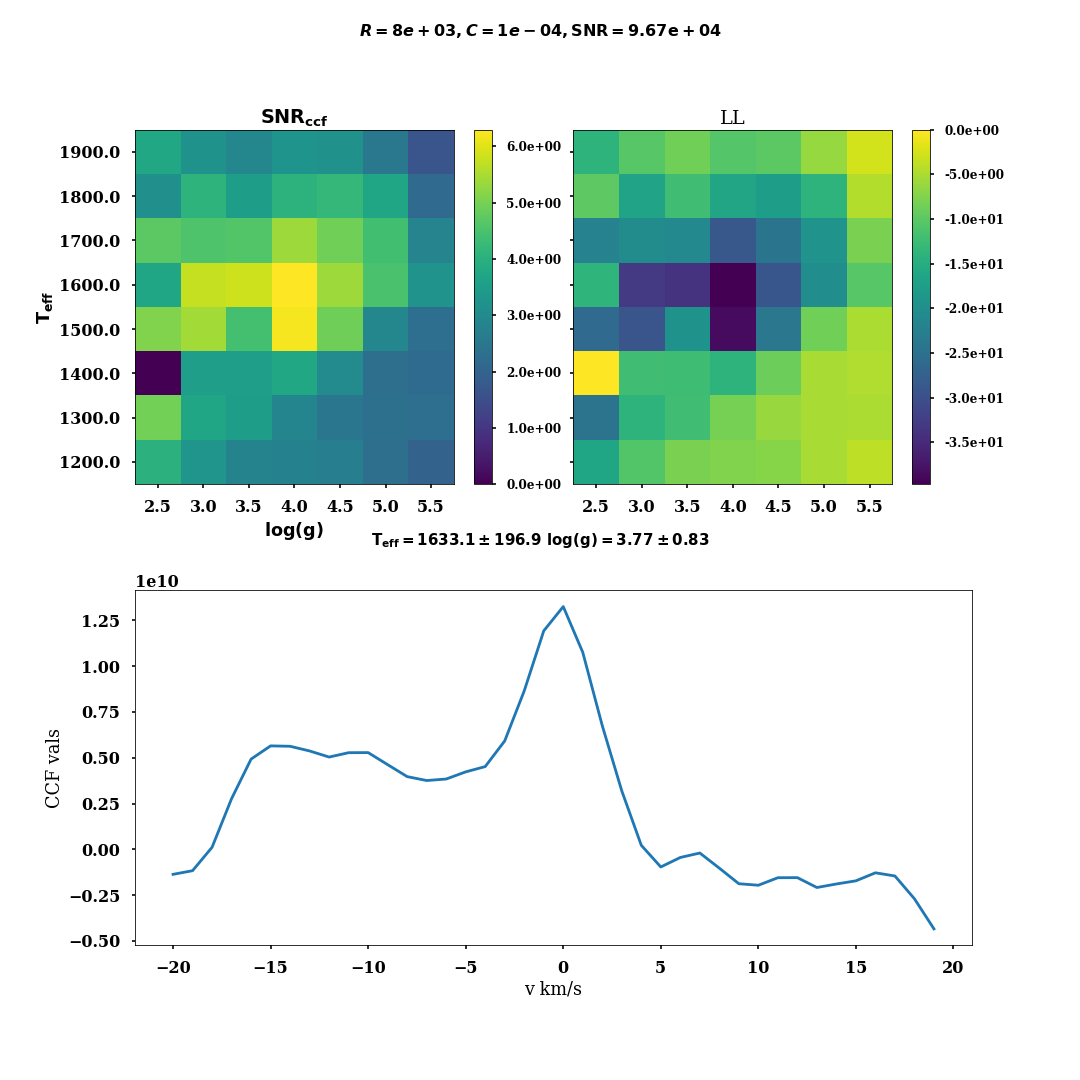
\includegraphics[scale=0.4]{images/Chapter3/char_plots_8e+03_1e-04_9.67e+04.png}
    \caption{Caption}
    \label{fig:charmap-det}
\end{figure}
A couple of interesting points of comparison between these two last figures,
\begin{enumerate}
    \item Firstly, when $\rm{SNR_{ccf}}<5$ we notice that the depth of the $LL$ is fairly shallow. 
    This results in a wild estimate of $\rm{T_{eff}}$ whereas a more reasonable estimate of $\log(\rm{g})$ is present but this is because of the limited number of bins.
    \item Secondly, the shape of the cross correlation over velocities is strikingly different, which is also reflected in the depth of the $LL$.
    This also brings to light the close relationship between detection and characterization.
    In fact the shape of the cross correlation along velocity seems to indicate the accuracy of fit in the characterization matrix.
    \item Finally, the relevant question that is raised when both the plots are compared is whether, increasing the $\rm{SNR}$ even further will result in a more accurate estimate of $\rm{T_{eff}}$.
    If that is not the case, then could increasing the resolution lead to better constraints on the effective temperatures and surface gravities?
\end{enumerate}
We answer the first question by cross correlating a spectrum with a much higher $\rm{SNR}$.
Fig~\ref{fig:charmap-deeptrough} shows a case where the cross correlation values are much higher and the distribution of the cross correlation over velocities is much more Gaussian like.
This also leads a 'deeper' trough in the $LL$.
\begin{figure}[!ht]
    \centering
    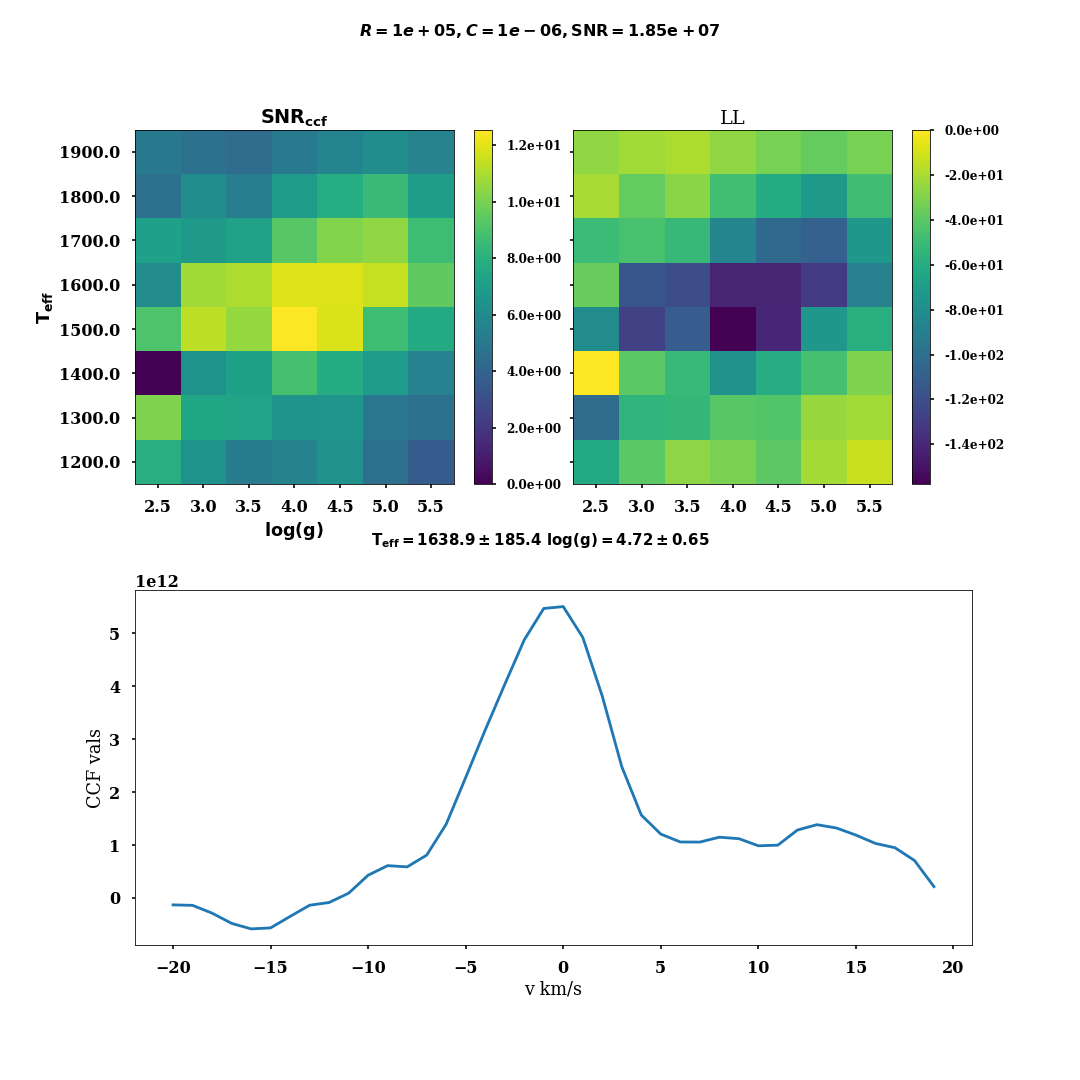
\includegraphics[scale=0.3]{images/Chapter3/char_plots_1e+05_1e-06_1.85e+07.png}
    \caption{Caption}
    \label{fig:charmap-deeptrough}
\end{figure}
However, this does not produce a narrower trough because of the velocity resolution. 
Consequently, the characterization accuracy does not improve. 
While the $\log(\rm{g})$ is slight above one template resolution unit ($0.5$ dex) the $\rm{T_{eff}}$ has an error bar $\approx 200$K which is twice the resolution unit of $100$K. 
This error bar also is quite close to the error bar at $\rm{SNR}$ where the exoplanet is just detected.
This shows that increasing $\rm{SNR}$ does not produce a more accurate characterization, whereas for detection a higher $\rm{SNR}$ does produce fainter detections.

Finally, to answer the question of whether increasing the resolution will change this behaviour, we produce the same plot for a higher $R$ with similar $\rm{SNR}_{\lambda}$.
Note that we lower the $C$ so that it still continues to be comparable in terms of $\rm{SNR_{ccf}}$ in Fig~\ref{fig:highres-charmat}.
\begin{figure}[!ht]
    \centering
    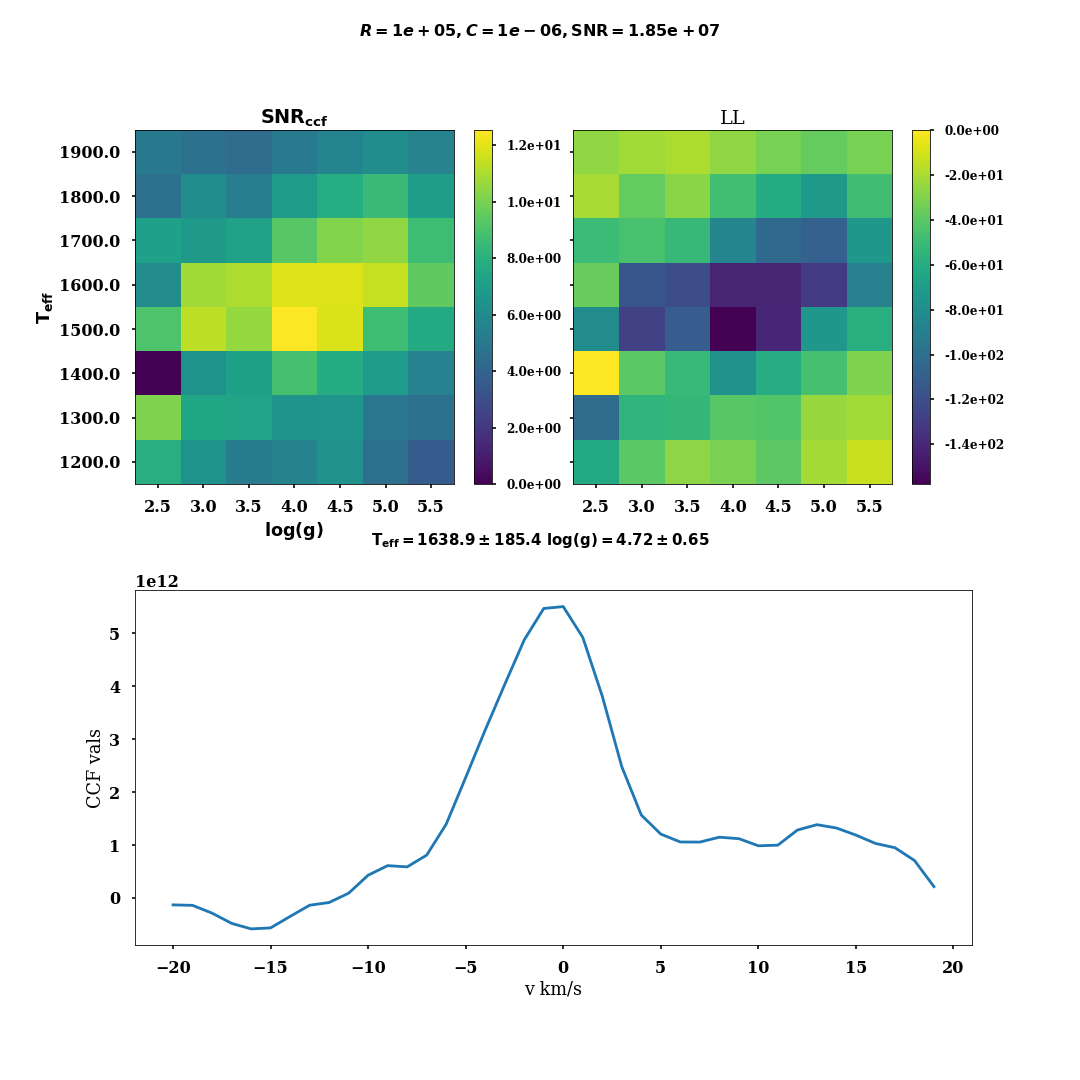
\includegraphics[scale=0.3]{images/Chapter3/char_plots_1e+05_1e-06_1.85e+07.png}
    \caption{Caption}
    \label{fig:highres-charmat}
\end{figure}
It is, thus, clear that there is a theoretical limit to how accurate a characterization can be.
This is not influenced by any parameters beyond the fact that the exoplanet is detectable in the spectrum.
It is also interesting, that the width of the Gaussian of the cross correlation does not get narrower and consequently it appears that the width of the $LL$ is also equally wide.
This width as we have seen defines the $\sigma_x$ which is our error bar.
In the discussion section of this chapter we will define the benchmark that the cross correlation algorithm sets for the ML algorithms and what steps the ML algorithms need to pass to be considered usable for scientific analysis.

\section{Benchmark for ML algorithms}
In lieu of having a discussion section, we will discuss the results that were produced using the cross correlation algorithm and its consequences for the detection and characterization hypotheses.
Given these consequences, we will then define what the benchmark for the ML algorithms are. 
Finally, we will discuss how these consequences could help the scientific community.
\subsection{The detection hypothesis and the relevant benchmark}
The detection hypothesis states that given the appropriate spectral parameters, it is possible to detect an exoplanet with unlimited sensitivity.
We define sensitivity as the ability to detect faint exoplanets while having $<10^{-4}$ average false positive rate.
We then composed a detection matrix to quantify this sensitivity as a function of the observation parameter $\rm{SNR}$ and the instrumental parameter $R$.
Within this detection matrix we filled the contrast at which the exoplanet was detectable in the spectrum for an $\rm{SNR_{ccf}}\ge6$ for a defined $\rm{SNR}$ and $R$.
We found that $R$ had very little effect on the sensitivity of detection, but beyond a $\rm{SNR}>10^{5}$ the exoplanet at the lowest contrast was detectable at all values of $R$. 
This result has some interesting consequences firstly for the next step whereby it will set the benchmark for the ML algorithms and secondly for the scientific goals of using exoplanet spectra in general.

\paragraph{Setting the benchmark for ML algorithms:\\}
The question that this part of my thesis seeks to answer is whether ML algorithms, with their ability to learn patterns, can learn a generalized pattern corresponding the features of exoplanet spectrum to identify those spectra which contain them.
We define this problem to be complicated by three broad parameters, $C,R \& \rm{SNR}$.
The detection matrix allows us to establish where in the parameter space are traditional algorithms most sensitive to the exoplanet. 
We have now established that to have the highest sensitivity, the cross correlation algorithm requires a minimum $\rm{SNR} =10^{5}$.
This then implies that there definitely is enough planetary features which could be matched with a template.
The detection matrix also justifies that $R$ has very minimal to no impact on  detection sensitivity.
Therefore, the first benchmark goal for ML algorithms would be two fold,
\begin{enumerate}
    \item within the parameter space that the cross correlation detection algorithm achieves its highest sensitivity, the ML algorithm also needs to perform as well and this will be quantified using confusion matrices to begin with and 
    \item if ML algorithms achieve a mean false positive rate $<10^{-4}$ and true positive rate $>0.5$ in this parameter space, they will be used to construct a similar detection matrix.
\end{enumerate}
This step would validate that ML algorithms are indeed a reasonable replacement for the cross correlation algorithm. This means that ML algorithms through this methodology can be used to estimate the sensitivity of datasets.
Finally, for ML algorithms to be considered better than cross correlation based algorithms it needs to satisfy the following conditions, in addition to the above,
\begin{enumerate}
    \item they need to be more sensitive to fainter companions, with the same false positive rate, at lower $\rm{SNR}$ and
    \item to be just as flexible with increasing $R$ with the same sensitivity.
\end{enumerate}
\paragraph{Consequence for the scientific goals of spectral data processing to detect exoplanets:\\}
The detection matrix allows us to estimate the parameter space that is ideal for detection sensitivity to be maximized.
It also allows us insight into certain parameters that limit the detection sensitivity.
One of the key goals of scientific data collection and processing is to identify the values within parameter space that allows us to achieve the scientific goals.
The detection matrix aims to be the basis to establish these values for specific scientific cases.
The scientific case that we make at this point is the detectability of warm Jupiters using spectra at different $\rm{SNR}$ and $R$.
More specifically, we aim to define at what contrasts are these warm Jupiters detectable.
In the case of warm Jupiters, it is clear the $\rm{SNR}$ is the most important parameter that limits the sensitivity of detection.
An interesting observation is that this sensitivity does not change with increasing $R$ where the $\rm{SNR_{\lambda}}$ decreases for a fixed $\rm{SNR}$.
The detection sensitivity is thus directly related to the overall $\rm{SNR}$ than to the $\rm{SNR}_\lambda$ for each wavelength bin.
Therefore, using this matrix it is clear that for $\rm{SNR}=10^{4}- 10^{5}$, which is the mean $\rm{SNR}$ that is achieved for an observation such as \textcolor{blue}{[Refer to observations in Part II HD142527b]} we will be able to detect a warm Jupiter at a $C\approx 10^{-4}$.

Another interesting consequence, is the rate at which sensitivity improves in the detection matrix.
In Fig~\ref{fig:parspace-1} it was clear that there is a linear relationship between the $\rm{SNR}$ and $\rm{SNR_{ccf}}$ particularly beyond $\rm{SNR_{ccf}}\ge 5$.
This means that beyond this value an increase in $\rm{SNR}$ produces a an increase on $\rm{SNR_{ccf}}$ in the detection matrix as it is composed of only contrasts where the $\rm{SNR}_{ccf}>6$.
Thus for an increase in $\rm{SNR}$ we should logically see a uniform increase in the detected $C$. However, what we observe is that this increase is not uniform, whereas it increases quite rapidly for lower contrasts $C<10^{-4}$ but increases much slower for higher contrasts.
This is a very interesting behaviour which seems to indicate that for this sort of data detections beyond $10^{-4}$ may be difficult to pass.
We will see this progress in more detail in \textcolor{blue}{[Refer Part II Chapter results]}.

Finally, we see that for increase in $R$ there is little to no impact on detection. 
This is particularly interesting, because we would expect that for a constant $\rm{SNR}$ an increase in $R$ will produce a drop in $\rm{SNR_{\lambda}}$. 
This means each of the wavlength bins have fewer signal photons and therefore the cross correlation strength should reach $\rm{SNR}_{ccf}=6$ only when more overall photons are available (i.e at higher $\rm{SNR}$. 
But it appears that overall $\rm{SNR}$ (which is constant along a row) is the only aspect that influences detection and not $\rm{SNR_{\lambda}}$.
We posit that this is the case because of the large number of wavelength bins available, the mean $\rm{SNR}$ is a bigger factor than individual photons in individual bins.
Thus the advantage of higher resolution can be seen for this problem with not losing sensitivity to detection.
This might have been a very good case for higher resoluion instruments if the characterization showed improved results with resolution.
\subsection{The characterization and its relevant benchmark}
\label{sec:removal of stellar}
Characterization, in this thesis, is defined as being able to constrain the $\rm{T_{eff}}$ and $\log(\rm{g})$ of an exoplanet with consistent error bars.
Our characterization hypothesis states that we should be able to characterize any spectrum where an exoplanet exists.
The word exists is precisely quantified by the detection algorithm as having a $\rm{SNR_{ccf}}\ge 5$.
This is evidenced when we use the characterization matrix on spectra at fixed $R,C$ and varying $\rm{SNR}$.
We notice that the $\rm{T_{eff}}$ constraints become consistent after after an $\rm{SNR_{ccf}}\approx 3.5$.
It is, therefore, clear that the quantification of the characterization parameters are heavily influenced by the ability to detect exoplanet spectra. 

We designed a characterization matrix with two things in mind,
\begin{enumerate}
\item to constrain the mean $\rm{T_{eff}}$ and $\rm{\log(g)}$ of a spectrum with an exoplanet along with the independent uncertainties of both these quantities and also,
\item to ensure that we are able to do this for all spectra where a exoplanet spectrum can be detected.
\end{enumerate}
The goal of this matrix is not to quantify the evolution of the error bars or the mean of the $\rm{T_{eff}}$ and $\rm{\log(g)}$ with spectral parameters such as $\rm{SNR}$ and $R$ unlike the detection matrix.
However there are still some interesting points to note and these points will define the characterization goals for ML algorithms.
This involves three broad ideas,
\begin{enumerate}
    \item the evolution of the characterization accuracy,
    \item the impact of the stellar subtraction on characterization accuracy and
    \item the intimate relationship between detection and characterization.
\end{enumerate}
\paragraph{Evolution of the characterization accuracy with the parameter space:\\}
When comparing the error bars over a parameter space we will use the detection matrix in Fig~\ref{fig:detmat} for two purposes,
\begin{enumerate}
    \item to make the link between \textit{detectability} and accurate characterization of the exoplanet spectrum
    \item and secondly to demonstrate the handy of the detection matrix when describing the evolution of science goals (in this case detection and characterization) with the parameter space.
\end{enumerate}
When we look at the evolution of both $\mu_x$ and $\sigma_x$ in the characterization matrix in Fig~\ref{fig:nondet_char} to Fig~\ref{fig:charmap-det} the first point is the evolution of the $\mu_x$ i.e the mean $\rm{T_{eff}}$ and $\rm{\log(g)}$ does not got any closer to the template $\rm{T_{eff}}=1500$K as we move along the rows in the detection matrix.
This property is also true for the $\log(g)$. 
This is a marked diversion from the behaviour of the cross correlation algorithm when used as a detector.
While moving along rows we detect fainter exoplanets, it does not seem to translate that this implies the template is closer (i.e accurate mean) to the one that was inserted.
As we move further along the rows and we increase the $\rm{SNR}$ to more than double, we still see little to no effect on the detection accuracy and it appears that even now there is no way to have a perfect characterization.
This once again marks a departure with detectability where as we move to unphysically high $\rm{SNR}$ values in the top rows we get an almost uniformly perfect sensitivity to detection.

Following this line of thought, the evolution in the $\sigma_{\rm{T_{eff}}}$ and $\sigma_{\rm{\log(g)}}$ is also unsurprising.
However, what is surprising is the fact that error bars remain for as large as two grid points for the $\rm{T_{efF}}$ and slightly more than one grid point for $\log(g)$.
The question, therefore, is what is producing this large error bar. 
The fact that even with higher $R$ this problem is not alleviated shows that intrinsically there is an uncertainty produced by a single quantity left untouched so far i.e $C$.
When we reproduce the same plots for $C=10^{-1}$ which is not only physical but does not have any other detection analog, we see that we get near perfect characterization.
\begin{figure}[!ht]
    \centering
    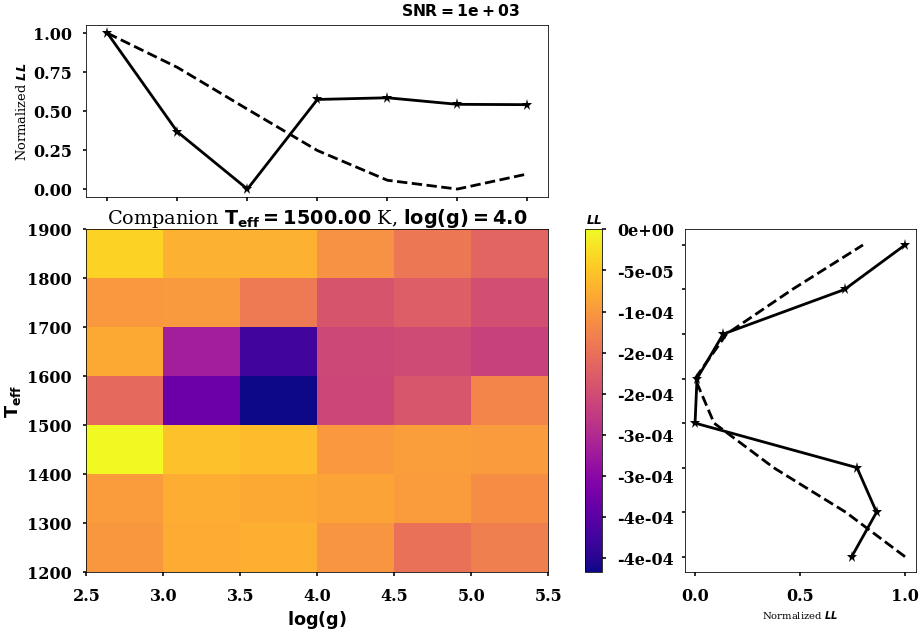
\includegraphics[scale=0.5]{images/Chapter3/char_fits_0.png}
    \caption{Caption}
    \label{fig:perfectchar}
\end{figure}
An example is shown if Fig~\ref{fig:perfectchar}.
We also show the fits to convince ourselves that indeed this fit is an inverse Gaussian fit and the contrast is the parameter the produces a more accurate $\mu_{\rm{T_{eff}}}$.
But even though the mean $\rm{T_{eff}}$ is accurately retrieved there is a fairly large error in the $\log(\rm{g})$ characterization.
But from this map it is fairly clear what the reason for the inaccurate $\rm{T_{eff}}$ characterization is.
If indeed the characterization accuracy and thereby its error bars are constrained by the presence of stellar contaminants, would there be a better accuracy when the star is switched off?
\textcolor{red}{Talk about the ML characterization goal}
\paragraph{Effect of perfect removal of stellar signal from the data:\\}
While this thesis relies on limited pre-processing and is indeed tuned to removing any stellar features from the data, no pre-processing is perfect and leaves some residual stellar contamination in the data.
An easy way to test this is to `switch off' the star and this is fairly easy to do with synthetic data by setting $C=1$ in Eq~\ref{eq:insertion}.
This would be the case where the stellar signal is perfectly subtracted. 
Note that the data still contains observation noise and contains the intrinsic randomness of that noise.
We computed different characterization matrices for such spectra for different $\rm{SNR}$ and $R$ (note that $C=1$ is now a constant).
\begin{figure}[!ht]
    \centering
    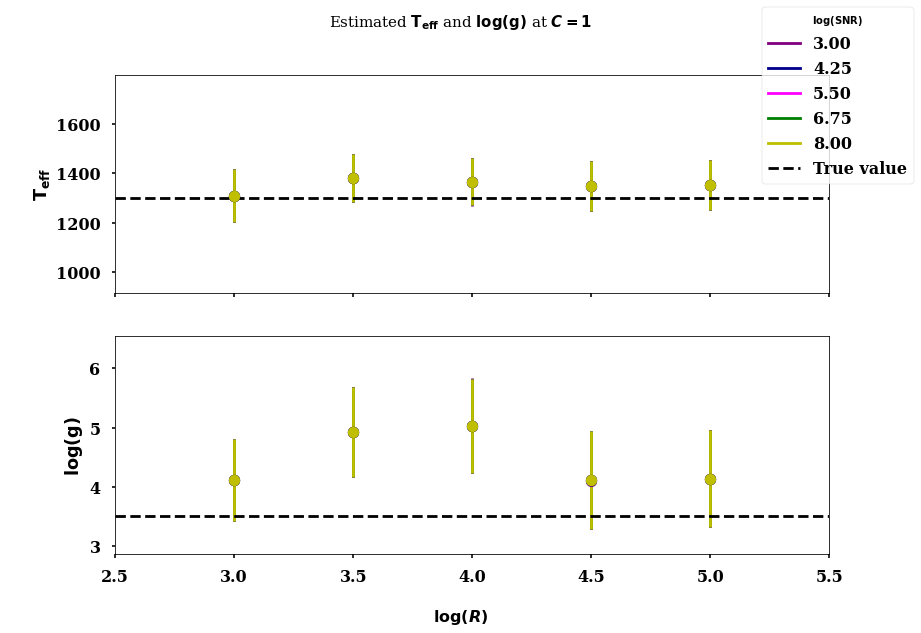
\includegraphics[scale=0.5]{images/Chapter3/char_teff_logg_C1.png}
    \caption{Caption}
    \label{fig:ceq1}
\end{figure}
Fig~\ref{fig:ceq1} shows the evolution of the estimated $\mu_{\rm{T_{eff}}}$ and $\rm{\log(g)}$ for different values of $\rm{SNR}$ and $R$.
This is a very interesting plot as the legend seems to indicate that there are different $\rm{SNR}$ values but the plot just shows one color. 
The reason for this is that the different $\rm{SNR}$ values perefectly overlap with no difference in $\rm{T_{eff}}$ and $\log{(\rm{g})}$ estimation.
The dotted line indicates the original $\rm{T_{eff}}$ and $\rm{\log(g)}$ of the exoplanet.
There are at least two interesting takeaways from this plot,
\begin{enumerate}
    \item unlike the detection matrix, the effect of $\rm{SNR}$ is absent but the contrast and perfect stellar subtraction is the biggest reason for inaccurate characterization.
    This is quite interesting because the cross correlation based detection seems to behave as a signal processing problem where with higher $\rm{SNR}$ we have perfect detection.
    However, the characterization of an exoplanet seens to behave as an astronomical processing problem whereby we need perfect stellar subtraction to achieve perfect characterization.
    \item Secondly, we notice that while the $\rm{T_{eff}}$ is perfectly characterized and indeed is defined by a nice $LL$ curve, the $\log(\rm{g})$ is not so well characterized. 
    In fact when we see the evolution of characterization accuracy we see the effect of increasing $R$ upto an $R=10^{4}$ after which this effect is take over by the presence of more absorption lines.
\end{enumerate}
The second point is fairly well defined in that based on Eq~\ref{eq:line} the $\rm{SNR_{\lambda}}$ will decrease with increasing $R$ for a fixed $\rm{SNR}$ and therefore when $\rm{SNR_{\lambda}}$ is the defining parameter to achieve a scientific goal we will see this mitigated with increasing $R$.
Characterization seems like one such goal where the best characterization seems to occur at low $R$ and high $R$ and in between we see a loss of characterization accuracy.
This particularly more evident in the case of $\log(\rm{g})$ where we work with a smaller baseline and therefore fitting a $LL$ curve is not that straightforward.

This leads us to the limitations of this method and how we expect the ML algorithms to perform better than this.
The primary limitation is the need to have a more accurate characterization method whereby the characterization matrix can be populated accurately over a larger range of contrasts.
The error bar on this characterization matrix needs to be stable over multiple $\rm{SNR}$.
However, as we have seen with the cross correlation algorithm, this is not an easy task with spectra.
Therefore,the first benchmark for ML algorithms is to identify the region in parameter space of $R,\rm{SNR}$ where we are able to characterize an exoplanet spectrum with the lowest error for $C<10^{-2}$.
This can the be followed by higher contrast characterizations if it is successful.
Note that this is subject to the condition that ML algorithms are able to make high contrast detections, i.e they are able to learn the spectral features of exoplanets at various contrasts.

\paragraph{Link between detection and characterization of spectra:\\}
An outcome of the characterization has been that in many ways the characterization accuracy is unrelated to the detection sensitivity.
However, both detection and characterization are being performed with the same spectra and the same algorithm that relies on the same spectral features.
Therefore, the question that remains to be explored is whether there is indeed any link between the two operations and if so why does this link disappear so that characterization accuracy does not improve in a lockstep manner with detection sensitivity.

Firstly the link between detection and characterization is most evident when we look at Fig~\ref{fig:nondet_char} and the equivalent detection sensitivity in Fig~\ref{fig:detmat}.
It is clear that when the cross correlation algorithm is not able to detect the exoplanet with the related $C$, the characterization accuracy is very low.
To produce the detection matrix we need to have the following relationship satisfied
\begin{equation}
    \dfrac{\rm{CC(0)}}{\sigma}\ge6
\end{equation}
allowing that the $\rm{AC}$ is mostly a constant value and the variation is the $\sigma$ and the $CC(0)$.
At $CC(0)$ there is no relative wavelength shift between the spectrum and the template.
Therefore based on \textcolor{blue}{[refer to Eq from Part II]}, we can rewrite it as ,
\begin{equation}
    CC = \sum\limits_{\lambda} F_{\rm{\lambda_{1},noisy}}M_{\lambda_1}+ F_{\rm{\lambda_{2},noisy}}M_{\lambda_2}+\cdots+F_{\rm{\lambda_{N-1},noisy}}M_{\lambda_{\rm{N-1}}}+F_{\rm{\lambda_{N},noisy}}M_{\lambda_{\rm{N}}}
    \label{eq:CC(0)expansion}
\end{equation}
and therefore we can now re-express the condition with the simplification that $\sigma = \rm{SNR}$ as 
\begin{equation}
    \dfrac{\sum\limits_{\lambda} F_{\rm{\lambda_{1},noisy}}M_{\lambda_1}+ F_{\rm{\lambda_{2},noisy}}M_{\lambda_2}+\cdots+F_{\rm{\lambda_{N-1},noisy}}M_{\lambda_{\rm{N-1}}}+F_{\rm{\lambda_{N},noisy}}M_{\lambda_{\rm{N}}}}{\rm{SNR}}\ge 6
\end{equation}
Thus, for a single entry in the detection matrix the sum of the products of the template and the spectrum has to be $\ge 6\times \rm{SNR}$.
Thus the sum of products in Eq~\ref{eq:CC(0)expansion} can be expressed as a limit of the $\rm{SNR}$ which explains why for increase in $\rm{SNR}$ we see an increase in detection sensitivity.
Thus detection sensitivity can be re-interpreted as the minimum value of the product in Eq~\ref{eq:CC(0)expansion} for which the sum of the photon values in each bin with the template is high enough to be detected.
Thus it serves as a mimimum criterion for characterization and hence for values where $\rm{SNR}<5$ the characterization accuracy will provide very unstable errorbars.
This is then the fundamental link between detection and characterization.
However, why is there not an unlimited improvement to characterization accuracy to reach perfect characterization?

In order to achieve perfect characterization we see that we need to have $C\approx1$.
In such a case we will re-write Eq~\ref{eq: true signal} as,
\begin{equation}
    F_{\rm{total},\lambda} = F_{\rm{planet},\lambda}
\end{equation}
and thus the the noisy spectrum is re-written as,
\begin{equation}
    F_{\rm{noisy},\lambda} = \textrm{random}(\textrm{PMF}(F_{\rm{planet},\lambda}))
\end{equation}
which means the noisy spectrum does not contain random values from the stellar spectrum.
Therefore, when $LL$ is calculated there needs to be higher specificity to template features to produce a deep $LL$ trough. 
This is provided only when $C\to1$ than to $C\ll 1$ which is the case for higher contrast. 
Hence, the characterization accuracy is no longer dependent on $\rm{SNR}$ but on the intrinsic exoplanetary signal present in the spectrum which is described by $C$ rather than $\rm{SNR}$.
Naturally, the characterization accuracy would not boundlessly increase as the $C$ is bound for a portion of the detection matrix.
On the other hand when we de-link it from the detection matrix we find that we are able to achieve perfect characterization.
Thus the detection and characterization are only related until the point when the characterization itself is possible but not to increase the characterization accuracy which is independent of detection.

\subsection{Why would ML algorithms be an asset if they work?}
The goals for the ML algorithms is thus two fold,
\begin{enumerate}
    \item define the limits at which ML algorithms are able to detect warm Jupiters in either context of the detection matrix or om a part of the detecton matrix parameter space and
    \item define the characterization accuracy for this part of the of the detection matrix generated by the ML algorithms.
\end{enumerate}
Before we explain why this thesis posits ML algorithms to be an asset should they work, we need to explain the reasons to test ML algorithms in the context of this chapter.
Firstly, the cross correlation algorithm as is defined in this section is limited to processing the data with one sample spectrum at a time.
The results however, have to be analyzed for more than one spectrum at a time, for instance we take $10$ noise realizations for each cell of the detection matrix and almost $50$ different templates have to be cross correlated to produce one characterization matrix is produced.
This is a perfect case for batch processing, but also statistical variations between spectra needs to be handled better than by mere averaging.
Secondly, there is no unified model for warm Jupiters that is discerned with the use of cross correlation, each template spectrum is treated as a unique spectrum whereas in reality the variation between spectra is not so unique as typified in the characterization matrix in Fig~\ref{fig:charmap-deeptrough} where $\rm{SNR_{ccf,\mu}}$ is still $>3$. 
This implies that when sufficient photons exist, all the templates provide enough similarity with test spectrum to produce a detetion.
Finally, this algorithm is still limited by the interpretation of the cross correlations through a $\rm{SNR_{ccf}}$ or $LL$ which have their own set of biases and therefore, provide only a analysis bias limited result.

This then provides the framework for ML algorithms to be, if successful, a nice alternative to the cross correlation based algorithm.
Firstly, ML algorithms are able to analyze batches of spectra and provide batch outputs and thus can populate the detection matrix much faster and with a generalized manner.
The need to train ML algorithms is a feature which allows us to train the algorithms with physical parameters that are varied.
This in turn will produce an ML algorithm that has learned the `physics' of the spectrum than working purely from the signal processing stand point.
We expect that this is more useful for astronomers, than to fine tune the cross correlation algorithms from a signal processing standpoint.
Secondly, the fact that the biases of ML algorithms are well quantifiable, by means of receiver operating characteristic curves for example, means that the algorithmic biases can be well understood. 
The statistical fluctuations can also be well quantified  with the help of a large and varied dataset.
This means we don't rely only on averaging the results but will be able to limit these statistical fluctuations by controlling the variance in the data.
Finally, the use of ML algorithms will constitute a fast, robust and reliable way to detect and characterize the spectrum simultaneously and we will use the parameter space from the chapter to train the ML algorithms on.
\chapter{Development and performance of the ML algorithms}
\label{chap:III.5}
In the previous chapter we presented the cross correlation based detection and characterization algorithms along with the results for a clearly defined parameter space.
For the training, validation and testing of ML algorithms in this chapter we continue use the same data set as in the previous chapter.
The advantage of being able to generate a practically unlimited number of spectra allows us to extend our scope to try to cover as much of the top five rows of the detecton matrix as possible.
We confine ourselves to using the highest $\rm{SNR}$ cases for two reasons,
\begin{enumerate}
    \item the top rows allows us a a full range of contrasts to test if the faintest exoplanet detected by the cross correlation algorithm is still reachable by the ML algorithms
    \item and to ensure that the lack of photons does not limit our ability to test ML algorithms in the field of high contrast exoplanet detection.
    This would serve as the best opportunity to test the ability of ML algorithms with a large observing baseline.
\end{enumerate}
The results of that chapter will serve as the basis to develop the ML algorithms used in this chapter.
In this chapter, we describe the ML algorithms that are used for this part in my thesis. 
The goals of this chapter are the following,
\begin{enumerate}
    \item describe the parameter space and the motivation for the use of parameter space based on the results of the previous chapter. This will form the "data" description in this chapter.
    \item Describe the motivation and development of the ML algorithms that will be used in this part of the thesis. The background description of these algorithms are assumed from §\ref{chap:III.2}. 
    \item Describe first the results of the cross correlation algorithm evaluation using the confusion matrices described in §\ref{chap:III.3} followed by the algorithm evaluations of the ML algorithms used.
    \item Finally, we end this chapter with a discussion on why the ML algorithms were not used in further science evaluations and its consequences for the use of spectra with ML algorithms.
\end{enumerate}
\begin{comment}
Describe how these case studies were chosen and why they are relevant to the study.
What do we learn when they fail or pass
In order for ML to be considered \textit{more effective} it needs to be able to make detections at higher contrast than $(C\approx10^{-2}$ for a $\rm{SNR}\le10^4)$ across $R$.
\end{comment}
\section{Experimental parameter space selection and testing they hypotheses}
The parameter space begins with identifying the combination of $(R,\rm{SNR},C$ for the purposes of training, validation and testing the ML algorithms.
The goal of this exercise is to primarily divide the parameter space into two broad categories,
\begin{enumerate}
    \item identify cases that would serve as the basis to evaluate the ML algorithms and "fail fast" if the algorithms need to be marked as not appropriate for this purpose. 
    A failure to make the appropriate false positive bar would lead the algorithms trained to be marked as inappropriate for this problem. 
    A pass at this stage using confusion matrices indicates that ML algorithms are eligible to check for higher contrast cases which will allow us to compose the detection matrix.
    \item The second category would be the highe contrast cases where the contrast is high enough that only higher $\rm{SNR}>10^{4}$ will be able to detect the exoplanets in these spectra.
    This second category is the tipping point to define if ML algorithms can indeed be compared with the cross correlation algorithm.
\end{enumerate}
In this section we will begin with describing the problem statement that will be used with ML algorithms first for detection and then for characterization.
The hypotheses statements still remain valid and therefore they have to be tested with ML algorithms.
We will follow this with describing the parameter space that will be chosen for each category and both the scientific and data challenge posted by this parameter space.
\subsection{Adapting ML algorithms to test the detection hypothesis}
In order to test the detection hypothesis, the first step is to pose the problem accurately so that an ML algorithm can be used to test the hypothesis.
The detection hypothesis was tested using the cross correlation algorithm by inferring the conditions (namely $R$ and $\rm{SNR}$) that are necessary to achieve perfect detection (namely detecting an exoplanet at $C=10^{-6}$).
The condition for detection was set at $\rm{SNR_{ccf}}\ge 6$ due to its low false positive rate,
The $\rm{SNR_{ccf}}$ is defined as the single parameter that will allow us to determine the fitness of the exoplanet to be detected.
Thus, we have shown that with the detection hypothesis can be proven with the use of the a detection criterion parameter ($\rm{SNR_{ccf}}$), the detection criterion ($\rm{SNR_{ccf}}\ge 6$) and the detection matrix.
The detection parameter will continue to remain the contrast at which we meet the detection criterion when applied to the detection criterion parameter.
Following this recipe, we will also define the first two criteria for ML algorithms when validating the detection hypothesis. 
The detection matrix remains the same to be used for both the ML algorithms and the cross correlation algorithm.

\paragraph{Detection criterion parameter:\\}
The ML algorithms are able to provide two types of outputs as discussed in \Cref{chap:III.2} namely categorical or a regression output.
We explained that when the classes of the output are well known the categorical or classification problem is best chosen.
In this case we can have two possibilities for each spectrum, either it contains features for an exoplanet or it does not contain these features. 
These categories are of course not well separated because a high contrast exoplanet may not be detectable at all.
This was the reason for the detection hypothesis, which states that there are indeed conditions where the exoplanet is detectable with an appropriate algorithm.
We used the detection matrix to find the conditions where the parameter space separates the spectra as having exoplanet features and therefore detectable even at the highest contrast and not having exoplanet features and therefore not detectable.
We use this idea to define the problem of ML algorithms as a classification problem. 
Given the right conditions the spectra should be clearly separable as containing an exoplanet or not containing one.
The detection criterion parameter, therefore is a class of whether an exoplanet exist $y=1$ or not $y=0$ and therefore we re-express Eq~\ref{eq: true signal} and Eq~\ref{eq:insertion} as 
\begin{eqnarray}
    C_y =& y\times C\\
    F_{\rm{planet},\lambda,new} =& C_y\times F_{\rm{planet},\lambda,old}\times \rm{SNR}^2\\
    F_{\rm{total},\lambda} =& (1-C_y)F_{\rm{star},\lambda,new} + F_{\rm{planet},\lambda,new}
    \label{eq:ML_detect_eqn}
\end{eqnarray}
The rest of the equations continue as before from §\Cref{chap:III.3}.
We are thus able to generate spectra to be used as training for ML algorithms.
As with any classification algorithm, the value of $y$ is universally only $0$ or $1$ but lies on a sigmoid curve such that when the exoplanet features exist $y\to 1$ and when they don't exist $y\to0$.
Therefore, a second criterion to the detection criterion parameter is necessary such that we can quantize $y$.We choose the criterion as $y =1$ when $y>0.5$ and $y=0$ when $y\le 0.5$.

In order to understand how the spectral features of the noisy spectrum in \Cref{eq:insertion} evolves with different contrasts we present a series of plots where the contrast is reduced and this produces a higher $\rm{SNR_{ccf}}$.
Note that the $\rm{SNR_{ccf}}$ is sensitive to changing $C$ exponentially, whereas it is related to $\rm{SNR}$ linearly.
\Cref{fig:compare-specsnr=5.24} shows a spectrum generated with a $\rm{SNR}$ with two classes, $y=0$ in pink and $y=1$ in green. 
The topmost plot is a sample template spectrum re-sampled to the spectral resolution $R=1000$.
The bottom most plot shows the cross correlation strengths as a function of velocity of both the pink and the green spectra.
Note that visually, it is not possible to tell apart the green and pink spectra, but the cross correlation algorithm is able to make this distinction.
In order to also illustrate a case where the difference between the pink and green spectra is stark, we choose a very high $\rm{SNR}$ and low $C$ in \Cref{fig:compare-specsnr=3000}.
We can clearly see the shape of the template and its specific features in the K-band and H-band.
\begin{figure}[ht]
    \centering
    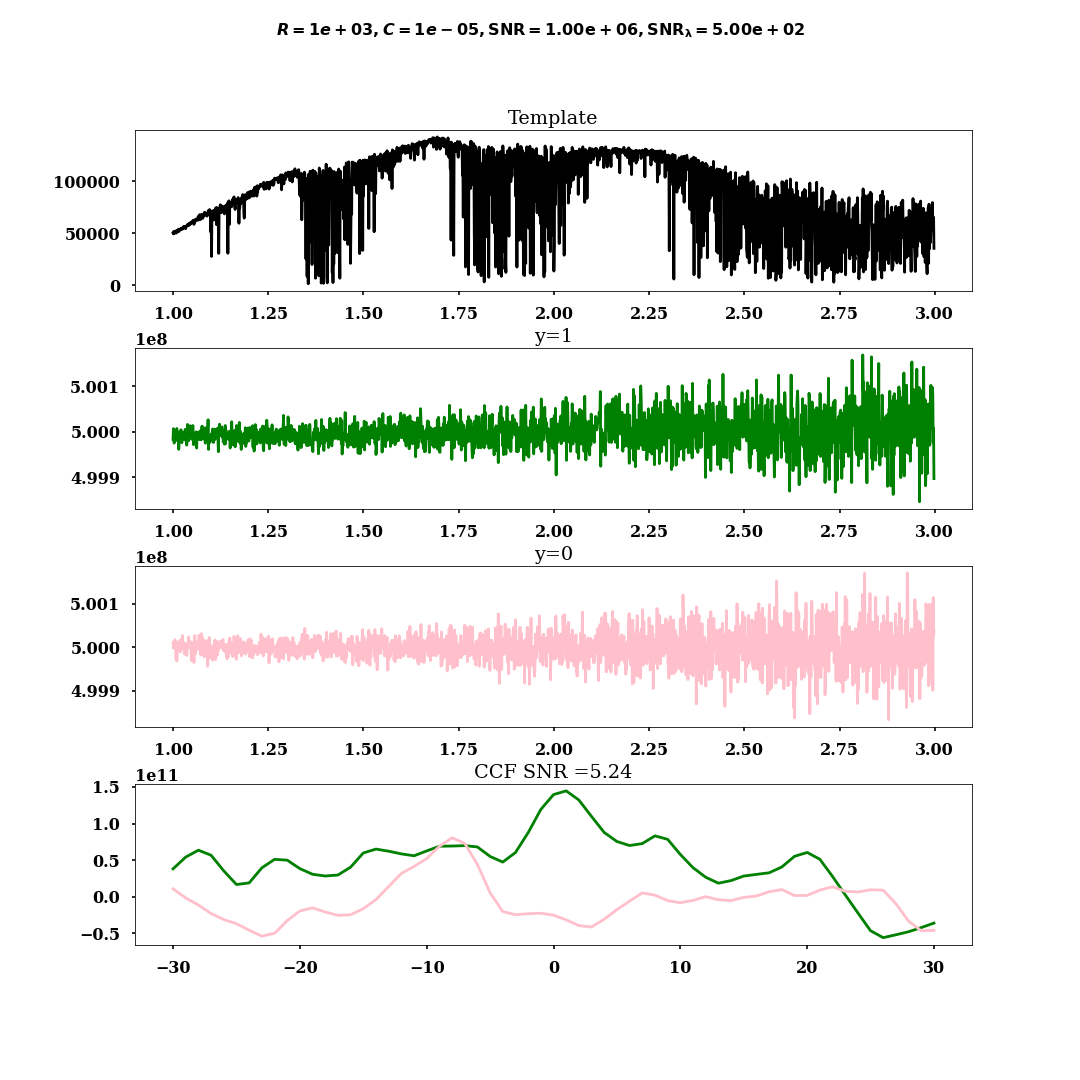
\includegraphics[width=\textwidth]{images/Chapter3/feature_compare_ccf_snr_5.24.png}
    \caption{Caption}
    \label{fig:compare-specsnr=5.24}
\end{figure}

\begin{figure}[!hb]
    \centering
    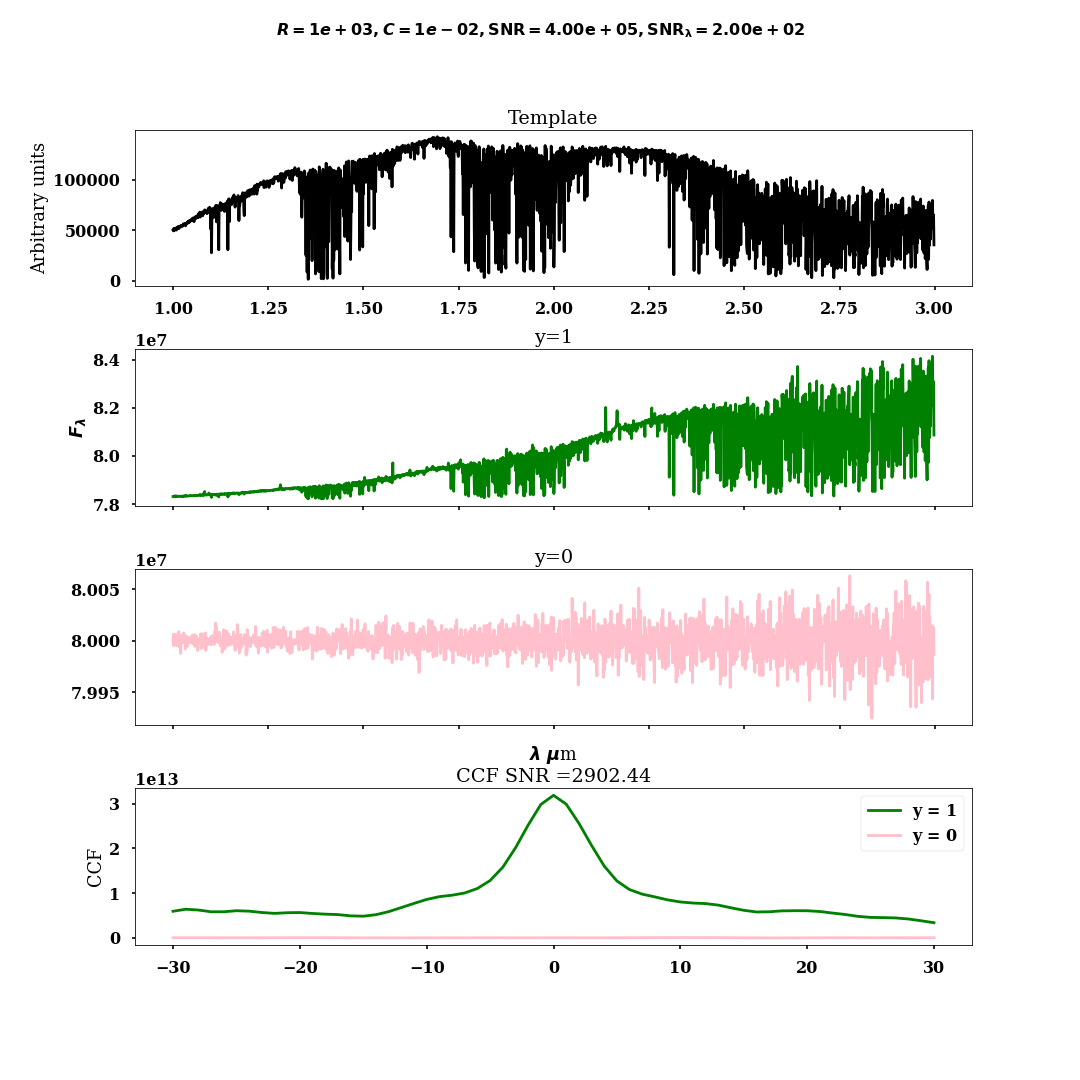
\includegraphics[width =\textwidth]{images/Chapter3/feature_compare_ccf_snr_2902.44.png}
    \caption{Caption}
    \label{fig:compare-specsnr=3000}
\end{figure}
Thus, we have the detection criterion parameter $y$ that will serve as the prediction parameter for the ML algorithms with the spectra being inputs.
\paragraph{The detection criterion:\\}
The final part of adapting ML algorithms is to establish the detection criterion that needs to be met in order to test the detection hypothesis.
As stated above when the output of the ML algorithm is between $0.5$ and $1$, we quantize the output to mean the predicted value of $y$ ($y_{\rm{pred}}$) which will then be used to populate the detection matrix.
The detection matrix as constructed using the cross correlation algorithm was built by simultaneously analyzing a large number of spectra and then populating the matrix with the results of this analysis.
For ML algorithms, as explained in \Cref{chap:III.2}, we need to train, validate and test these algorithms taking care to not overfit the data.
A lot of the overfitting will be taken care by providing sufficient variance in the data described in \Cref{subsec:paramspace}.
For the purposes of describing generating the detection matrix, it is sufficient to say that we generate over $15000$ spectra in total to produce the training, validation and test datasets.
The detection criterion still remains the detectable contrast $C$ and we will establish the mean contrast that is detectable for a range of $\rm{SNR}$ and $R$, once again chosen with a criterion similar to \Cref{fig:parspace-1}.

In order to now establish the detection criterion for a specific parameter values we proceed with the following steps,
\begin{enumerate}
    \item we first generate a large number of spectra with one specific template with variations being made in $\rm{SNR}$ and $C$ but a fixed $R=1000$. We divide these spectra into training, validation and test datasets.
    We then train the ML algorithms with the training  datasets and use the validation dataset to fine tune the following parameters, the learning rate gradient, the momentum, the mix of contrasts involved and the hyper parameters of the ML algorithm being used.
    The first two are changed continuously during training depending on validation error, but the mix of contrasts is changed so that the validation error is $\approx 10^{-5}$.
    We then test the algorithms with the test data by producing confusion matrices.
    \item When the false positive rate is low enough, we proceed to generate fresh spectra in the contrast ranges used for training (no matter the validation error) and compute the confusion matrices for these. 
    These will be exactly the same as the test confusion matrices but to rule any statistical uncertainties we produce fresh spectra.
    We use these confusion matrices and identify the highest contrast where we can produce a confusion matrix so that the true positive rate $>0.5$ and the false positives produces are $1$ for $10000$ spectra.
    \item We then perform this operation for each of the $\rm{SNR}$ in the parameter space and identify $C$ to populate the detection matrix.
\end{enumerate}
Note that we will start with highest $\rm{SNR}$ to ensure that we rule out the possibility of that ML algorithms fail the detection hypothesis.
\subsection{Adapting ML algorithms to test the characterization hypothesis}
The characterization hypothesis is tested using the characterization matrix.
As with detection matrix, the characterization matrix is populated by the characterization parameter which was the $LL$ in \Cref{chap:III.4}.
The characterization parameter could have also been $\rm{SNR_{ccf}}$, but for reasons explained in \Cref{chap:III.4} we use $LL$ which is the negative square of the $\rm{SNR_{ccf}}$.
We don't have any known literature which connects the value of $y_{\rm{pred}}$ and any Gaussian distributed parameter that will allow us to derive a $\chi^{2}$ error bar.
Therefore, in this subsection we will briefly describe two different strategies to produce a characterization parameter and the merits and demerits of both. 
It is to be noted that if the ML algorithms fail the detection hypothesis, there is not enough evidence that they will be able to test the characterization hypothesis.

As already explained in \Cref{sec:classifcation and regression}, supervised algorithms are either classification or regression algorithms. 
In practice this means that either the output of the ML algorithm is completely unbounded or is bounded to remain between $0$ and $1$.
Since we don't have any prior art in this regard, we postulate using both regression and classification as approaches to produce the characterization matrix.
The caveat of this section is that neither of these approaches were validated as ML algorithms failed the detection hypothesis, but this section is evidence of clear experimental planning before we explain the ML algorithms.
\paragraph{Use of regression to compute the characterization parameter:\\}
When using regression to compute the characterization parameter, we directly compute the $\rm{T_{eff}}$ and $\rm{\log(g)}$ from the ML algorithms.
The question is how doe we compute the error bars on these quantities.
We first define the output of the ML algorithm to be two quantities i.e $\rm{T_{eff}}$ and $\rm{\log(g)}$ for each spectrum.
We then use an appropriate error function such as the mean square error to compute the error on these quantities.
As the mean square error will be the quantity minimized, we will have the minimum mean square error on these quantities separately.
However, in order to compute the true error bar we had posited the following steps,
\begin{enumerate}
    \item generate a large number of spectra for a fixed value of $\left(C,R, \rm{SNR}\right)$ so that each spectrum represents only a different noise realization. Based on our results in \Cref{sec:char error bars} and \Cref{sec:removal of stellar}, it is clear that the biggest effect on characterization error bars is the stellar contamination. 
    \item fit a non-parametric curve to the results produced from these spectra to compute the means and standard deviations.
    \item this will result in one mean and standard deviation for both $\rm{T_{eff}}$ and $\rm{\log(g)}$ for each combination of $(C,R,\rm{SNR})$ and
    \item finally, we will generate characterization matrices for each value of $C,R$ for several $\rm{SNR}$ to produce a result akin to \Cref{fig:perfectchar}.
\end{enumerate}
This can then be used to verify that the error bars are quantifiable for specific values of $C$.
The advantage of this technique is that we can directly regress to the value of $\rm{T_{eff}}$ and $\rm{\log(g)}$.
The disadvantage of this method is that it is possible the distribution of $T_{eff}$ and $\rm{\log(g)}$ does not lend to accurate error or mean calcuation, in which case it would be pointless. 
This type of regression does not lend to clean graphical qualification of the performance of different templates.
Hence we will also explore a slightly different way of quantifying the mean and standard deviation
\paragraph{Design of a characterization matrix with a logistic characterization parameter:\\}
The goal of the characterization matrix is to compute the mean $\rm{T_{eff}}$ and $\rm{\log(g)}$ and their uncertainties.
We also like a nice graphical way that can describe the similarities between different templates.
To achieve this we define a new parameter $p$ such that,
\begin{equation}
    y_{\rm{pred}} = p
    \label{eq:p-ypred}
\end{equation}
The distribution of $p$ for a single spectrum is \Cref{fig:sample charmat}.
\begin{figure}
    \centering
    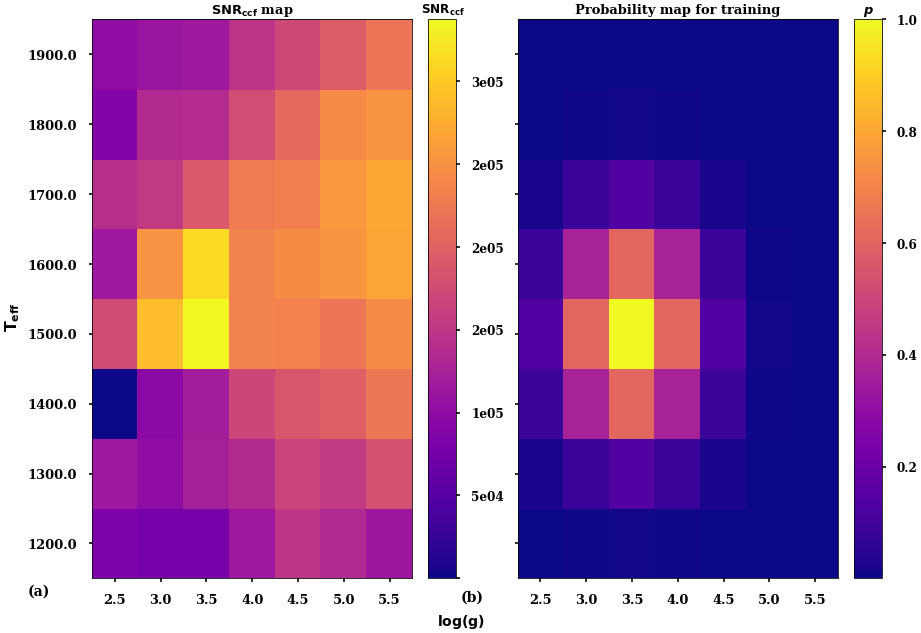
\includegraphics[width=\textwidth]{images/Chapter3/subplots_snr_p.png}
    \caption{Caption}
    \label{fig:sample charmat}
\end{figure}
For every spectrum, we will have a characterization matrix with different $p$ values.
The $p$ values are distributed as a 2D Gaussian centered on the $\rm{T_{eff}}$ and $\rm{\log(g)}$ of the template of the exoplanet.
A sample map is shown in \Cref{fig:sample charmat} alongside a characterization map with $\rm{SNR_{ccf}}$ as the characterization parameter.

We posit that a ML algorithm can learn to recognize feature strengths that vary as a Gaussian centered around the inserted template.
The standard deviation of this Gaussian will give us uncertainties of both $\rm{T_{eff}}$ and $\rm{\log(g)}$.
We will use a logistic error function such as the categorical cross entropy to minimize the training error.
We will generate large number of spectra with constant $\rm{SNR},R$ and slightly varying $C$ so that we can have some variance in the data.
We will automatically produce these characterization matrices and train the ML algorithms to produce the same matrices for every spectrum.
The advantage of this approach is that we get a characterization matrix which has a parameter that can be related to detection.
We can also get a very good visual reference for large number of spectra and verify that the error bar is consistent for different types of spectra.
Finally, these matrices allow us to infer whether ML algorithms are able to distinguish between templates in one glance.
The disadvantage of this approach is that there is no evidence that the output of ML algorithms will obey this distribution.
There is also little evidence to show that \Cref{eq:p-ypred} holds true for large number of spectra with any bounding condition.

\subsection{Parameter space selection}
\label{subsec:paramspace}
The parameter space selection is simplified by the tests performed using the cross correlation algorithm and the resulting detection and characterization matrices.
There are two takeaways from these tests that we will continue to work with while choosing the parameter space to train, validate and test the ML algorithms,
\begin{itemize}
    \item the $\rm{SNR}$ is the most important parameter to validate the detection hypothesis, in turn this means that for the highest $\rm{SNR}$ the detection hypothesis has the highest chance of being validated for all contrasts concerned.
    Note that this does not preclude that ML algorithms will automatically perform exactly as the cross correlation algorithm has performed, but merely chooses the best possible chance for ML algorithms to succeed.
    \item Secondly, it is clear that detection and characterization are linked through the contrast, where we know that if the contrasts are low and $\rm{SNR}$ we are able to perform simultaneous detection and characterization. But what needs to be seen if ML algorithms are able to consistently find the spectral features for different contrasts to convince us to use them to characterize spectra.
\end{itemize}
Point 2 thus raises an important question, i.e will ML algorithms work on both the low and the high contrast space.
With this in mind, while keeping $10^{5}>\rm{SNR}>10^{6}$, we divide our parameter space into a low contrast parameter space corresponding to $C>10^{-3}$ and a high contrast parameter space $10^{-3}>C>10^{-4}$.
\paragraph{Low contrast parameter space:\\}
The low contrast parameter space is defined where the contrast is between $10^{-2}>C>10^{-1}$.
As described earlier, we choose the highest $\rm{SNR}$ between $10^{5}>\rm{SNR}>10^{6}$ to give the ML algorithms the best chance to train.
We fix the $R=1000$ for two reasons, firstly that there has not been significant evidence to show that $R$ has much impact on the detection or characterization of an exoplanet particularly when testing our hypotheses.
Secondly, higher $R$ means higher number of bins and consequently larger memory and computational requirements.
Therefore, we choose a low $R$ to test our hypotheses with ML algorithms.
As stated before, we generate a large number of spectra based on \Cref{eq:ML_detect_eqn}.
In order to keep this fair we also validate the spectra by running them through the cross correlation algorithm and setting a $\rm{SNR_{ccf}}>5$ to set the $y_{\rm{pred,ccf}}$.
We sample the parameter space such that the distribution of spectra is fully within the sample space.
To illustrate this we plot the spectra generated based on the parameter space, such that a single spectrum generated with a combination of $\rm{SNR},C$ is represented as a single point in \Cref{fig:trained_sample space}.
The sample space is filled with three colors pink points corresponding to $y=0$, black corresponding to spectra undetected by the cross correlation algorithm ($y=1$) and green points corresponding to those that are detected. 
The absence of black points in \Cref{fig:trained_sample space} shows that there are no spectra which are missed by the cross correlation algorithm.
This plot also illustrates that the parameter space is well filled and the balance between $y=0$ and $y=1$ spectra is fairly even.
\begin{figure}[!h]
    \centering
    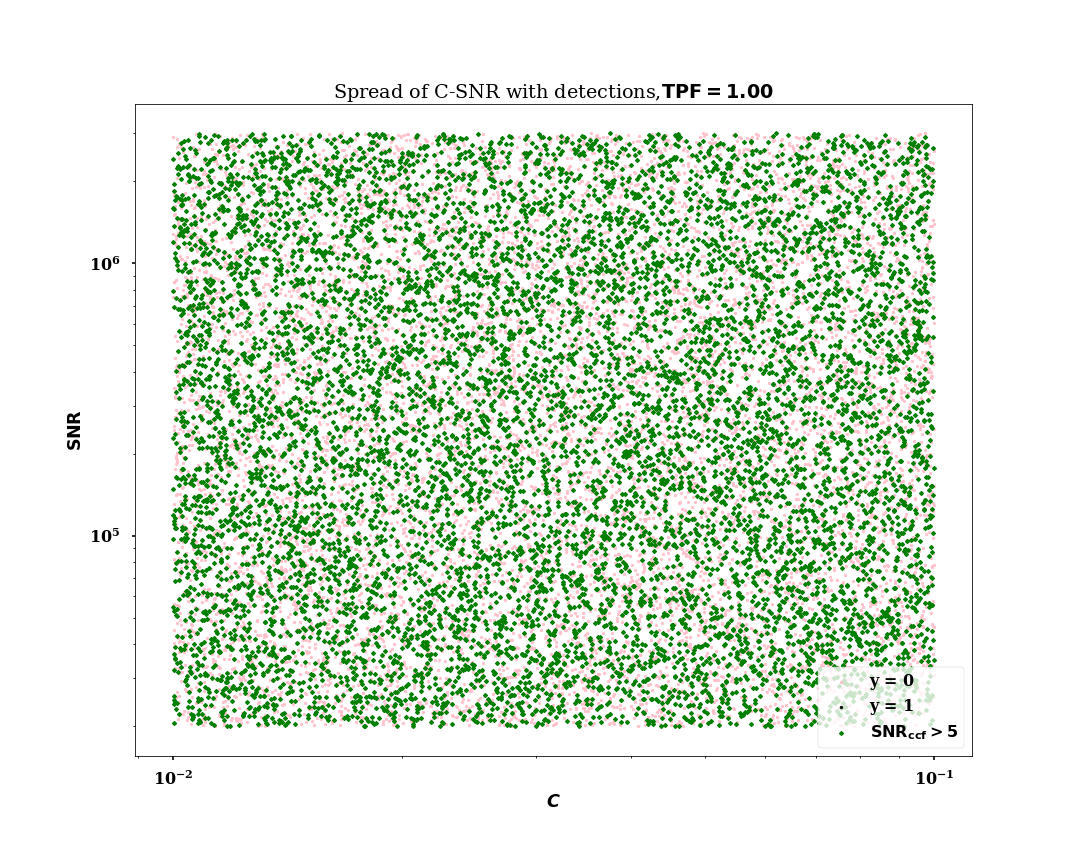
\includegraphics[scale=0.4]{images/Chapter3/samples_trained.png}
    \caption{Caption}
    \label{fig:trained_sample space}
\end{figure}
\paragraph{high contrast parameter space:\\}
For the high contrast parameter space we choose a contrast range of $10^{5}>C>10^{3}$. 
In principle we could choose the highest contrast, but we also wanted make a parameter space where the true positive rate for the cross correlation algorithm was slightly higher than $0.5$.
This gives us confidence that majority of the spectra indeed contain features that are detectable by a `classical' algorithm. 
At the same time there are a few samples that provide a `challenge' to the ML algorithms to detect.
A similar plot to \Cref{fig:trained_sample space} is used to depict the samples drawn from this parameter space.
In \Cref{fig:untrained_sample space} we see some black dots filling up $\approx 30\%$ of the parameter space, whereas the rest of the parameter space is covered by green dots.
Note that $\rm{SNR_{ccf}}>5$ is a somewhat `high bar' to ensure we don't end up with a high false positive rate and does not mean that those spectra which deliver a $\rm{SNR_{ccf}}\approx 4.5$ are non detectable or that they don't contain features that are detectable.
\begin{figure}
    \centering
    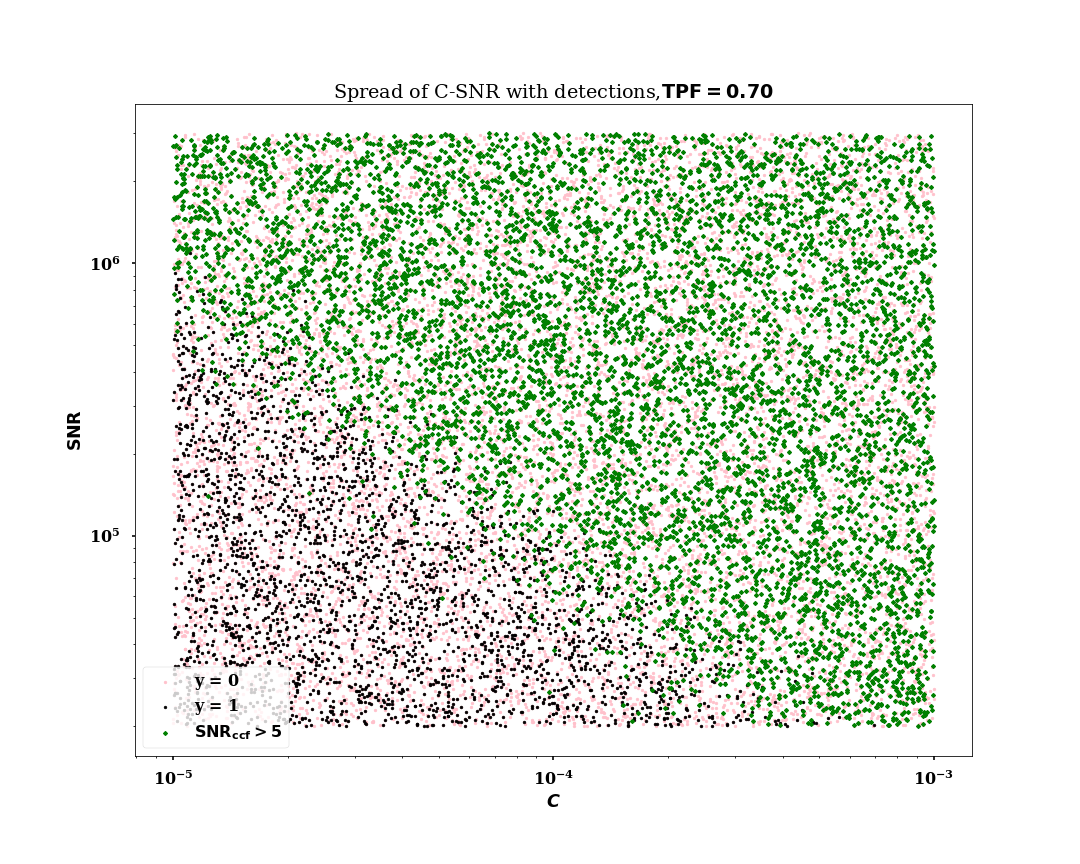
\includegraphics[scale=0.4]{images/Chapter3/samples_nontrained.png}
    \caption{Caption}
    \label{fig:untrained_sample space}
\end{figure}

When reporting the results we will make this discrimination of high and low contrast parameter spaces as the results also are neatly divided in between these parameter spaces.
A final word on this parameter space is that while the contrast cut off between the spaces is somewhat arbitrary, there is a clear scientific justification for dividing these contrasts.
Firstly, the low contrast cases are what would be really bright targets and therefore, if known they would correspond to the first set of targets that would be used to test new instruments and algorithms.
These would also correspond to targets whose properties of $\rm{T_{eff}}$ and $\rm{\log(g)}$ are well defined and so they can be well quantified and verified.
In principle, therefore this parameter space represents some of the well defined targets.
Secondly, the high contrast space is that which is typical of targets that are the most numerous in the high contrast imaging.
Therefore, this represents the targets that ML algorithms will most likely be presented with and therefore the performance on this parameter space is the test of failure of ML algorithms. 
It is on this parameter that we need to quantify the performance of ML algorithms on.
\section{ML based algorithms}
ML algorithms come in different flavours and types and a brief introduction to this was presented in \Cref{chap:III.2}.
As stated earlier, this thesis primarily works with supervised classifiers to test the detection hypothesis and we could choose supervised classifiers or regressors to test the characterization hypothesis.
As we shall see in the  \Cref{sec:ML results} the performance of ML algorithms did not provide us with the confidence to try out characterization strategies.
Therefore, this section will primarily discuss the algorithms used for testing the detection hypothesis.
However, we would be remiss in assuming that these algorithms could not be adapted to test the characterization hypothesis.
We will, therefore, also suggest ways to adapt this algorithm for the characterization case.
We will discuss later the ways that spectra could be used directly with ML algorithms that is out of the scope of this thesis but could be tried out easily in the future with the framework provided by this thesis.

\textcolor{red}{This is a very crucial paragraph which justifies how what I have done different from 2020 Fisher.
Note there are indeed very many similarities and it is possible this is one of the weakest points, that it is not fair to expect any characterization from ML as the Fisher paper exactly reports this.
I aim to justify this as 1. I use detection to test if this method can be used with HCI data 2. we then will move to characterization iff we are able to compose the detection matrix with ML algorithms.}
As described in \Cref{chap:III.2}, supervised classifier algorithms come in different types, in this thesis we use ensemble and deep learning algorithms.
The goal of trying two different kinds of algorithms is to verify whether a) are results consistent over different types of algorithms and b) whether any kind of algorithm offers an advantage to this type of analysis.
As stated before \cite{2020Fisher} has explored the use of random forests and deep learning algorithms with cross correlation data, which are similar in the sense that they are also large 1D vectors.
However, the same algorithms have not worked with spectra directly, when ML algorithms have been used to constrain the metallicity and temperature directly from the spectra.
There are two fundamental differences from how we are posing the problem,
\begin{enumerate}
    \item firstly, we pose this problem as a pure detection problem where we are detecting an exoplanet as an inference based on the presence of an ensemble of exoplanet features in the spectra and
    \item secondly, the characterization part of the problem is essentially an extension of the detection where we identify the closest template to the one that is present in the data and use that to infer the properties of the exoplanet.
    \end{enumerate}
    In addition we choose the parameter space of the spectra after carefully whetting it by running them through the cross correlation algorithm. Finally, we will use the ML algorithms to first the detection hypothesis to define if ML algorithms are able to validate it before validating the characterization hypothesis.
Our ML detection and characterization algorithm is a three step algorithm,
\begin{enumerate}
    \item in the first step we conduct the data generation and normalization where we generate the data specified by the parameters of $C,R,\rm{SNR}$ this is followed by,
    \item the passing of the spectra through the ML algorithms which either detect or could produce a characterization output and finally,
    \item this is terminated with a analysis step which is usually either a confusion matrix where we know the truth values or a threshold application.
\end{enumerate}
The final step is the scientific outcome that is relevant to this thesis.
\subsection{Data generation and pre-processing}
We first generate data as in \Cref{fig:trained_sample space} for the low contrast parameter space.
We choose a range of templates to initially begin with in order to minimize the chance that the ML algorithm will memorize wavelength features specific to the template.
As we produce these spectra, we also run them through cross correlation based detection algorithm to ensure that the statistics are inline with \Cref{fig:detmat}.
We generate a total of $12000$ spectra within this parameter space. 
We divide these spectra into $\approx10000$ spectra for training, $\approx 2500$ for validation and $500$ for testing.
We report each of these results in \Cref{sec:ML results}.
Our partition of data follows the $80\%$ for training, $15\%$ for validation and $5\%$ to test.
The idea being that the validation examples will allow us to provide a rigid buffer against overfitting, at the same time ensuring that we have enough samples to assess if it is underfitting.
The test is meant to serve as a failsafe to avoid overfitting the training and validation.
Once spectra have been generated, divided into the sample datasets, we first normalize them using the standard scaler which is expressed as,
\begin{equation}
    F_{\lambda,\rm{norm}} = \dfrac{F_{\lambda,\rm{noisy}}-\mu_{F_{\lambda,\rm{noisy}}}}{\sigma_{F_{\lambda,\rm{noisy}}}}
\end{equation}
where $\mu$ and $\sigma$ are the mean and standard deviations of the spectrum. 
\subsection{ML algorithms}
This section will describe the development of the different ML algorithms starting with the random forest on the basis of the steps of generating data, training the algorithms and validating and testing them.
\paragraph{Random forests:\\}
As stated earlier in \Cref{chap:III.2},among the ensemble algorithms, random forests have the properties that are most suited to deriving inferences from large vectors.
We pose the problem as classification problem to the random forest where the input is a normalized input spectrum and the random forest attempts is trained to classify the result as $y=0$ or $y=1$.
We then start with the standard number of $1000$ trees in the random forest and other default parameters of the \textsc{sklearn} implementation.
We then progressively increase the number of trees in the forest until we have similar confusion matrices for the training and validation matrices.
We will describe the different matrices in results section, but the goal is to have $0$ false postives and true positive fraction $>0.5$.
We found that the best validation matrix is achieved for $3000$ trees.
We also found that increasing the number of forests, minimum node split etc. had little to no impact on the training loss. 
\paragraph{MLP:\\}
In this thesis, we use the MLP to verify whether adding a depth dimension allows our ML algorithm to generalize better and test the detection hypothesis.
We started with small neural networks and grew it depth wise, slowly adding depth as the results with validation data on the low contrast dataset. 
We finally settled on a $11$ layer architecture where the activation function is a "Rectifying Linear Unit (ReLU)" with the exception of the last layer which has a sigmoid output to predict the class or another ReLU to predict the value.
As before, we first produce spectra which can be processed with the cross correlation algorithm.

We iteratively changed the number of neurons in each layer based on the output of the validation step. 
Based on the confusion matrices generated from the low contrast dataset, we settled on the following configuration that allowed us to produce identical train, validation and test confusion matrices, 
$\left[6000,3000,1500,600,300,150,60,40,30,20,1\right]$ for each layer starting from the input to the output class.
\paragraph{Autoencoders:\\}
An autoencoder, as stated in \Cref{chap:III.2}, has been used effectively in classifying stellar spectra.
The sparse reconstruction of an autoencoder seems quite ideal for spectra which contain distinct features in just a few wavelength bins whereas the rest of the bins are mostly noise.
In our case we use the full wavelength configuration and thereby contain absorption features in each wavelength.
In order to use this idea we built an autoencoder with small amount of layers to begin with and then built it up as the results of the validation confusion matrix improved for the low contrast case.
We settled on an architecture that consisted of $6$ encoding and $7$ decoding layers each layer had a ReLU activation.
In addition, there was an input layer with ReLU activation with as many neurons as the input vector size $\rm{N}$ and the output was a single sigmoid neuron to classify the spectra.
The autoencoder had a mirrored architecture for the encoding and decoding layers.
We start the encoding layer with $1024$ neurons, sequentially dividing the number of neurons by $2$ until we reach $32$ neurons.
The decoding layer then starts with $32$ neurons and ends with $1024$ neurons and one last layer of the same size as the input layer and finally terminating with the output sigmoid.

For both of the deep learning algorithms the loss that we use is the binary cross entropy loss with the ADAM optimization routine.
The output of all of these algorithms are subject to two evaluations 1. being the basic algorithmic evaluation where the robustness of the ML algorithms to reproduce the results of cross correlation algorithms will be tested 2. being the scientific validity by constructing the detection matrix using the ML based algorithm.

\section{ Experimental results}
\label{sec:ML results}
The experimental results section of the ML experiments will contain three parts,
\begin{enumerate}
    \item we will first describe the results of the performance of the cross correlation based algorithm to establish the benchmark of algorithmic performance and to be convinced that the data generated for these experiments were indeed reasonable for the experiment goals.
    \item Then we will describe the low contrast results produced by the ML algorithms using confusion matrices
    \item and then finally we will end with describing the results produced by ML algorithms when they were trained with high contrast data.
\end{enumerate}
The goal of this section is to clarify the limited scope of ML algorithms but also to showcase that using them in the limited manner will produce somewhat reliable results.
\subsection{Performance of the cross correlation algorithm as a classifier}
The performance of the cross correlation based detection algorithm is defined by the number of false positives and the true positive rate.
The true positive rate is given by,
\begin{equation}
   \rm{TPR} = \dfrac{TP}{TP+FN}
\end{equation}
where $\rm{TP}$ is the total number of $y=1$ cases that produce a cross correlation with $\rm{SNR_{ccf}}>5$,
$\rm{FN}$ are the total number of $y=1$ cases that produce a cross correlation with $\rm{SNR_{ccF}}<5$.
The $\rm{FP}$ are the $y=0$ cases that produce $\rm{SNR_{ccf}}>5$.
We run about $10000$ spectra through this algorithm to determine the number of $\rm{FP}$s produced.
\begin{figure}[!ht]
    \centering
\begin{subfigure}{0.4\textwidth}
    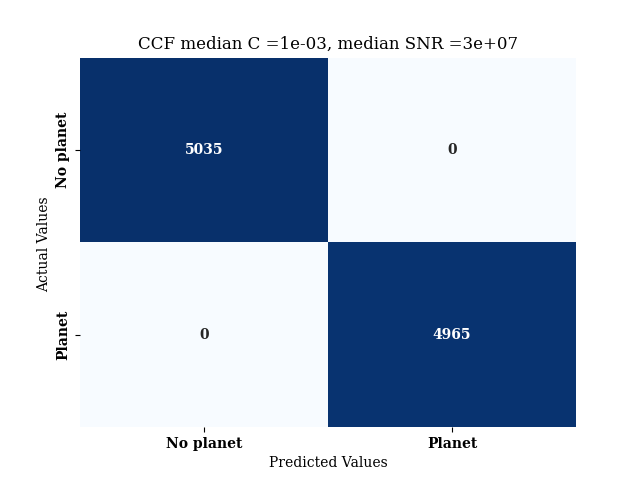
\includegraphics[scale =0.5]{images/Chapter3/confusion_ccf_1e-04_cmax_1e-02_dsnrmin_1e+07_dsnrmax_1e+08.png}
    \caption{Caption}
    \label{fig:ccf_cm}
\end{subfigure}
\hfill
\begin{subfigure}{0.4\textwidth}
    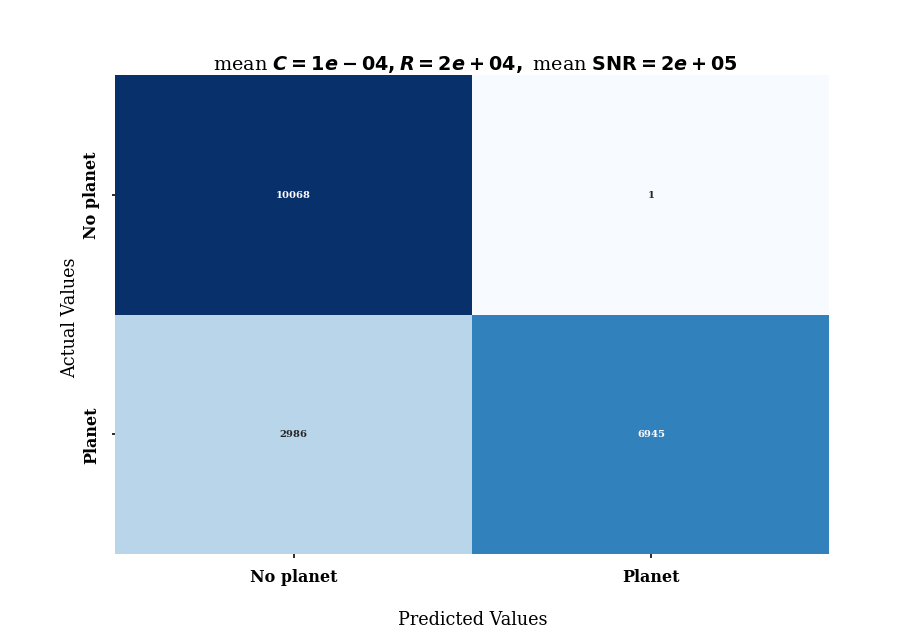
\includegraphics[scale=0.28]{images/Chapter3/ccf_cm_cmin_1e-5_cmax_1e-3_snrmin_1e5_snmax_1e6_R_20000.png}
    \caption{Caption}
    \label{fig:high contrast-ccf cm}
\end{subfigure}
\caption{CCF results}
\end{figure}
\Cref{fig:ccf_cm} shows a sample confusing matrix when generating a sample set with a median $C=10^{-3}$ with lowest $C=10^{-4}$ and the highest $C=10^{-2}$ and median $\rm{SNR}=10^{7}$.
In this case we have $\rm{FP}= 0$ and $\rm{TPR}=1.0$.
We also observe a case at higher contrast with mean $C=10^{-4}$ in \Cref{fig:high contrast-ccf cm} where we see that while with a $\rm{FP}=1$ we have a low number of false positives for $15000$ examples; we have a low $\rm{TPR}=0.67$ owing to both the higher contrast and the lower $\rm{SNR}$.
Note that for both figures, we are well beyond the detection limit based on \Cref{fig:detmat}.
However, this exercise is meant to illustrate the different ranges of training examples that are used with the ML algorithms.
Since higher $\rm{SNR}$ are more amenable to detection over a range of contrasts, they are the initial range of $\rm{SNR}$ that will be used for training.
\subsection{Low contrast results}
The low contrast performance was sequentially tested with random forests, MLP and autoencoders.
We will present the results here from the test set, the contrast ranges of $10^{-1}$ to $10^{-3}$ which is the "low contrast" region for the purpose of our analyses.
We present the results of the random forest for this contrast range for the validation data with $\approx 2500$ examples.
These training runs were conducted with two ranges $10^{-1}>C>10^{-2}$ which are presented in \Cref{fig:RF1e-1-1e-2} and for the range of $10^{-3}>C>10^{-2}$ in \Cref{fig:RF1e-3_1e-2}.
Similarly, for the autoencoder we split the results into the same contrast ranges and this is depicted in \Cref{fig:ae1e-2_1e-1} and $\Cref{fig:ae1e-3_1e-2}$

\begin{figure}[!ht]
\begin{subfigure}[!h]{0.4\textwidth}
    \centering
    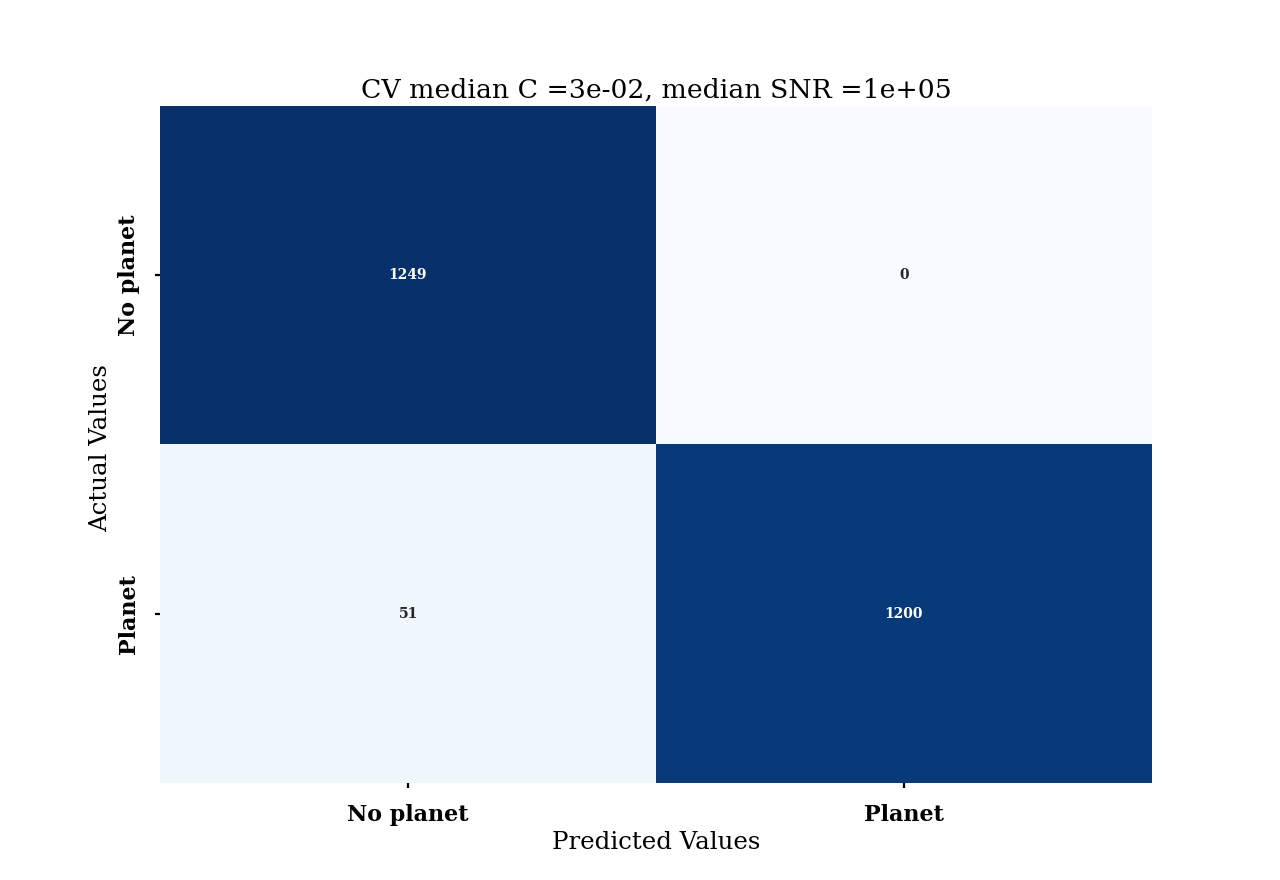
\includegraphics[scale=0.3]{images/Chapter3/confusion_RF_CV_1e-02_cmax_1e-01_dsnrmin_1e+04_dsnrmax_1e+06.png}
    \caption{Caption}
    \label{fig:RF1e-1-1e-2}
\end{subfigure}
\hfill
\begin{subfigure}{0.4\textwidth}
    \centering
    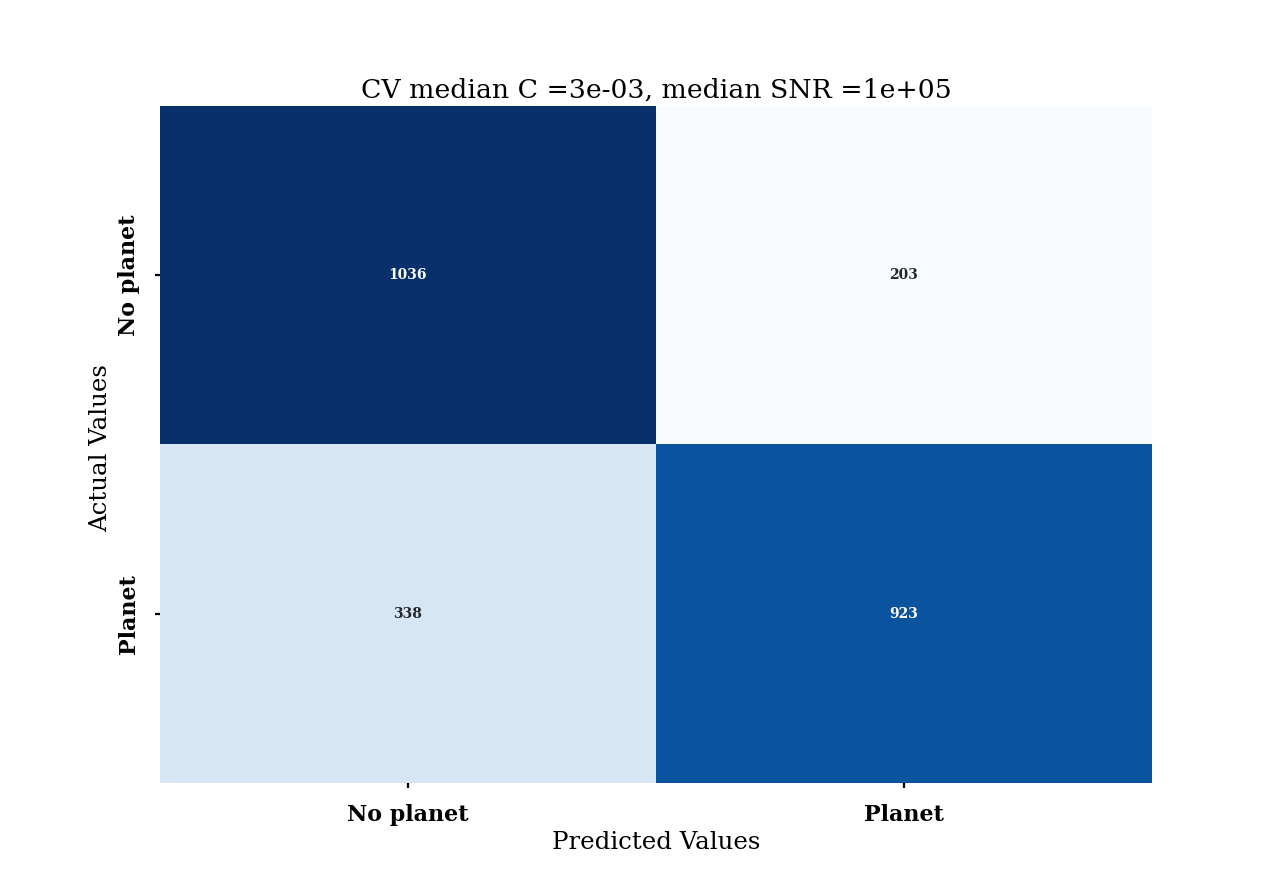
\includegraphics[scale=0.3]{images/Chapter3/confusion_RF_CV_1e-03_cmax_1e-02_dsnrmin_1e+04_dsnrmax_1e+06.png}
    \caption{Caption}
    \label{fig:RF1e-3_1e-2}
\end{subfigure}
\caption{RF results}
\end{figure}
\begin{figure}[!hb]
\begin{subfigure}{0.4\textwidth}
    \centering
    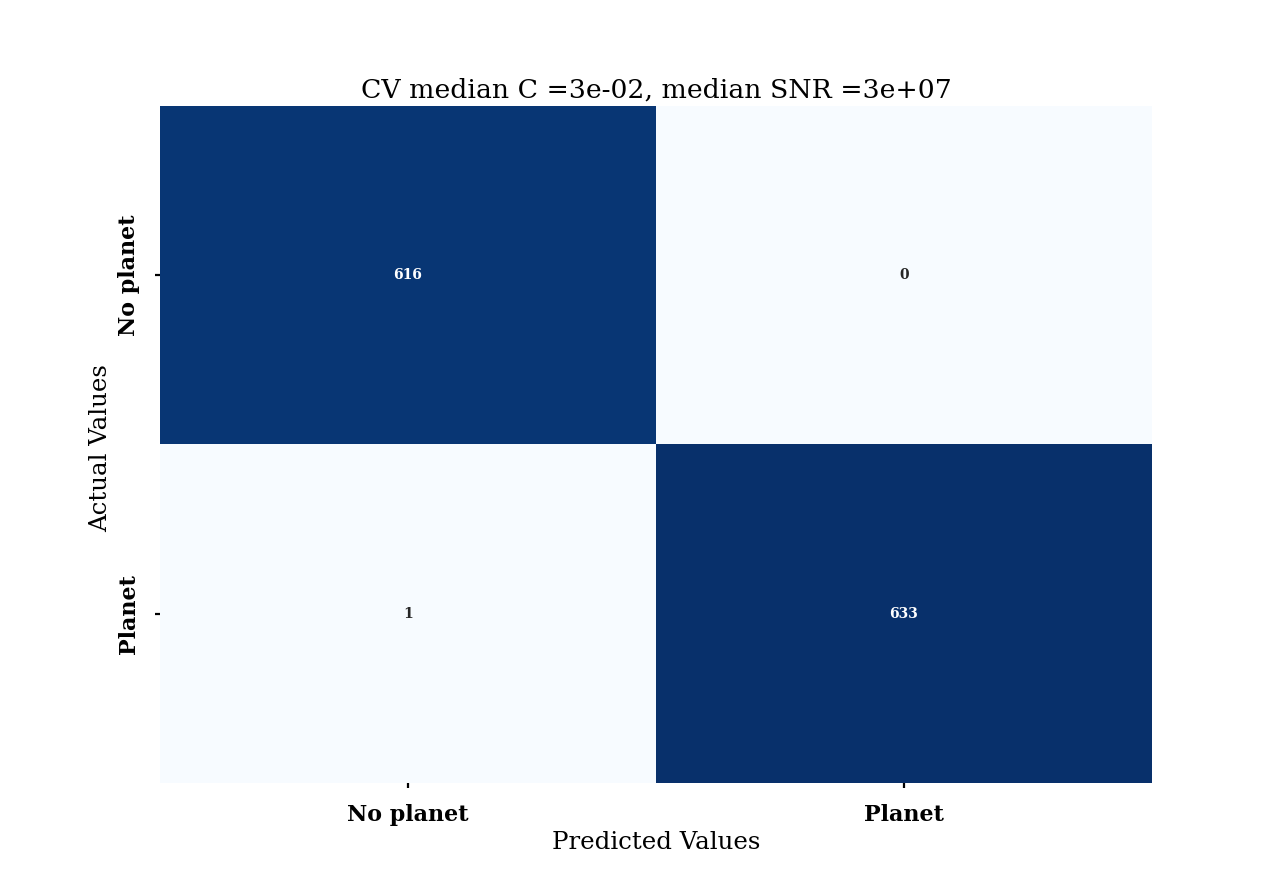
\includegraphics[scale=0.25]{images/Chapter3/confusion_transfer_sdae_CV_cmin_1e-02_cmax_1e-01_dsnrmin_1e+07_dsnrmax_1e+08.png}
    \caption{Caption}
    \label{fig:ae1e-2_1e-1}
\end{subfigure}
\hfill
\begin{subfigure}{0.4\textwidth}
    \centering
    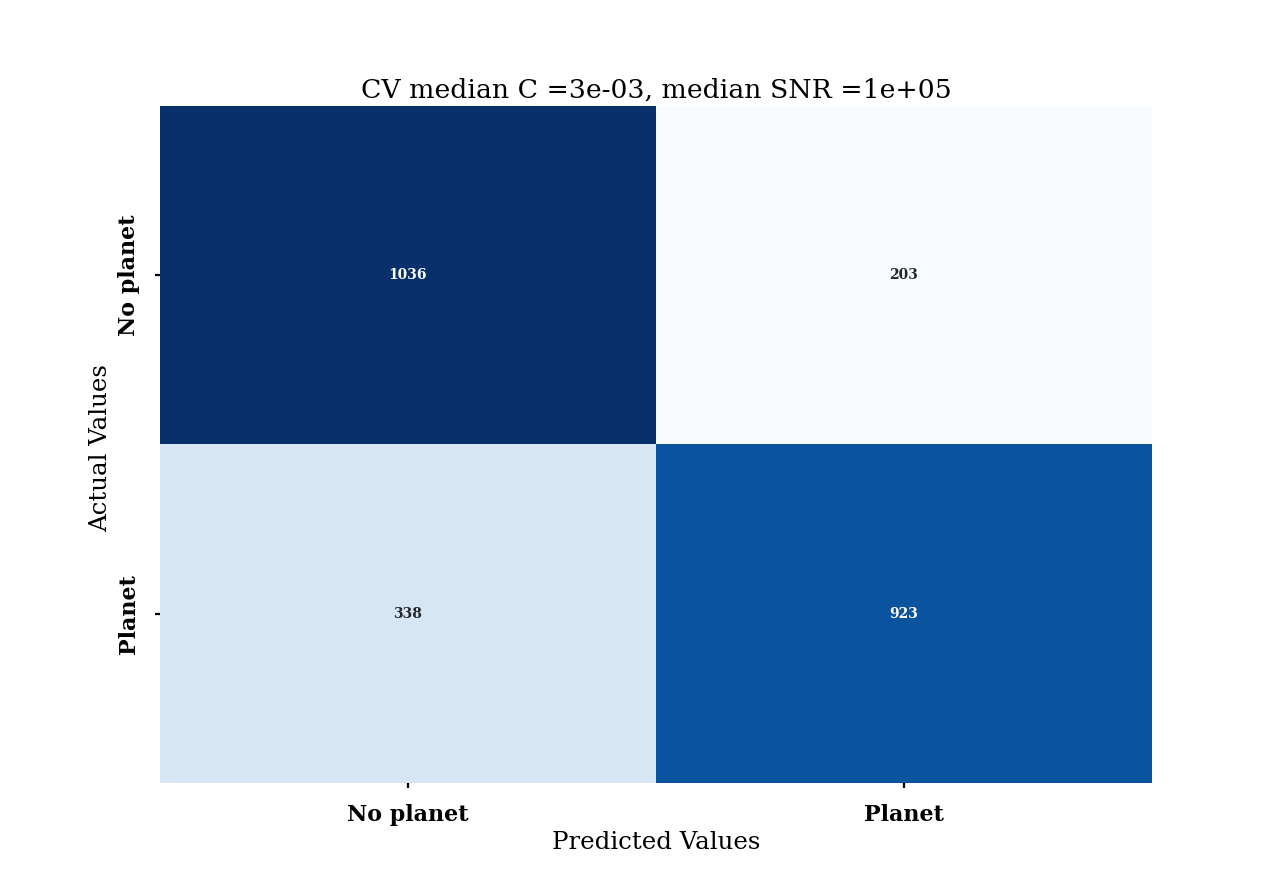
\includegraphics[scale=0.3]{images/Chapter3/confusion_RF_CV_1e-03_cmax_1e-02_dsnrmin_1e+04_dsnrmax_1e+06.png}
    \caption{Caption}
    \label{fig:ae1e-3_1e-2}
\end{subfigure}
\caption{AE results}
\end{figure}
When comparing the low contrast results its very interesting to look at \Cref{fig:ccf_cm} and \Cref{fig:RF1e-3_1e-2} and \Cref{fig:ae1e-3_1e-2} which are tested around the same contrasts.
The number of false positives is $0$ for the cross correlation and is $\approx 200$ for the ML aglorithms.
Note that this number is $\approx 10$ for a lower contrast on the left.
The $TPR\approx0.75$ for the ML algorithms but for the cross correlation based algorithm $\rm{TPR}=1$.
This is an interesting feature that when the contrast increases even in the low contrast cases the $\rm{TPR}$ plummets by a $\approx1/3$ and the number of false positives increases from $0$ to $200$.
Note that while the $\rm{TPR}$ remains high enough for the algorithm to be considered successful for mean $C\approx10^{-3}$, the number of false positives would deem the algorithm unsuitable for scientific usages.
At this stage, we can  say that ML algorithms have not achieved the necessary false positive requirement for scientific analysis.
However, in order to understand at what contrast the ML algorithms no longer learn new features we will also present the high contrast results.
\subsection{high contrast results}
We define a high contrast spectrum as that where $C<10^{-3}$.
We have already such a case of confusio matrix being produced for \Cref{fig:high contrast-ccf cm} where we see that $1$ false positive is identified for $10^{4}$ spectra  and the $\rm{TPR}\approx 0.7$.
We will now train and test this data with ML algorithms and these results are depicted in \Cref{fig:highcont_rf}
\begin{figure}
\begin{subfigure}{0.4\textwidth}
        \centering
        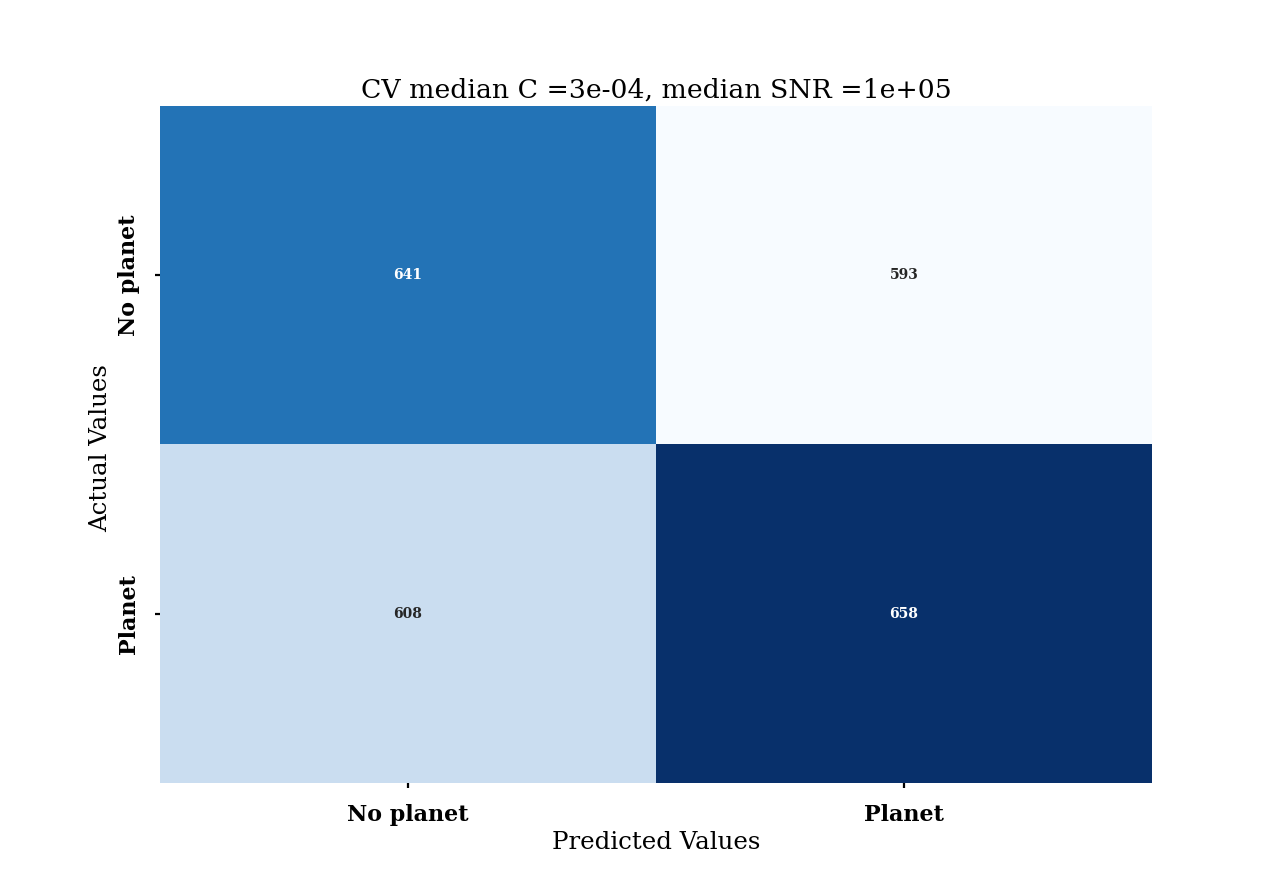
\includegraphics[scale=0.3]{images/Chapter3/confusion_RF_CV_1e-04_cmax_1e-03_dsnrmin_1e+04_dsnrmax_1e+06.png}
        \caption{Caption}
        \label{fig:highcont_rf}
\end{subfigure}
\hfill
\begin{subfigure}{0.4\textwidth}
        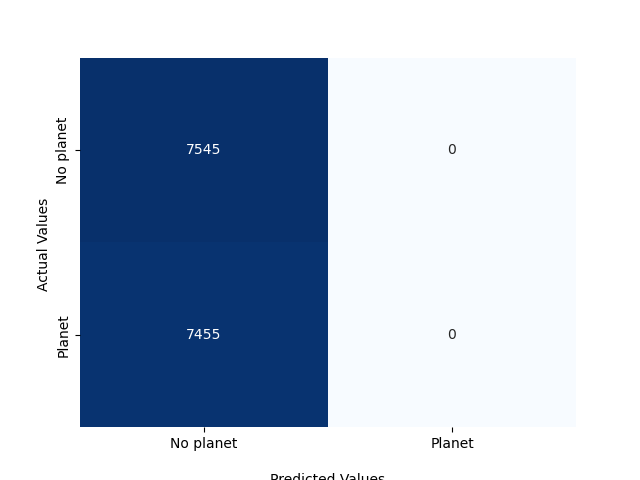
\includegraphics[scale=0.4]{images/Chapter3/confusion_mlp_1e-5_keras_train.png}
        \caption{Caption}
        \label{fig:highcont_mlp}
\end{subfigure}
\vfill
\begin{subfigure}{0.5\textwidth}
        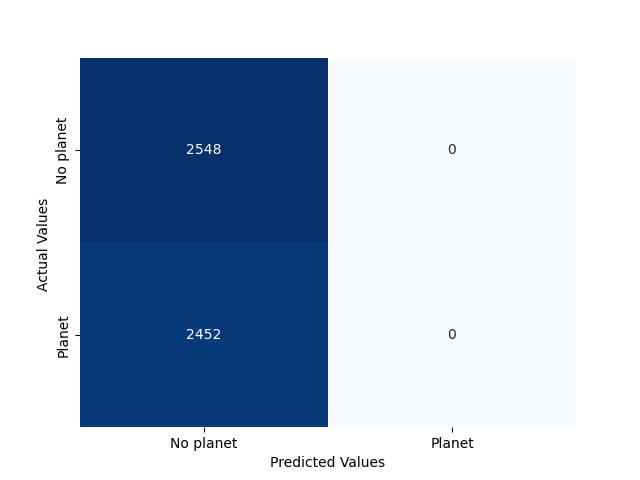
\includegraphics[scale=0.4]{images/Chapter3/confusion_ae_CV_lowcont_1e-5.png}
        \caption{Caption}
        \label{fig:highcont_ae}
\end{subfigure}
\label{figs:highcont}
\end{figure}
\textcolor{blue}{[TODO: 1. Training CM for both low and high contrast for all the algorithms
2. Make sure the CM are in the same SNR 
3. Have CM from two different ranges of SNR so its clear that its only contrast and not SNR which is the problem]}
\section{Discussion}
In this chapter, we have explored the use of three different ML algorithms in testing the detection hypothesis.
We were unable to progress beyond  testing the algorithms themselves to subsequently test the hypotheses themselves.
In this discussion section we will discuss what are the reasons for the poor results from ML algorithms.
\subsection{Random forest feature importances}
From the confusion matrices \Cref{fig:ae1e-2_1e-1} and \Cref{fig:RF1e-1-1e-2} it is clear that the training on very low contrasts where the planet is about $10$th as bright as the host star allows the ML algorithms to train effectively and produce the necessary confusion matrices as desired by our problem statement.
From these confusion matrices, it appears that as we increase the contrast the ability to classify drops off quite rapidly.
If this is indeed the case, what features does the ML algorithm learn in the lowest contrast that seem to disappear in the higher contrasts.
In order to answer this question we performed a very specific experiment by generating spectra for an exoplanet with exactly the same $\rm{T_{eff}}$ and $\rm{\log(g)}$ and train the random forest for different contrasts.
Note that even this case we get the exact same confusion matrices.
\begin{figure}
    \centering
    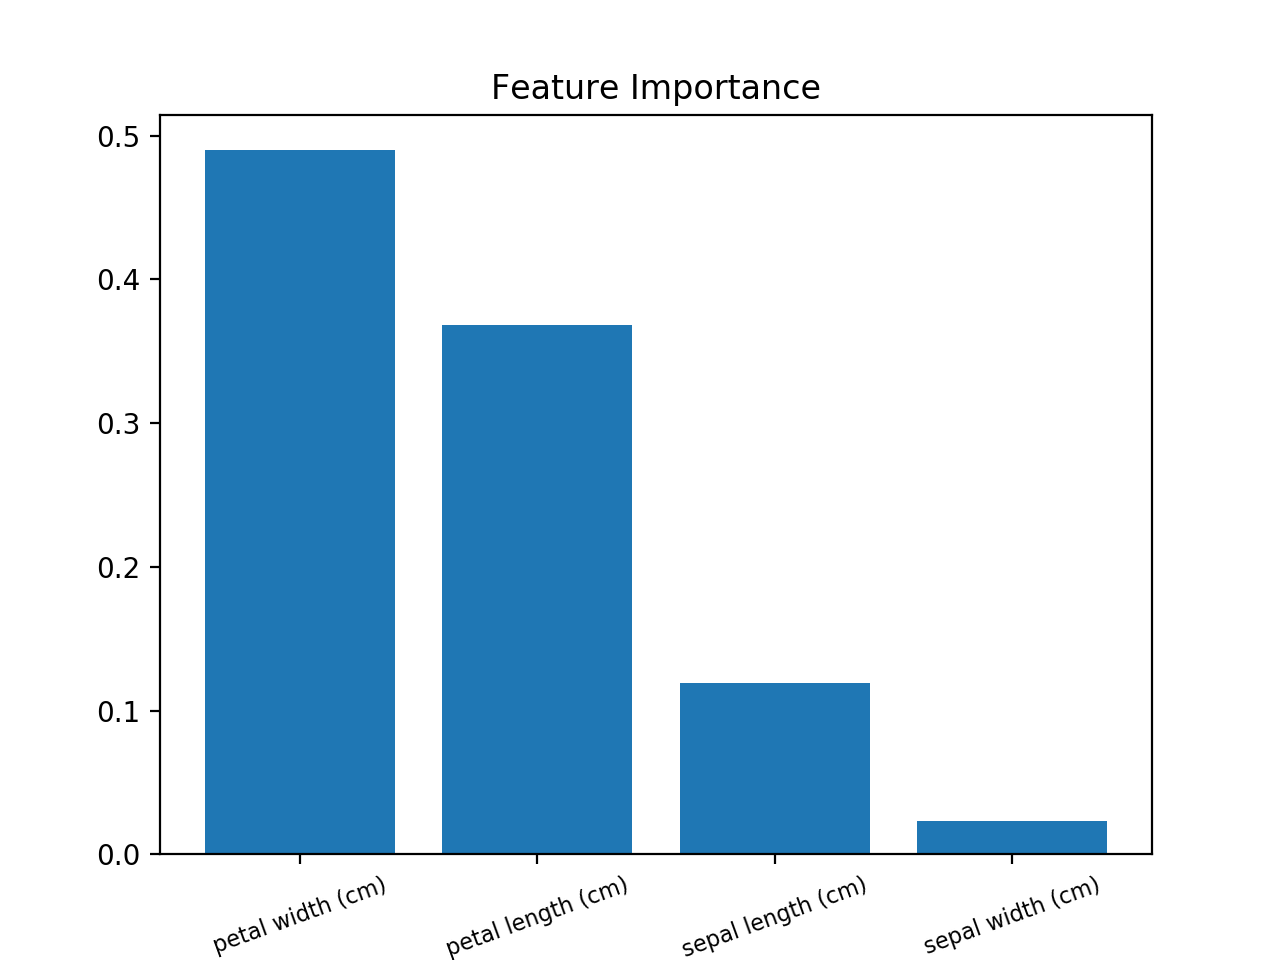
\includegraphics[scale=0.5]{images/Chapter3/feature_importances_Randomforest.png}
    \caption{Caption}
    \label{fig:RF-C-importances}
\end{figure}
Thus we produce \Cref{fig:RF-C-importances} using the same $\rm{SNR}$ and different values $C$.
The feature importances are plotted as function of $\lambda$ and should therefore track the importance of the wavelength bins.
In this figure, the uppermost dark panel indicates the template that was used to generate spectra to train with different contrasts.
The lower panels indicate the featrue importances produced by different random forest models.
The goal of our training is to generate feature importances that are a mirror image of the first panel in this image.
The first panel in this image represents the spectral features which are unique to an exoplanet that are not shared by either the noise or the stellar spectrum. 
This means that the features that the ML algorithms need to learn are the features uniquely present in the exoplanet spectrum. 
By training the ML algorithms with different types of spectra, we attempted to produce a plethora of features that would allow an ML algorithm to generalize. 
However, even when we restrict this problem to exactly one type of exoplanet we see that the features learnt with the changing contrasts are highly limited by the contrast.

One of the first noteworthy things about \Cref{fig:RF-C-importances} is the low values of the feature importances when compared to more `classical' feature importances such as \Cref{fig:RF sample FI}. 
While there is a relative gradient at the lowest contrast, the mean value is quite low.
This of course is a function of having a large number of absorption features which means that when no one feature is more important than the others we will have the importances distributed over many wavelengths. 
Our view on this plot is that while there does seem to be some amount of learning of the relative importances,the extremely low value of each importance actually seems to indicate that the model is unable to train robustly and learn all the features.
The second noteworthy point on this graph is the virtual disappearance of importances as the contrast increases and $C$ value decreases.
There seems to be some type of overfitting for the noise we can see a slight curving of the importances with the increasing wavelength.
When we look at the same feature importances for a low contrast and changing $\rm{SNR}$ we can see the same kind of behaviour in \Cref{fig: RF-SNR-featureimportances}.
We see that for the highest $\rm{SNR}$ the feature importances follow the same pattern as in \Cref{fig:RF-C-importances} and then for the same low contrast spectrum we see the feature importances disappearing as we decrease $\rm{SNR}$.
\begin{figure}
    \centering
    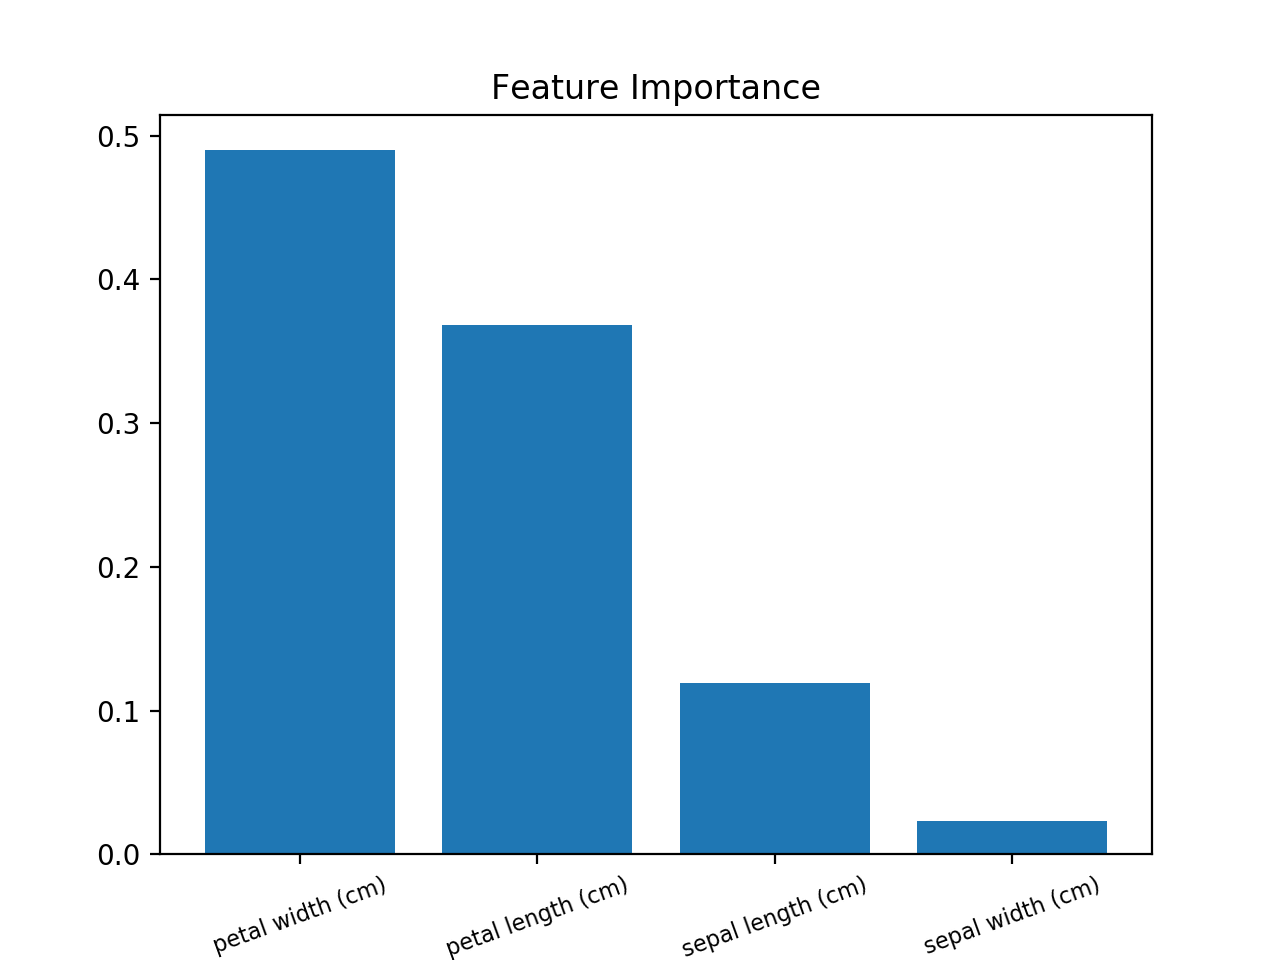
\includegraphics[scale=0.5]{images/Chapter3/feature_importances_Randomforest.png}
    \caption{\textcolor{blue}{Use the correct plot here}}
    \label{fig: RF-SNR-featureimportances}
\end{figure}
This behaviour attests to the most important inference of this part of my thesis,
In order for ML algorithms to be able to train and generalize on spectra from direct images the data needs to be both low contrast and high $\rm{SNR}$ as described in \Cref{chap:III.3}.
In the next subsection we will discuss why this form of problem statement is not very appropriate for ML algorithms.

\subsection{On the unsuitability of ML algorithms to test the detection and characterization hypotheses}
At the beginning of this part in \Cref{chap: III.1}, we stated that ML algorithms had the ability to process multiple datasets rapidly and with high precision. 
We also stated the ability of ML algorithms to draw inferences from diverse data sources.
In that sense we have developed our ML based algorithms to train on spectral data from multiple spectral channels.
We have identified the `best' quality data by defining a $\rm{SNR}$ which is a pure signal metric to define a spectrum.
We have also used $C$ as a parameter to inject astrophysics into the problem.
But these have served only as scaffolding to the fundamental question, which is whether given diverse spectral features in a high quality astrophysical spectrum can an ML algorithm train and generalize to detect exoplanets and further to characterize them.
To this effect we trained an ensemble algorithm and two deep learning algorithms.
We found that the best spectra to train were indeed the ones with lowest contrast and highest $\rm{SNR}$.
We also learnt that the features that for example a random forest based algorithm learns is a mild version of the spectral features shows that ML algorithms are indeed capable of learning some features.
However, what is also clear is that ML algorithms are not able to diversify these features to pick up higher contrast or lower $\rm{SNR}$ exoplanets in spectra.

To verify that the features are not transferrable, we saved the weights of the deep learning algorithms and used them as the starting weights to train higher contrast companions. 
We found that the confusion matrices are exactly the same. 
When we tried to use the same weights tuned to detect lower contrast exoplanets we found that the neural network never detects the exoplanet. 
This means that the features learnt on low contrast or high $\rm{SNR}$ are not general enough to be used to detect exoplanets.
This is the fundamental reason why we cannot compose a detection matrix using ML algorithms.
Consequently, we cannot test the detection hypothesis using ML algorithms.

The characterization hypothesis, relies on the ability of an algorithm to primarily detect the spectrum. 
We saw with the cross correlation based algorithm that when an exoplanet is detectable in the spectrum, it can be characterized with a consistent error bar which in turn can be reduced by perfectly dividing out the stellar contamination.
However, ML algorithms have proven to be incompetent in learning features to even test the detection hypothesis and therefore it does not behove to test the characterization hypothesis which relies on the very same features.
Note that this thesis has stopped short of composing the characterization matrix for those exoplanet spectra that can be detected due to the lack of time.
\chapter{Discussion and conclusion}
This part of the thesis has had two broad goals for using direct imaging spectra,
\begin{enumerate}
    \item to define whether detectability and characterization of exoplanets using spectra was possible and if so what is the biggest factor in this detectability and characterization,
    \item and can the use of modern ML algorithms improve this detectability and characterization, and if so can this be quantified using a common metric that could be shared by both ML and non ML algorithms.
\end{enumerate}
We have tested these ideas in different ways and in this chapter we will discuss the different aspects of testing both these ideas.
To start we will discuss how the detection and characterization hypotheses are relevant to achieving goal 1 above.
In this context we will discuss the relevance of the detection and characterization matrix and how they aid us in exploring idea 1.
Then we will discuss how the use of ML algorithms has been ineffective in exploring the scientific idea 1 and how this means that they are unsuitable to use to explore idea 2.
Finally, we will discuss the broad reasons around ML algorithms not being very successful and what are the steps that can be taken to mitigate this issue.
\section{The detection and characterization hypotheses}
The broad goal of this part of my thesis was to evaluate whether spectra could be use to detect exoplanets and to characterize them by using the same spectral features.
This implies that the absorption features that are typical to an exoplanet will be well discriminated from those of the host star and if the spectrum is of sufficient quality with enough of these absorption lines.
The relevant question, therefore, is when the stellar and planetary spectra are combined would a well tuned algorithm be able to detect the exoplanetary features well enough to not ony be able to discover an exoplanet but predict with a known level of uncertainty the kind of planet it is.

Based on these questions, we defined the detection and characterization hypotheses, to study the limits of detection of a warm Jupiter and its corresponding characterization.
These hypotheses allowed us to define the problem statement that we are aiming to test and justify the reason to reject some results and accept others. 
The hypotheses also validate the benchmark by which we will evaluate algorithms to test these hypotheses.
For instance, the detection hypothesis states that so long as there are exoplanet absorption features in a spectrum, the exoplanet is detectable in sufficiently high quality spectrum. 
We establish that the quality of a spectrum would be defined by the number of photons it gathers, and if they are sufficiently high we would be able to detect an exoplanet. 
This, however, does not sufficiently define the sensitivity of an algorithm to detect exoplanets. 
Therefore to define how sensitive an algorithm is we defined the contrast $C$ at which an exoplanet is present with respect to the host star.
We then developed a detection matrix to define this sensitivity and test the detection hypothesis.
The detection matrix allows us to define if at the lowest contrast (highest value of $C$) it is still possible to detect the exoplanet for all the different quality spectra.
In principle, the contrast at which a detection is claimed is a measure of how an algorithm interprets spectra and not a test of the hypothesis.
The hypothesis is tested by checking if an exoplanet can be detected for different quality of spectra. 
We tested this hypothesis extensively by considering spectra of very low $\rm{SNR}$ and running it through our cross correlation based detection algorithm.
We found that the detection matrix tests the detection hypothesis for even very low values of $\rm{SNR}$ and for the highest $\rm{SNR}$ we found that the exoplanet was detected at the highest contrasts $C=10^{-6}$.
For the detection hypothesis, this means that it was tested and verified at a $\rm{SNR}\ge10^{5}$.
For lower $\rm{SNR}$s we are limited by the sensitivity of the algorithm. 
This is one of the major contributions of this part of the thesis that we have produced a detection matrix to test the detection hypothesis which also serves to validate the sensitivity of an algorithm.

The characterization hypothesis defines that the characteristic parameters of the exoplanet, namely $\rm{T_{eff}}$ and $\log(\rm{g})$ can be estimated through its spectra with well quantified error bars.
We defined a characterization matrix that allows us to infer the mean values of these characteristic parameters and estimate their uncertainty.
When we run the spectra through our cross correlation based algorithm, we found two salient results,
\begin{enumerate}
    \item we found that the characterization error bar became consistent at $\rm{SNR_{ccf}}\ge3$ and that this value does not change with increase in $\rm{SNR}$ but,
    \item this uncertainty changed for lower contrasts and in fact this uncertainty became the lowest for $C=1$ i.e a case of where stellar signal was perfectly removed from the spectrum.
\end{enumerate}
These two results fundamentally validate the ideas that,
\begin{enumerate}
    \item the characteristic parameters of the exoplanet in the spectrum can be estimated with a known accuracy when the exoplanet is detectable and
    \item this characterization is impacted by the amount of residual stellar features that are present in the spectrum.
\end{enumerate}
Both of these derivations are corollaries to the characterization hypothesis which states that \textit{when} the exoplanet is present in the spectrum we are able to characterize the spectra with constant error bars.
This thesis thus defines this word \textit{when} to be $\rm{SNR_{ccf}}\ge3$.
The second idea that stellar contamination is the fundamental reason for error in the characterization of the exoplanet allows us to appreciate the limitation of characterization algorithms when the characteristic is a broad parameter such as $\rm{T_{eff}}$.

Thus, the detection and characterization hypotheses have been well tested and verified with the cross correlation algorithm. 
This allowed us to rule out the fundamental question of whether this problem is well defined. 
Secondly it also now allowed us to set a benchmark and parameter space for follow up algorithms.
The fact that the sensitivity of the cross correlation based detection algorithm was the highest at $\rm{SNR}>10^{5}$ pointed to that value being the cut off for the best quality spectra.
It also allowed us to state that scientifically it provides reasonable basis to verify that algorithms satisfy the detection hypothesis at these values of $\rm{SNR}$ before we undertake a study of their sensitivity  to detection at lower $\rm{SNR}$.
Finally, the tests of the characterization hypothesis allowed us to link the detection and characterization at $\rm{SNR_{ccf}}>3$.
Note that this still cannot be called a detection but this allows us to make a scientific justification to produce a characterization matrix before testing the detectability of an exoplanet rigorously.
\section{Why did the ML algorithms fail where the cross correlation based algorithm succeeded?}
The detection and characterization matrices allow us to test the detection and characterization hypotheses respectively.
The goal for ML algorithms was to operate on the same data and the same evaluation criterion to ensure we are able to compare both the types of algorithms.
We chose to start training and testing ML algorithms with the highest $\rm{SNR}$ spectra, with the goal as first establish the sensitivity of ML algorithms on the best quality spectra.
This would have allowed us to establish the detection sensitivity of an ML based algorithm at a $\rm{SNR}$ where the detection hypothesis was satisfied by the cross correlation based for the highest contrast.

As a start we had planned to test the ability of ML algorithms to detect spectra with exoplanet features in them consistently at a specific value of $R,\rm{SNR}$ for different values of $C$ starting from $10^{-1}$ down to $C=10^{-6}$.
We aimed to evaluate the detection sensitivity of these algorithms using confusion matrices.
As has been clear from the results, the highest contrast that ML algorithms can detect exoplanets is $10^{-3}$.
An analysis of the results showed that the data features that the ML algorithms need to learn to detect exoplanets disappear beyond this contrast.
Naturally, producing a detection matrix is moot at this point because ML algorithms do not seem to be able to test the detection hypothesis. 
Evidence, also shows that if you are unable to detect the exoplanet it is not possible to test the characterization hypothesis.
Consequently, this thesis concludes that ML algorithms are not appropriate to test these hypotheses in this manner.
The question therefore is why these ML algorithms failed where a cross correlation based algorithm had succeeded.
There are several reasons this could be true we list a few of them below,
\paragraph{1. the lack of significant differentiating features in spectra for ML algorithms to learn from:\\}
One of the major requirements for ML algorithms to separate the $y=0$ and $y=1$ cases would be the presence of clear differentiating features between the two classes.
When we look for example at \Cref{fig:compare-specsnr=5.24} and \Cref{fig:compare-specsnr=3000} it is fairly evident that \Cref{fig:compare-specsnr=3000} contains several spectral bins that contain differentiating features, which may not be so evident in \Cref{fig:compare-specsnr=5.24}.
This is reflected in confusion matrices produced by the ML algorithms on the same parameter spaces.
We clearly observe that the matrices produced with the low contrast exoplanets has very good $\rm{TPR}$ and low false positives.
But as the contrast increases, we notice the confusion matrices producing more false negatives and in the case of random forests more false positives as well.
All these indicate that while in the lower contrast cases the algorithms have features that are different between $y=0$ and $y=1$, as the contrast increases these features get washed away by stellar signal.
This is why even at the higher $\rm{SNR}$ contrast seems to play such an important role.
Thus, we also see that as the contrast increases, deep learning algorithms see only $y=0$ cases whereas random forests get confused more with the noise.

\paragraph{2. the presence of large number of wavelength bins that do not contain discriminating information:\\}
the large number of wavelength bins are supposed to act as features to ML algorithms which allows them to learn the difference between the $y=0$ and $y=1$ cases, provided there are enough wavelength bins with features.
The cross correlation based algorithm uses this measure to produce a strong cross correlation signature by accounting for the small amounts of information in each wavelength bin. 
This has caused problems for many detection problems in the past where false correlations due to atmospheric lines, particularly the Telluric absorption.
The assumption at the beginning of this part was that there was enough information in each wavelength bin which allows the cross correlation to detect the exoplanets and therefore should be sufficient for ML algorithms as well.
However, this appears to have been an incorrect assumption, because if this was true then either increasing the contrast or increasing the $\rm{SNR}$ should have had lesser effect than it currently has.
If the ML algorithms were purely influenced by the astrophysical features, then we would notice an ML algorithm continuing to detect exoplanets at low $\rm{SNR}$ or at the very least be less sensitive to changing $\rm{SNR}$ and a reverse effect would be noticed if the ML algorithms were only affected by the signal in the data. 
But we notice that both the $\rm{SNR}$ needs to be high and the $C$ has to be low for ML algorithms to detect exoplanets.
This is a sign that that not only are there no differentiating features at higher contrasts and lower $\rm{SNR}$ but that intrisically the large number of wavelength bins don't contain enough information. 
A counter point to this is that it is possible that ML algorithms would be trained if we limit the spectra to certain wavelength bins rather than the whole spectrum.
\paragraph{3. finally the presence of photon noise which leads to a lot of variance in features:\\}
astronomical observations have at the very least photon noise. 
This is very basic and intrinsic noise that is always present in astronomical data.
This noise produces intrinsic randomness in the data and also washes out crucial features in the data. 
We see that both the cross correlation and ML based algorithms are both impacted by this.
While the sensitivity of the cross correlation algorithm is limited by this noise, for the ML algorithms it appears to hamper both training and validation of the data.
This noise seems to also produce a large amount of confusion in random forests.
When the noise levels are decreased at a constant contrast $C>10^{-3}$ there seems to be minimal impact of noise on the algorithms. 
We see this as an effect of the nature of photon noise. 


\section{Conclusions and limitations of the study}
This study has had several interesting results and contributions to the field of exoplanet detection and characterization.
We will first list the notable contributions and then discuss the many limitations of this study.

\subsection{Conclusions of this study}
The conclusions in this study follow three major axis points, the scientific hypotheses developed for this study, followed by the algorithms and finally generalised conclusions of the study.
\paragraph{The detection and characterization hypotheses\\}
In the field of direct exoplanet detection, the use of spectra are well known and somewhat well explored.
This part of the thesis primarily explored the idea of whether it was possible to simultaneously detect and characterize exoplanets using their spectra alone.
In this part we have defined the detection hypothesis which was tested using the detection matrix and the characterization hypothesis which was tested using the characterization matrix.
We defined both these hypotheses and their evaluation metrics to be compatible with both ML and non-ML algorithms. 
We then generated data that could be used for both types of algorithms and which have a basis in astrophysics.

\paragraph{A cross correlation based detection and characterization algorithm:\\}
We developed an algorithm that cross correlates template spectra with target data spectra, and we interpret these results to compute the detection and characterization matrices.
We discovered that the sensitivity of detection of an exoplanet is limited by the $\rm{SNR}$ of the spectrum. 
We also found that the detection hypothesis is satisified for all values of contrast at the highest $\rm{SNR}$.
The characterization of an exoplanet is limited by the same parameters as the detection, but at a lower threshold of the detection parameter we obtain a stable uncertainty but a value higher than what is demanded by the scientific community.
We found that the perfect characterization of an exoplanet is limited by the stellar contamination and when stellar contamination is perfectly removed then we have perfect characterization with stable uncertainties.

\paragraph{generalized conclusions:\\}
This study has attempted to understand the interaction between detectability, characterization and the improvement that ML algorithms bring to this interaction.
We have concluded that exoplanet detection using cross correlation algorithms is the ultimate test of the presence of an exoplanet and characterization serves as a clue to the presence of the presence of this exoplanet given very specific conditions (for ex: $\rm{SNR_{ccf}}>3$).
This study has also learnt that ML algorithms, no matter how advanced, are severely impacted by both noise and the contrast of the exoplanet.
The changing $\rm{SNR}$ impacts the cross correlation by reducing its sensitivity but in case of the ML based algorithms we notice that both changing $\rm{SNR}$ and $C$ impacts the detection sensitivity.
\subsection{Limitations of this study}
This study has certain specific limitations fundamentally related to its scope, the data used and extent of exploration of the use of ML algorithms.
\paragraph{an unfair comparison between the cross correlation based and ML based algorithms:\\}
while comparing the performance of the cross correlation based algorithms with those of the ML based algorithms it appears that this kind of problem statement is better suited for a cross correlation kind of algorithm which only evaluates the similarity between spectra.
Since we generate large number of spectra which are subject to only random modifications, this problem  could be better suited to an unsupervised approach than a supervised one 
\paragraph{lack of realistic variation in the data:\\}
so ML doesn't train
\paragraph{the choice of ML algorithms:\\}
maybe a more interesting choice than a safe one could have helped
\paragraph{non use of specific molecules:\\}
Use of molecules is well established but we chose not to.

\section{Next steps and how this can feature sparsity be countered.}
One of the major reasons to not be able to compose a detection matrix with ML algorithms has been the sparsity of features in the spectra.
As we saw with \Cref{fig: RF-SNR-featureimportances}, it was clear that no matter the contrast or the $\rm{SNR}$ the feature importances never were strong enough to reproduce spectral features.
While at lower contrasts we could still some features, these would have disappeared in a more realistic and varying dataset.
This makes it unambiguous that the data needs sufficient feature to be able to detect exoplanets.

It is also clear from our analysis that basic characterization of an exoplanet using its spectrum is fundamentally related to its detection. 
Therefore, it is imperative to study the best way to present ML algorithms data to detect exoplanets at high contrasts.
We have also seen that $\rm{SNR}$ provides a loosely but not wholly reliable metric to evaluate if the data is sufficiently diverse to train a ML algorithm or contains sufficient features.
Therefore, we need to find a metric that gives us insight into the data that is presented to ML algorithms for training.
In the part that follows this, we will study how ML algorithms behave when provided with a feature rich dataset and when compared using a metric that sees the same features as the ML algorithm.

